% Build with latexmk; watch with latexmk -pvc. See assets/README.md.
\documentclass[notes=show]{beamer}
%%%%%%%%%%%%%%%%%%%%%%%%%%%%%%%%%%%%%%%%%%%%%%%%%%%%%%%%%%%%%%%%%%%%%%%%%%%%%%%%%%%%%%%%%%%%%%%%%%%%%%%%%%%%%%%%%%%%%%%%%%%%%%%%%%%%%%%%%%%%%%%%%%%%%%%%%%%%%%%%%%%%%%%%%%%%%%%%%%%%%%%%%%%%%%%%%%%%%%%%%%%%%%%%%%%%%%%%%%%%%%%%%%%%%%%%%%%%%%%%%%%%%%%%%%%%
\AtBeginSubsection[
  {\frame<beamer>{\frametitle{Outline}   
    \tableofcontents[currentsection,currentsubsection]}}%
]%
{
  \frame<beamer>{ 
    \frametitle{Outline}   
    \tableofcontents[currentsection,currentsubsection]}
}
\usepackage{ulem}
\usepackage{pdflscape}
\setbeamertemplate{caption}{\insertcaption}
\usepackage{color,xcolor,ucs}
\usepackage{beamerthemesplit}
\usepackage{graphicx}
\usepackage{amsmath}
\usepackage{adjustbox}
\usepackage{pdfpages} 
\definecolor{mintgreen}{rgb}{0.6, 1.0, 0.6}
\makeatletter
\@addtoreset{subfigure}{framenumber}% subfigure counter resets every frame
\makeatother
\newcommand*{\Scale}[2][4]{\scalebox{#1}{$#2$}}%
\newcommand*{\Resize}[2]{\resizebox{#1}{!}{$#2$}}%
\usepackage{amsfonts}
\usepackage{booktabs}
\usepackage{color,soul}
\usepackage{pdfpages}
\setboolean{@twoside}{false}
\usepackage{amsmath}
\usepackage{pdflscape} 
\usepackage{eurosym}
\usepackage{amstext} % for \text
\DeclareRobustCommand{\officialeuro}{%
  \ifmmode\expandafter\text\fi
  {\fontencoding{U}\fontfamily{eurosym}\selectfont e}}
% Compatibility with the caption package shipped in TeX Live 2018.
\makeatletter
\providecommand\@@magyar@captionfix{}
\makeatother
\usepackage[caption = false]{subfig}
\usepackage{appendixnumberbeamer} 
\usepackage{graphicx}
\usepackage{mathpazo}
\usepackage{hyperref}
\usepackage{multimedia}
\usepackage{graphicx}
\usepackage{multirow}
\usepackage{subfig}
\usepackage{verbatim}
\usepackage{booktabs, multicol, multirow}
\setcounter{MaxMatrixCols}{10}
\input{assets/Macros.tex}
\AtBeginSection[]
{
  \begin{frame}[noframenumbering]
    \frametitle{Outline for section \thesection}
    \tableofcontents[currentsection]
  \end{frame}
}


\usepackage{xcolor,soul}
\renewcommand<>{\hl}[1]{\only#2{\beameroriginal{\hl}}{#1}}

% https://tex.stackexchange.com/questions/41683/why-is-it-that-coloring-in-soul-in-beamer-is-not-visible
\makeatletter
\newcommand\SoulColor{%
  \let\set@color\beamerorig@set@color
  \let\reset@color\beamerorig@reset@color}
\makeatother
\SoulColor
\AtBeginSection{\frame{\sectionpage}}

\newsavebox\mybox
\newenvironment{aquote}[1]
  {\savebox\mybox{#1}\begin{quote}\openautoquote\hspace*{-.7ex}}
  {\unskip\closeautoquote\vspace*{1mm}\signed{\usebox\mybox}\end{quote}}

\newtheorem{proposition}[theorem]{Proposition}
\newtheorem{Assumption}[theorem]{Assumption}
\newenvironment{stepenumerate}{\begin{enumerate}[<+->]}{\end{enumerate}}
\newenvironment{stepitemize}{\begin{itemize}[<+->]}{\end{itemize} }
\newenvironment{stepenumeratewithalert}{\begin{enumerate}[<+-| alert@+>]}{\end{enumerate}}
\newenvironment{stepitemizewithalert}{\begin{itemize}[<+-| alert@+>]}{\end{itemize} }
\usetheme{Madrid}
\makeatletter
\setbeamertemplate{footline}
{
  \leavevmode%
  \hbox{%
  \begin{beamercolorbox}[wd=.333333\paperwidth,ht=2.25ex,dp=1ex,center]{author in head/foot}%
    \usebeamerfont{author in head/foot}\insertshortauthor~~\beamer@ifempty{\insertshortinstitute}{}{(\insertshortinstitute)}
  \end{beamercolorbox}%
  \begin{beamercolorbox}[wd=.333333\paperwidth,ht=2.25ex,dp=1ex,center]{title in head/foot}%
    \usebeamerfont{title in head/foot}\insertshorttitle
  \end{beamercolorbox}%
  \begin{beamercolorbox}[wd=.333333\paperwidth,ht=2.25ex,dp=1ex,right]{date in head/foot}%
    \usebeamerfont{date in head/foot}\insertshortdate{}\hspace*{2em}
%    \insertframenumber{} / \inserttotalframenumber\hspace*{2ex} % DELETED
  \end{beamercolorbox}}%
  \vskip0pt%
}
\makeatother
\usepackage{pdfpages}
\begin{document}
	\title[]{\large Instrumental Variables
	\vspace{0.5cm}
	}
	\author[Norris \& Saggio - Econ 628]{Sam Norris and Raffaele Saggio}
	\institute[]{UBC}
	\date{\today \\
}
	\maketitle

\section{Part I: Instrumental Variables}






\begin{frame}{Introduction}

\begin{itemize}
\item This lecture covers \textbf{instrumental variables} (IV) methods{\small{}\medskip{}
}{\small\par}
\item IV has been at the center of applied microeconometric research for
the last few decades{\small{}\medskip{}
}{\small\par}
\item IV methods pioneered by economists have been widely adopted in other
areas of empirical research{\small{}\medskip{}
}{\small\par}
\item We will begin by studying IV methods in a constant effects framework,
then circle back to reinterpret these methods in a world of heterogeneous
effects
\end{itemize}
\end{frame}

\begin{frame}{IV History}

\begin{itemize}
\item {\small{}Instrumental variables methods were developed to deal with
two seemingly unrelated problems\medskip{}
}{\small\par}
\item {\small{}Philip and Sewall Wright, 1920s: \medskip{}
}

\begin{itemize}
\item {\small{}Sought to estimate supply and demand relationships with data
on equilibrium prices/quantities\medskip{}
}{\small\par}
\item {\small{}This line of inquiry developed into the study of simultaneous
equations models (SEMs)\medskip{}
}{\small\par}
\end{itemize}
\item {\small{}Wald, 1940: Sought to estimate a regression line when the
regressor is measured with error\medskip{}
}{\small\par}
\item {\small{}Today IV is most often used as a method to eliminate omitted
variables bias in single-equation causal models}{\small\par}
\end{itemize}
\end{frame}
\begin{frame}
\frametitle{Outline}
\begin{enumerate}
\item Part 1: Constant Treatment Effect
\begin{itemize}
\item Simple IV: 1 instrument, 1 endogenous variable
\item Multiple Instruments: 2SLS 
\item IV as GMM
\item Overidentification Tests
\item 2SLS Mistakes
\item Pop-Quiz!
\item Many/Weak Instruments
\end{itemize}
\bigskip
\item Part 2: Heterogeneous Treatment Effects
\begin{itemize}
\item LATE Theorem
\item Compliers Characteristics 
\item Over-id tests with HTE
\end{itemize}
\end{enumerate}
\bigskip
Main reference: Mostly Harmless Econometrics. 
\end{frame}

\section{Constant Effects}
\subsection{Simple IV}
\begin{frame}{A Simple Causal Model}

\begin{itemize}
\item {\small{}Consider a simple constant-effects causal model:}{\small\par}
\end{itemize}
\begin{center}
{\small{}$Y_{i}(s)=\alpha+\rho s+\varepsilon_{i}$}{\small\par}
\par\end{center}
\begin{itemize}
\item {\small{}$Y_{i}(s)$ is $i$'s potential wage if s/he attends school
for $s$ years\medskip{}
}{\small\par}
\item {\small{}This additively separable function form implies constant
causal effects: $Y_{i}(s)-Y_{i}(s-1)=\rho\ \forall(i,s)$\medskip{}
}{\small\par}
\item {\small{}We observe schooling $S_{i}$ and earnings $Y_{i}(S_{i})$}{\small\par}
\end{itemize}
\end{frame}
\begin{frame}{A Simple Causal Model}

\begin{itemize}
\item {\small{}Equation for observed earnings:}{\small\par}
\end{itemize}
\begin{center}
{\small{}$Y_{i}=\alpha+\rho S_{i}+\varepsilon_{i}$}{\small\par}
\par\end{center}
\begin{itemize}
\item {\small{}This is a structural equation, not a regression, so no guarantee
that $Cov(S_{i},\varepsilon_{i})=0$\medskip{}
}{\small\par}
\item {\small{}Project $\varepsilon_{i}$ on to unobserved ability $A_{i}$:}{\small\par}
\end{itemize}
\begin{center}
{\small{}$\varepsilon_{i}=\gamma A_{i}+v_{i}$}{\small\par}
\par\end{center}
\begin{itemize}
\item {\small{}$Cov(A_{i},v_{i})=0$ by definition; assume $Cov(S_{i},v_{i})=0$\medskip{}
}{\small\par}
\item {\small{}Unobserved ability $A_{i}$ is a potential source of omitted
variable bias}{\small\par}
\end{itemize}
\end{frame}


\begin{frame}{Long and Short Regressions}

\begin{itemize}
\item {\small{}``Long'' regression:}{\small\par}
\end{itemize}
\begin{center}
{\small{}$Y_{i}=\alpha+\rho S_{i}+\gamma A_{i}+v_{i}$}{\small\par}
\par\end{center}
\begin{itemize}
\item {\small{}``Short'' regression:}{\small\par}
\end{itemize}
\begin{center}
{\small{}$Y_{i}=\alpha_{s}+\rho_{s}S_{i}+v_{is}$}{\small\par}
\par\end{center}
\begin{itemize}
\item {\small{}OVB formula:}{\small\par}
\end{itemize}
\begin{center}
{\small{}$\rho_{s}=\rho+\gamma\dfrac{Cov(S_{i},A_{i})}{Var(S_{i})}$}{\small\par}
\par\end{center}
\begin{itemize}
\item {\small{}The regression we've got (short) is not the regression we
want (long)\medskip{}
}{\small\par}
\item {\small{}IV is a method for obtaining the long regression coefficient
without data on the omitted regressor $A_{i}$}{\small\par}
\end{itemize}
\end{frame}

\begin{frame}{Instrumental Variables}

\begin{center}
{\small{}$Y_{i}=\alpha+\rho S_{i}+\varepsilon_{i}$}{\small\par}
\par\end{center}
\begin{itemize}
\item {\small{}Suppose we find an }\textbf{\small{}instrument}{\small{},
$Z_{i}$, that satisfies two conditions:\medskip{}
}

\begin{enumerate}
\item \textbf{\small{}First stage: }{\small{}$Cov(S_{i},Z_{i})\neq0$\medskip{}
}{\small\par}
\item \textbf{\small{}Exclusion restriction: }{\small{}$Cov(\varepsilon_{i},Z_{i})=0$\medskip{}
}{\small\par}
\end{enumerate}
\item {\small{}The first stage condition requires the instrument to be correlated
with the causal variable of interest. This is testable.}{\small\par}
\end{itemize}
\end{frame}

\begin{frame}{Instrumental Variables}

\begin{center}
{\small{}$Y_{i}=\alpha+\rho S_{i}+\varepsilon_{i}$}{\small\par}
\par\end{center}
\begin{enumerate}
\item \textbf{\small{}First stage: }{\small{}$Cov(S_{i},Z_{i})\neq0$\medskip{}
}{\small\par}
\item \textbf{\small{}Exclusion restriction: }{\small{}$Cov(\varepsilon_{i},Z_{i})=0$\medskip{}
}{\small\par}
\end{enumerate}
\begin{itemize}
\item {\small{}The exclusion restriction requires the instrument to be uncorrelated
with the structural error $\varepsilon_{i}$. This requires\medskip{}
}

\begin{itemize}
\item {\small{}$Z_{i}$ must be uncorrelated with all unobserved determinants
of earnings (``as good as randomly assigned'')\medskip{}
}{\small\par}
\item {\small{}$Z_{i}$ has no direct causal impact on $Y_{i}$\medskip{}
}{\small\par}
\end{itemize}
\item {\small{}The exclusion restriction is not testable (caveats later)}{\small\par}
\end{itemize}
\end{frame}

\begin{frame}{Instrumental Variables}

\begin{itemize}
\item {\small{}The exclusion restriction implies}{\small\par}
\end{itemize}
\begin{center}
{\small{}$Cov\left(Y_{i},Z_{i}\right)=Cov\left(\alpha+\rho S_{i}+\varepsilon_{i},Z_{i}\right)$}{\small\par}
\par\end{center}

\begin{center}
{\small{}$=\rho Cov(S_{i},Z_{i})$}{\small\par}
\par\end{center}
\begin{itemize}
\item {\small{}If the first stage assumption is satisfied, we can divide
by $Cov(S_{i},Z_{i})$ to obtain}{\small\par}
\end{itemize}
\begin{center}
{\small{}$\dfrac{Cov\left(Y_{i},Z_{i}\right)}{Cov\left(S_{i},Z_{i}\right)}=\rho$}{\small\par}
\par\end{center}
\begin{itemize}
\item {\small{}The ratio of the covariance of the outcome with the instrument
to the covariance of the endogenous variable with the instrument identifies
the long regression coefficient $\rho$\medskip{}
}{\small\par}
\item {\small{}This ratio of covariances is the population }\textbf{\small{}instrumental
variables}{\small{} coefficient}{\small\par}
\end{itemize}
\end{frame}

\begin{frame}{Instrumental Variables}

\begin{center}
$\dfrac{Cov\left(Y_{i},Z_{i}\right)}{Cov\left(S_{i},Z_{i}\right)}=\rho$
\par\end{center}
\begin{itemize}
\item Divide numerator and denominator by $Var(Z_{i})$ to obtain
\end{itemize}
\begin{center}
$\dfrac{Cov(Y_{i},Z_{i})/Var(Z_{i})}{Cov(S_{i},Z_{i})/Var(Z_{i})}=\rho$
\par\end{center}
\begin{itemize}
\item What is the interpretation of this expression?
\end{itemize}
\end{frame}

\begin{frame}{Instrumental Variables}

\begin{center}
{\small{}$\dfrac{Cov(Y_{i},Z_{i})/Var(Z_{i})}{Cov(S_{i},Z_{i})/Var(Z_{i})}=\rho$}{\small\par}
\par\end{center}
\begin{itemize}
\item {\small{}The IV coefficient can be viewed as a ratio of two OLS regression
coefficients:}{\small\par}
\end{itemize}
\begin{center}
{\small{}$Y_{i}=\lambda+\delta Z_{i}+u_{i}$}{\small\par}
\par\end{center}

\begin{center}
{\small{}$S_{i}=\kappa+\pi Z_{i}+\eta_{i}$}{\small\par}
\par\end{center}
\begin{itemize}
\item {\small{}$\delta$ is the }\textbf{\small{}reduced form}{\small{}
coefficient, and $\pi$ is the }\textbf{\small{}first stage }{\small{}coefficient\medskip{}
}{\small\par}
\item {\small{}The IV coefficient is $\rho_{IV}=\delta/\pi$, the reduced
form divided by the first stage\medskip{}
}{\small\par}
\item {\small{}If our two IV assumptions are satisfied, then $\rho_{IV}=\rho$:
IV recovers the long regression coefficient}{\small\par}
\end{itemize}
\end{frame}

\begin{frame}{IV Example: Angrist and Krueger (1991)}

\begin{itemize}
\item {\small{}IV eliminates omitted variable bias and allows us to recover
the causal parameter of interest\medskip{}
}{\small\par}
\item {\small{}But where did the instrument $Z_{i}$ come from? \medskip{}
}{\small\par}
\item {\small{}Good instruments typically come from institutional knowledge
combined with plausible assumptions about behavioral relationships\medskip{}
}{\small\par}
\item {\small{}Well-known example: Angrist and Krueger (1991) study of the
returns to education}{\small\par}
\end{itemize}
\end{frame}

\begin{frame}{Angrist and Krueger (1991)}

\begin{itemize}
\item {\small{}AK estimate the causal effect of schooling on earnings\medskip{}
}{\small\par}
\item {\small{}AK's IV strategy is motivated by the interaction between
compulsory schooling and age-at-entry laws\medskip{}
}

\begin{itemize}
\item {\small{}Students can typically drop out of school on the day they
turn 16\medskip{}
}{\small\par}
\item {\small{}Birth date cutoff for starting age: Kids usually start school
in the fall of the calendar year in which they turn six\medskip{}
}{\small\par}
\end{itemize}
\item {\small{}These rules generate differences in mean educational attainment
by date of birth}{\small\par}
\end{itemize}
\end{frame}
\setbeamercolor{background canvas}{bg=} 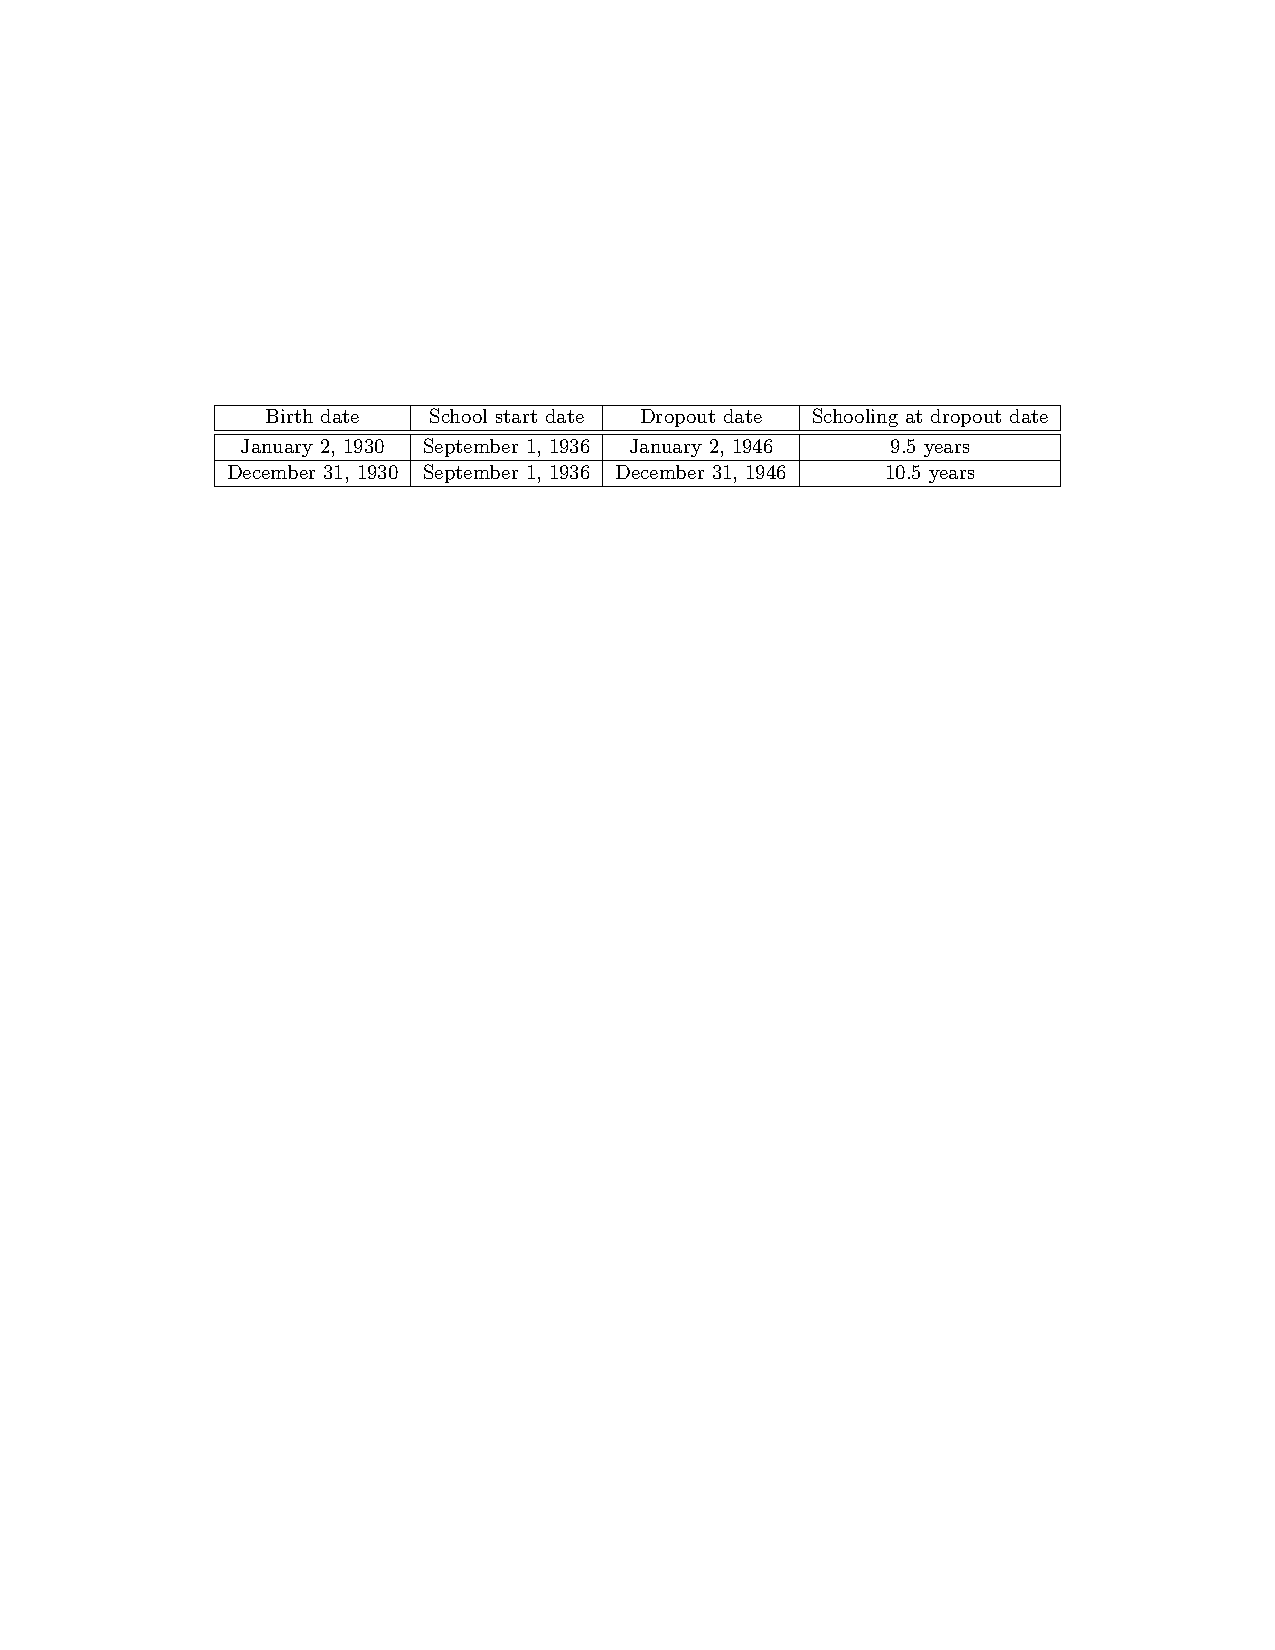
\includepdf{assets/6/qob_chart.pdf}
\begin{frame}{Angrist and Krueger (1991)}

\begin{itemize}
\item {\small{}The combination of dropout and age-at-entry rules means that
compulsory schooling requirements are higher for those born late in
the year\medskip{}
}{\small\par}
\item {\small{}This suggests an IV strategy using date of birth as an instrument
for schooling\medskip{}
}{\small\par}
\item {\small{}AK use a ``quarter of birth'' instrument, an indicator
for being born early in the year (January - March)\medskip{}
}{\small\par}
\item {\small{}What are the first stage and exclusion restriction assumptions
in this example?}{\small\par}
\end{itemize}
\end{frame}
\setbeamercolor{background canvas}{bg=} 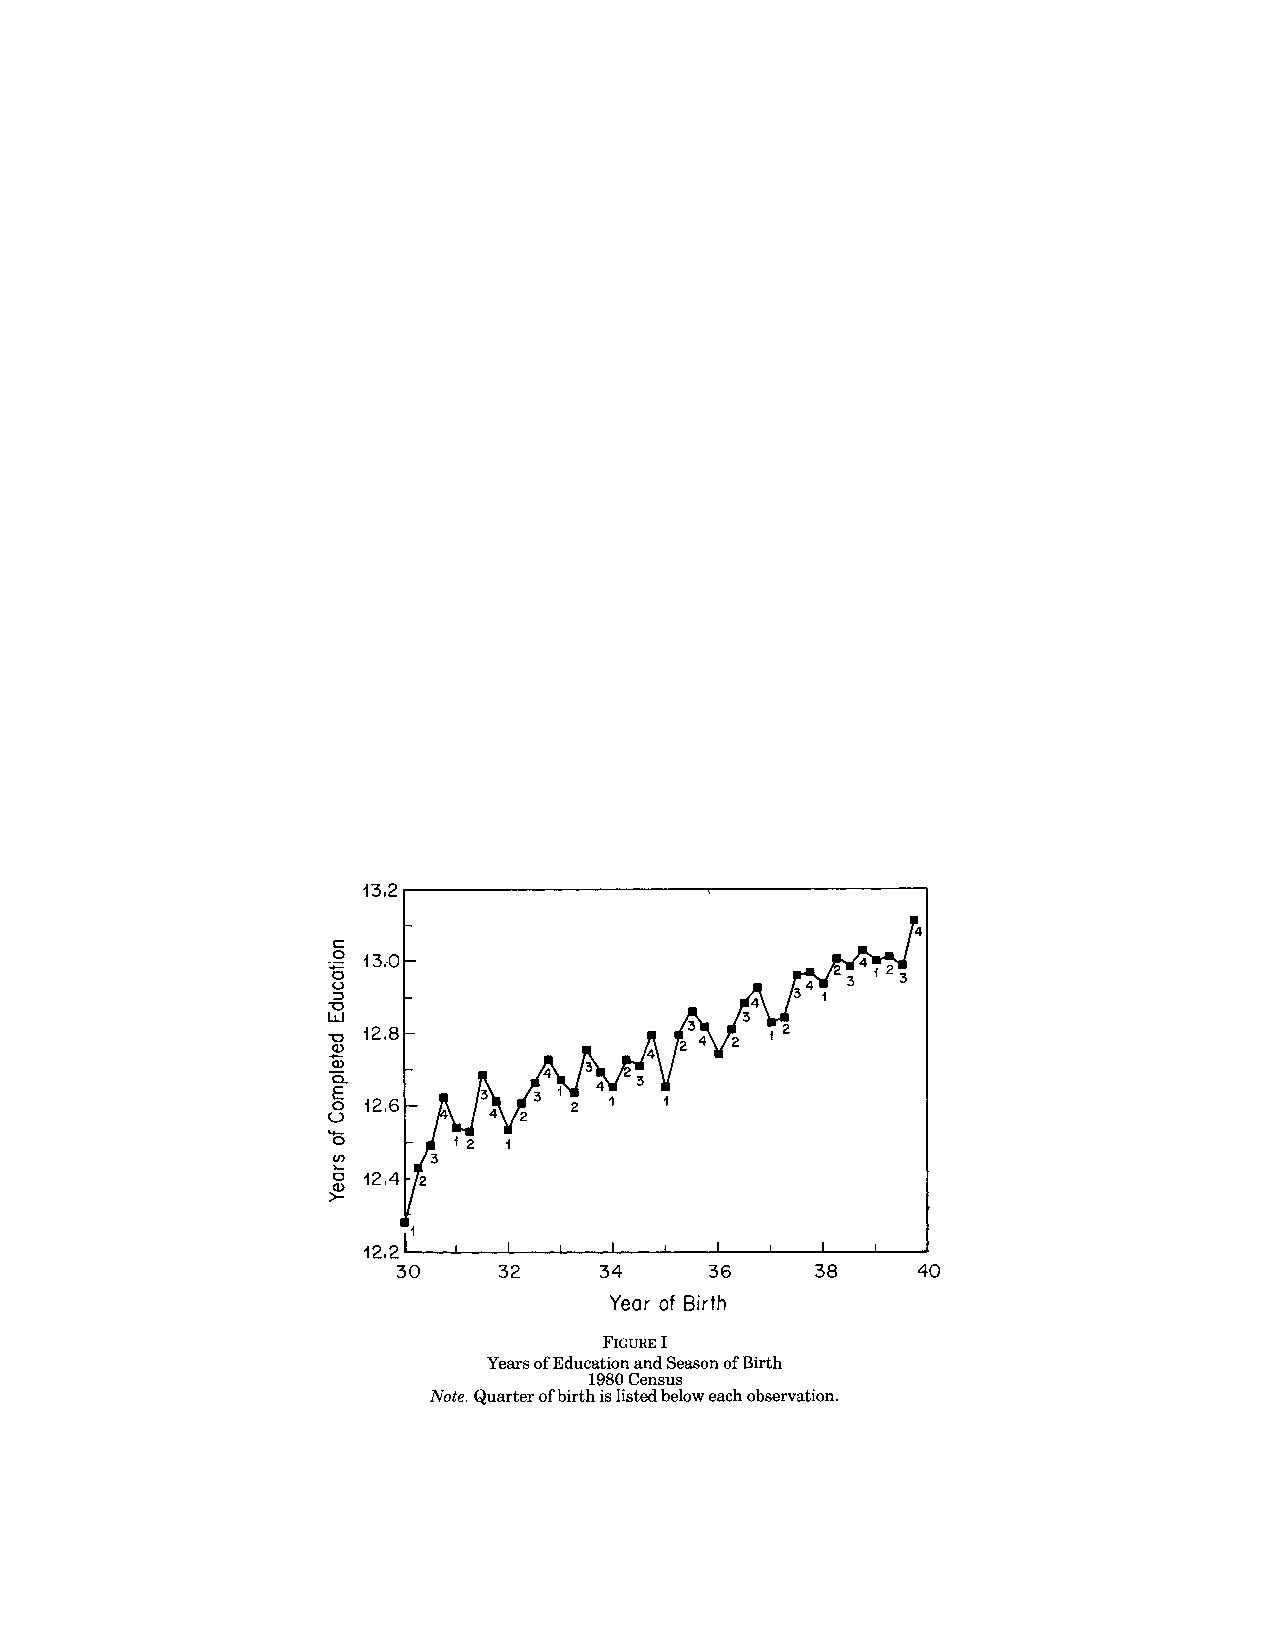
\includepdf{assets/6/angrist_kruger_1991_f1.pdf}

\setbeamercolor{background canvas}{bg=} 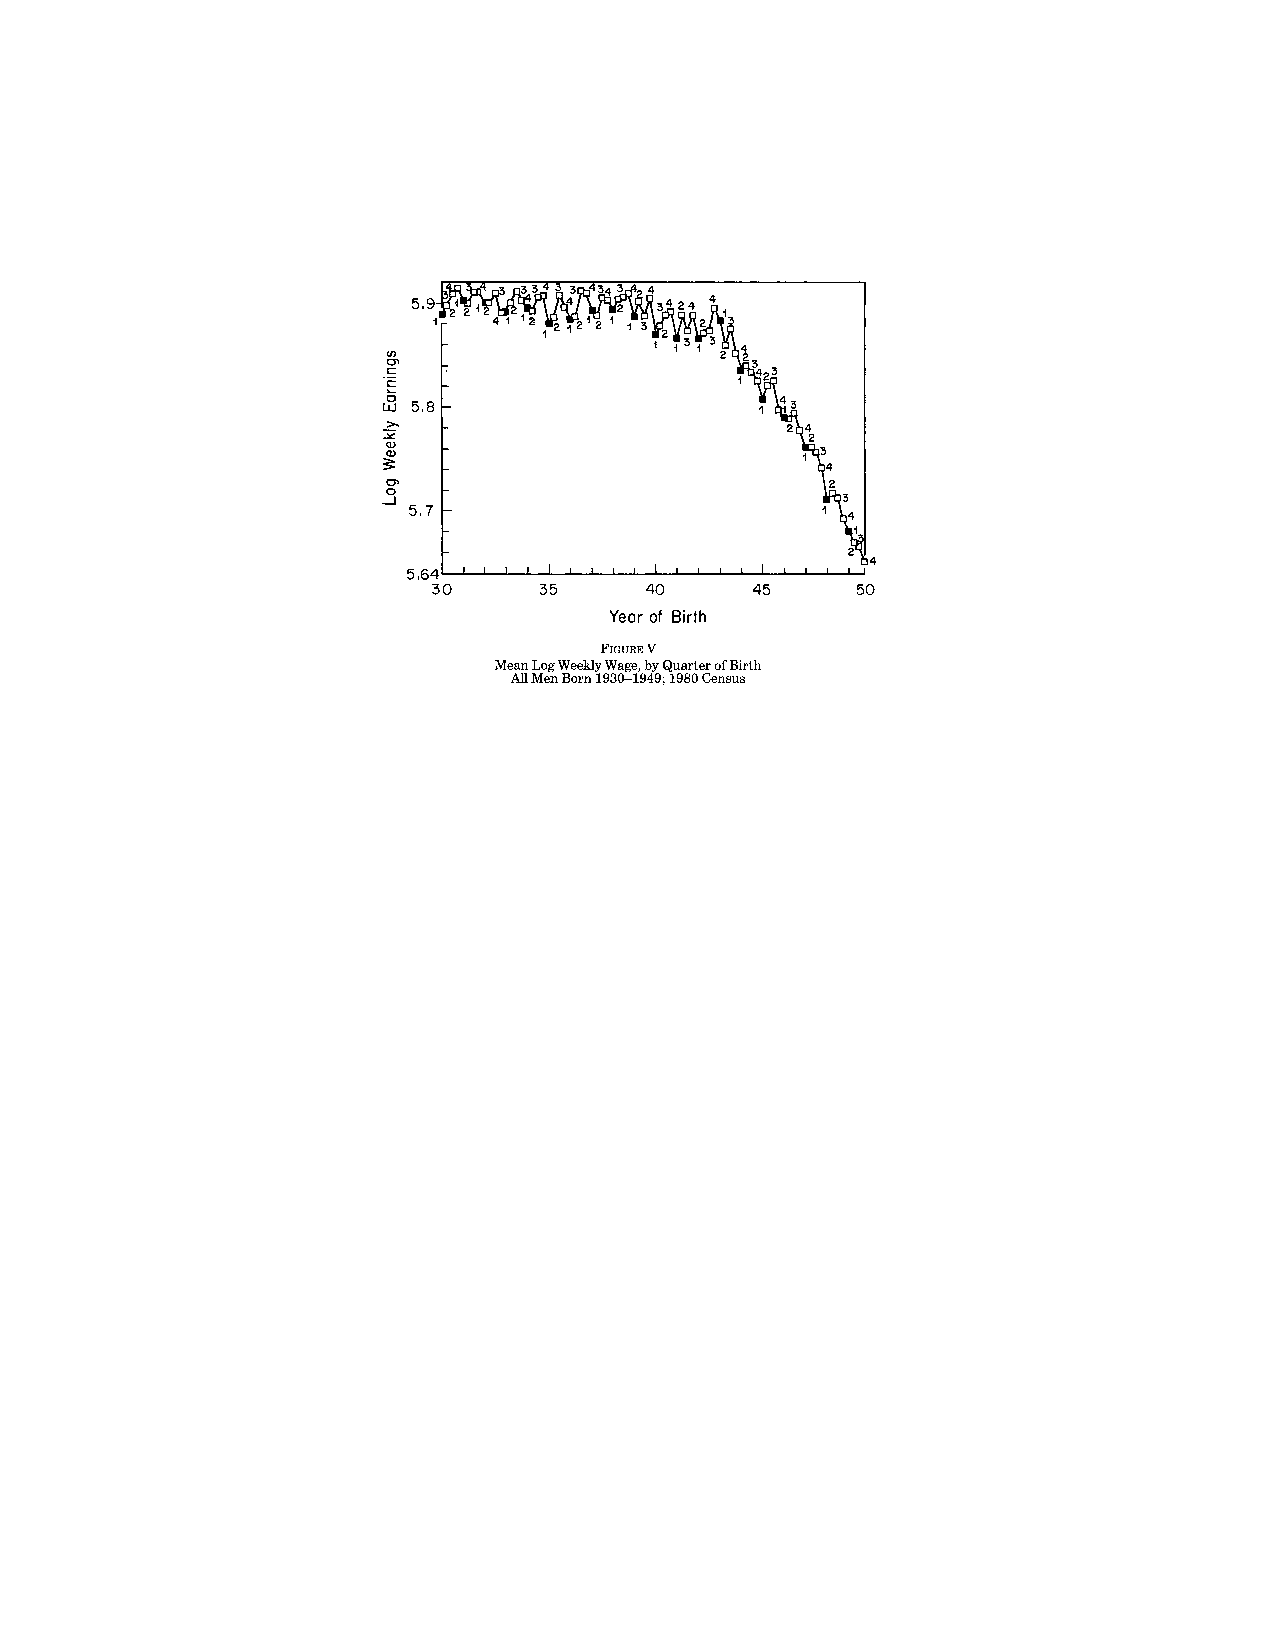
\includepdf{assets/6/angrist_krueger_1991_f5.pdf}
\begin{frame}{The Wald Estimator}

\begin{center}
$\rho_{IV}=\dfrac{Cov(Y_{i},Z_{i})/Var(Z_{i})}{Cov(S_{i},Z_{i})/Var(Z_{i})}$
\par\end{center}
\begin{itemize}
\item When $Z_{i}$ is binary, the first stage and reduced form coefficients
become differences in means:
\end{itemize}
\begin{center}
$\rho_{IV}=\dfrac{E\left[Y_{i}|Z_{i}=1\right]-E\left[Y_{i}|Z_{i}=0\right]}{E\left[S_{i}|Z_{i}=1\right]-E\left[S_{i}|Z_{i}=0\right]}$
\par\end{center}
\begin{itemize}
\item This is the population analogue of the Wald (1940) estimator, the
ratio of the mean difference in the outcome to the mean difference
in the endogenous regressor
\end{itemize}
\end{frame}
\setbeamercolor{background canvas}{bg=} 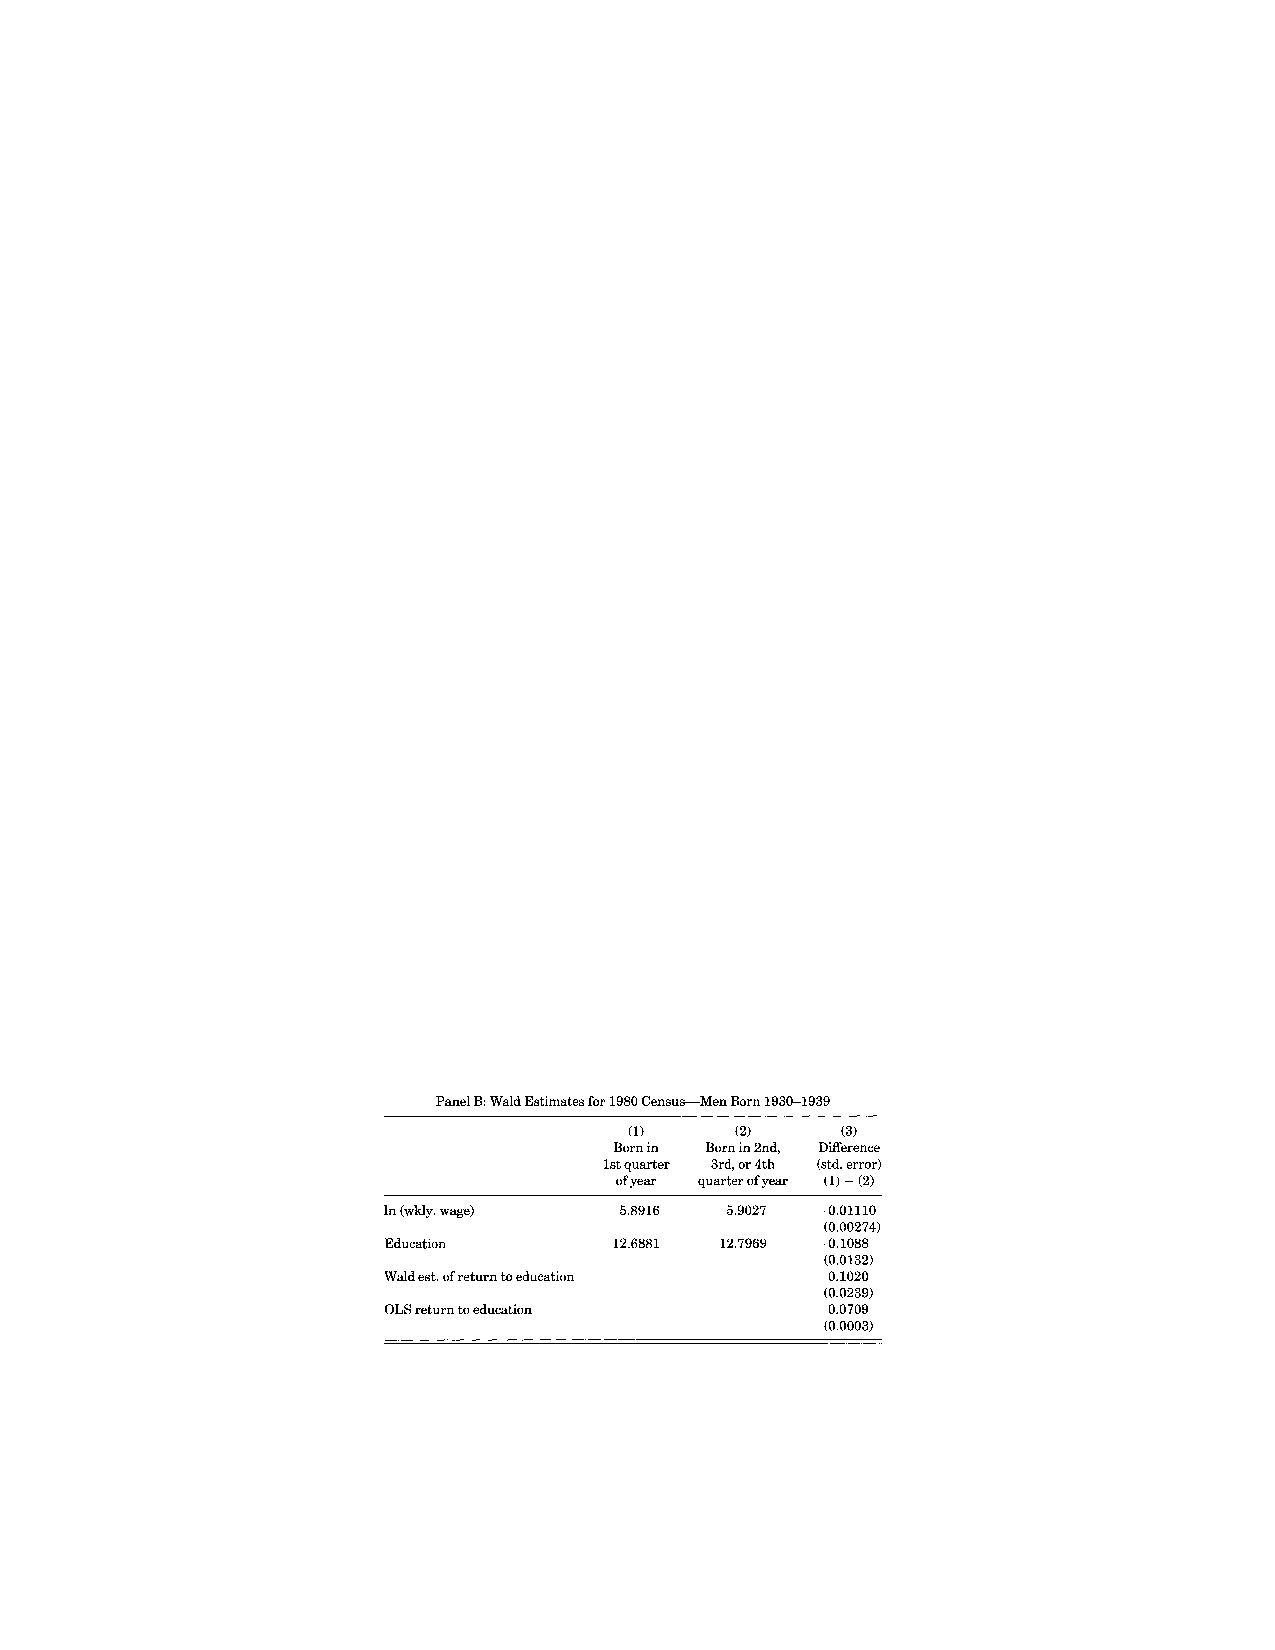
\includepdf{assets/6/angrist_krueger_1991_t3.pdf}

\begin{frame}{IV with Covariates}

\begin{itemize}
\item {\small{}When doing IV it's often necessary to control for additional
observed variables\medskip{}
}{\small\par}
\item {\small{}Example: QOB is correlated with age, which likely also affects
earnings. This suggests a violation of the exclusion restriction;
we may want to control for smooth functions of age\medskip{}
}{\small\par}
\item {\small{}The long regression of interest now includes the control
vector $X_{i}$:}{\small\par}
\end{itemize}
\begin{center}
{\small{}$Y_{i}=\alpha+\rho S_{i}+X_{i}^{\prime}\gamma+\gamma A_{i}+v_{i}$}{\small\par}
\par\end{center}
\begin{itemize}
\item {\small{}Control variables that are neither instruments nor instrumented
are ``exogenous covariates''}{\small\par}
\end{itemize}
\end{frame}

\begin{frame}{IV with Covariates}

\begin{itemize}
\item {\small{}Reduced form and first stage regressions augmented with covariates:}{\small\par}
\end{itemize}
\begin{center}
{\small{}$Y_{i}=\lambda+\delta Z_{i}+X_{i}^{\prime}\psi+u_{i}$}{\small\par}
\par\end{center}

\begin{center}
{\small{}$S_{i}=\kappa+\pi Z_{i}+X_{i}^{\prime}\phi+\eta_{i}$}{\small\par}
\par\end{center}
\begin{itemize}
\item {\small{}As before we can solve for $\rho$ as $\delta/\pi$\medskip{}
}{\small\par}
\item {\small{}Applying the Frisch-Waugh-Lovell theorem, this can be written}{\small\par}
\end{itemize}
\begin{center}
{\small{}$\dfrac{\delta}{\pi}=\dfrac{Cov\left(Y_{i},\tilde{Z}_{i}\right)}{Cov\left(S_{i},\tilde{Z}_{i}\right)}$}{\small\par}
\par\end{center}

\end{frame}

\begin{frame}{Indirect Least Squares}

\begin{center}
{\small{}$\dfrac{\delta}{\pi}=\dfrac{Cov\left(Y_{i},\tilde{Z}_{i}\right)}{Cov\left(S_{i},\tilde{Z}_{i}\right)}$}{\small\par}
\par\end{center}
\begin{itemize}
\item {\small{}The sample analogue of this ratio is called the Indirect
Least Squares (ILS) estimator \medskip{}
}{\small\par}
\item {\small{}Controlling for covariates is equivalent to using the residual
from a regression of $Z_{i}$ on $X_{i}$ as the instrument\medskip{}
}{\small\par}
\item {\small{}The first stage and exclusion restriction assumptions now
need to hold for $\tilde{Z}_{i}$ rather than $Z_{i}$\medskip{}
}{\small\par}
\item {\small{}Importantly, this means that the first stage relationship
between $S_{i}$ and $Z_{i}$ must survive the addition of the controls
$X_{i}$}{\small\par}
\end{itemize}
\end{frame}
\subsection{2SLS and Multiple Instruments}
\begin{frame}{Multiple Instruments }

\begin{itemize}
\item {\small{}Now suppose we have multiple instruments, $Z_{i1}...Z_{iJ}$,
collected in the $J\times1$ vector $Z_{i}$\medskip{}
}{\small\par}
\item {\small{}Example: dummies for each quarter of birth, rather than just
the first quarter\medskip{}
}{\small\par}
\item {\small{}It's no longer clear how to solve for the long regression
coefficient $\rho$. We could use any one of the $J$ instruments,
or any linear combination of them\medskip{}
}{\small\par}
\item {\small{}$\rho$ is now }\textbf{\small{}overidentified}{\small{}:
there are multiple ways to solve for the parameter of interest\medskip{}
}{\small\par}
\item {\small{}How should we combine the available information?}{\small\par}
\end{itemize}
\end{frame}

\begin{frame}{Multiple Instruments }

\begin{itemize}
\item {\small{}Our structural equation of interest is still }{\small\par}
\end{itemize}
\begin{center}
{\small{}$Y_{i}=\alpha+\rho S_{i}+X_{i}^{\prime}\gamma+\varepsilon_{i}$}{\small\par}
\par\end{center}
\begin{itemize}
\item {\small{}Consider a first-stage regression of $S_{i}$ on all the
instruments and exogenous controls:}{\small\par}
\end{itemize}
\begin{center}
{\small{}$S_{i}=\kappa+Z_{i}^{\prime}\pi+X_{i}^{\prime}\phi+\eta_{i}$}{\small\par}
\par\end{center}

\end{frame}

\begin{frame}{Multiple Instruments }

\begin{itemize}
\item {\small{}Substitute the first stage regression into the structural
equation:}{\small\par}
\end{itemize}
\begin{center}
{\small{}$Y_{i}=\alpha+\rho\left[\kappa+Z_{i}^{\prime}\pi+X_{i}^{\prime}\phi+\eta_{i}\right]+X_{i}^{\prime}\gamma+\varepsilon_{i}$}{\small\par}
\par\end{center}

\begin{center}
{\small{}$=\alpha+\rho\left(\kappa+Z_{i}^{\prime}\pi+X_{i}^{\prime}\phi\right)+X_{i}^{\prime}\gamma+\left(\rho\eta_{i}+\varepsilon_{i}\right)$}{\small\par}
\par\end{center}

\begin{center}
{\small{}$=\alpha+\rho\hat{S}_{i}+X_{i}^{\prime}\gamma+\nu_{i}$}{\small\par}
\par\end{center}
\begin{itemize}
\item {\small{}Here $\hat{S}_{i}=\kappa+Z_{i}^{\prime}\pi+X_{i}^{\prime}\phi$
is the predicted value of $S_{i}$ from the first stage\medskip{}
}{\small\par}
\item {\small{}The new residual is $\nu_{i}=\rho\eta_{i}+\varepsilon_{i}=\rho(S_{i}-\hat{S}_{i})+\varepsilon_{i}$}{\small\par}
\end{itemize}
\end{frame}

\begin{frame}{Two-Stage Least Squares}

\begin{center}
{\small{}$Y_{i}=\alpha+\rho\hat{S}_{i}+X_{i}^{\prime}\gamma+\nu_{i}$}{\small\par}
\par\end{center}
\begin{itemize}
\item {\small{}$\hat{S}_{i}$ and $X_{i}$ are uncorrelated with $\nu_{i}$
(why?), so OLS recovers the parameters of this equation\medskip{}
}{\small\par}
\item {\small{}This is the two-stage least squares (2SLS) estimator:\medskip{}
}

\begin{enumerate}
\item {\small{}Regress $S_{i}$ on all the instruments and exogenous controls,
and obtain predicted values $\hat{S}_{i}$\medskip{}
}{\small\par}
\item {\small{}Regress $Y_{i}$ on $\hat{S}_{i}$ and the exogenous controls\medskip{}
}{\small\par}
\end{enumerate}
\item {\small{}2SLS provides one method for combining instruments. Do you think it is the most efficient?}{\small\par}
\end{itemize}
\end{frame}
\subsection{IV as GMM}
\begin{frame}{IV Estimation}

\begin{itemize}
\item {\small{}Suppose we have $N$ observations on $(Y_{i},S_{i},Z_{i},X_{i})$,
where \medskip{}
}

\begin{itemize}
\item {\small{}$S_{i}$ is a $K\times1$ vector of endogenous variables
(there now may be more than one)\medskip{}
}{\small\par}
\item {\small{}$Z_{i}$ is a $J\times1$ vector of instruments\medskip{}
}{\small\par}
\item {\small{}$X_{i}$ is an $L\times1$ vector of exogenous controls\medskip{}
}{\small\par}
\end{itemize}
\item {\small{}Let $\mathbf{X}_{i}=\left(1,X_{i}^{\prime},S_{i}^{\prime}\right)^{\prime}$
and $\mathbf{Z}_{i}=(1,X_{i}^{\prime},Z_{i}^{\prime})^{\prime}$}{\small\par}
\end{itemize}
\end{frame}


\begin{frame}{IV as GMM}
\begin{itemize}
\item {\small{}Let's augment our structural equation}{\small\par}
\begin{center}
{\small{}$Y_{i}=\alpha+S_{i}^{\prime}\rho+X_{i}^{\prime}\gamma+\varepsilon_{i}$}{\small\par}
\par\end{center}
\begin{itemize}
\item {\small{}$S_{i}$ is a $K\times1$ vector of endogenous variables
(there now may be more than one)\medskip{}
}{\small\par}
\item {\small{}$Z_{i}$ is a $J\times1$ vector of instruments ($J\geq K$)\medskip{}
}{\small\par}
\item {\small{}$X_{i}$ is an $L\times1$ vector of exogenous controls\medskip{}
}{\small\par}
\item {\small{}Let $\mathbf{X}_{i}=\left(1,X_{i}^{\prime},S_{i}^{\prime}\right)^{\prime}$
and $\mathbf{Z}_{i}=(1,X_{i}^{\prime},Z_{i}^{\prime})^{\prime}$}{\small\par}
\end{itemize}
\pause
\item We know (from either economic theory or institutional knowledge of $Z_{i}$ and $S_{i}$) that 
\be
\E[\mathbf{Z}_{i}'\varepsilon_{i}]=\E[\mathbf{Z}_{i}'(y_{i}-\alpha-S_{i}^{\prime}\rho-X_{i}^{\prime}\gamma)]=\E[m_{i}(\theta)]=0
\ee
where $\theta=(\rho;\gamma)$
\item What do we call this? How many equations? How many unknowns?
\end{itemize}
\end{frame}
%%
\begin{frame}
\frametitle{Casting everything as GMM}
\begin{itemize}
\item Recall previous class on GMM (see Estimation slide deck). GMM minimizes the following criterion function
\be
\label{GMM_criterion}
Q_{GMM}(\theta)=\E[m_{i}(\theta)'\mathbf{W} m_{i}(\theta)] 
\ee
\item What happens to $\mathbf{W}$ when $J=K$? 
\medskip
\pause
\item How do we choose $\mathbf{W}$ when $J>K$?
\pause
\medskip
\item Turns out that 2SLS minimizes \eqref{GMM_criterion} by setting $\mathbf{W}=E[\mathbf{Z}_{i}\mathbf{Z}_{i}']^{-1}$ $\rightarrow$ When is 2SLS efficient? {\tiny{See Section 4.2.1 of MHE for full proof.}}
\pause
\medskip
\item What is the optimal $\mathbf{W}$ in a general setup?
\pause
\medskip
\item Efficient GMM: $\mathbf{W}^{*}=\boldsymbol{\Omega}^{-1}$, where $\boldsymbol{\Omega}=\E[m_{i}(\theta)m_{i}(\theta)']=\E[\varepsilon_{i}^{2}\mathbf{Z}_{i}\mathbf{Z}_{i}']$
\begin{itemize}
\item Under homoskedasticity, $\E[\varepsilon_{i}^{2}|\mathbf{Z}_{i}]=\sigma^{2}$, so $\boldsymbol{\Omega}^{-1}=\sigma^{-2}\E[\mathbf{Z}_{i}\mathbf{Z}_{i}']^{-1}\propto$ the 2SLS weight $\rightarrow$ 2SLS is efficient
\item With heteroskedasticity, $\boldsymbol{\Omega}$ must be estimated: $\hat{\boldsymbol{\Omega}}=\frac{1}{N}\sum_{i}\hat{\varepsilon}_{i}^{2}\mathbf{Z}_{i}\mathbf{Z}_{i}'$ using 2SLS residuals (two-step GMM)
\end{itemize}
\end{itemize}
\end{frame}
%%
%%
\subsection{Overidentification Tests}
\begin{frame}
\frametitle{Over-id Test}
\begin{itemize}
\item GMM formulation also useful to think on how we can test the validity of the ``model". 
\medskip
\item When there are more instruments than endogenous variables ($J>K$) there are multiple ways to solve for the structural parameters. 
\medskip
\item Essentially an over-id specification test (as introduced in the Estimation slide-deck) tells us how close to being satisfied the moment condition are. 
\medskip
\item In the IV setup, this means that an overid test checks whether \textit{all} the IV moment restrictions are close enough to being satisfied. 
\end{itemize}
\end{frame}
%%
\begin{frame}
\frametitle{Overid Tests in the IV world}
\begin{itemize}
\item Let $\hat{\theta}$ be the minimizer of the sample GMM criterion function 
\be
\label{GMM_sample_criterion}\hat{\theta}=\argmin_{c}\hat{Q}_{GMM}(c)=N\hat{m}_{i}(c)'\mathbf{W} \hat{m}_{i}(c) 
\ee
where $\hat{m}_{i}(\theta)=\dfrac{1}{N}\mathbf{Z}_{i}'(y_{i}-\alpha-S_{i}^{\prime}\rho-X_{i}^{\prime}\gamma)$ (evaluated at the ``truth" $\theta$)
\medskip
\item If $\mathbf{W}= \E[\sqrt{N}\hat{m}_{i}(\theta)\sqrt{N}\hat{m}_{i}(\theta)']^{-1}$, then as $N\rightarrow \infty$
\medskip
\be
\hat{Q}_{GMM}(\hat{\theta})\sim\chi^{2}_{J-K}
\ee
(sometimes this is also called the J-test in the IV setup).
\medskip
\item If $\hat{Q}_{GMM}(\hat{\theta})$ is large relative to critical value of $\chi^{2}_{J-K}$ $\rightarrow$ model is rejected. 
\medskip
\item Rejection means that one of the $J$ instrument is false, i.e. there is one instrument for which $\E[Z_{i}\varepsilon_{i}]$ is actually not zero!
\end{itemize}
\end{frame}
%%
\begin{frame}
\frametitle{Intuition}

\begin{itemize}
\item Suppose that there are no controls and we have one endogenous variable $S_{i}$ and two potential instruments $Z_{i1}$ and $Z_{i2}$.  
\medskip
\item Two instruments give us two potential (simple) IV estimates of $\rho$. 
\medskip 
\item First estimate of $\rho$ obtained by solving moment condition 
\be
\E[Z_{i1}(y_{i}-S_{i}\rho_{1})]=0
\ee 
\item And the second one is obtained by fitting 
\be
\E[Z_{i2}(y_{i}-S_{i}\rho_{2})]=0
\ee
\pause
\item Over-id tests whether a model that imposes $\rho_{2}=\rho_{1}$ can fit the data. 
\medskip
\item What is the key underlying assumption that we need to make this test truly useful?
\end{itemize}
\end{frame}
\subsection{Imperfect Compliance}
\begin{frame}{Which research questions can be answered causally?}
\begin{itemize}
    \item Go back to our discussion we had in the first class: often times economists are interested in the causal effect of \textit{choices} made by agents (e.g. attend a private university, smoking, do a pre-cancer screening test, etc).
    \medskip
    \item The gold standard in research is the RCT but sometimes you can't randomize individuals into treatment (IRB won't allow it and for very good reasons).
    \medskip
    \item Strategy is then to randomize $Z_{i}$ where $Z_{i}$ is some incentive to take up a given treatment of interest, $D_{i}$.
    \medskip
    \item Even if there is imperfect compliance $\Pr(D_{i}=1| Z_{i}=1)\neq 1$ one can use IV techniques to estimate a causal effect. 
    \medskip
    \item Simple but powerful idea that still needs to make its way in \textit{all} fields...   
\end{itemize}
\end{frame}
\begin{frame}{IV Makes Its Way in Clinical Trials}
\begin{itemize}
    \item RQ: do pre-cancer screenings improve health?
    \medskip
    \item Can't force doctors (or patients) to test so people have tried to answer this question by randomizing the opportunity to screen... 
    \medskip
    \item Studies in this area thus report Intention-to-Treat (or Intention-to-Screen) Effects: $\E[Y_{i}\vert Z_{i}=1]-\E[Y_{i}\vert Z_{i}=0]$.
    \medskip
    \item There seems to be a lot of heterogeneity in the ITTs estimated across a whole variety of studies 
    \medskip
    \item Winawer (2023) asks ``are these intention-to-treat observations applicable to other
clinical environments?"   
\end{itemize}
\end{frame}
\begin{frame}[plain]

\begin{center}
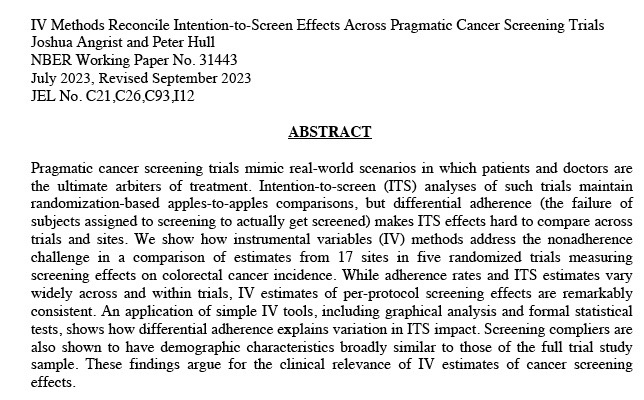
\includegraphics[scale=0.4]{assets/6/angrist_hull_IV_1}
\par\end{center}


\end{frame}
\begin{frame}[plain]

\begin{center}
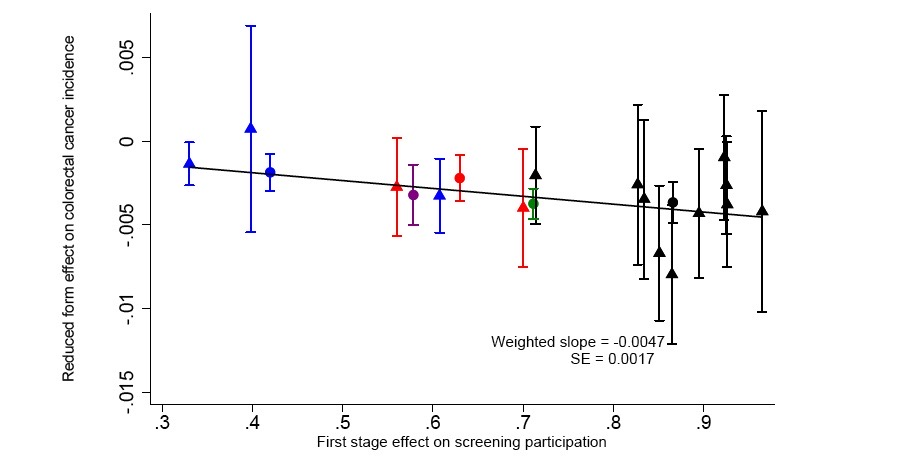
\includegraphics[scale=0.4]{assets/6/angrist_hull_IV_0}
\par\end{center}


\end{frame}
\begin{frame}[plain]

\begin{center}
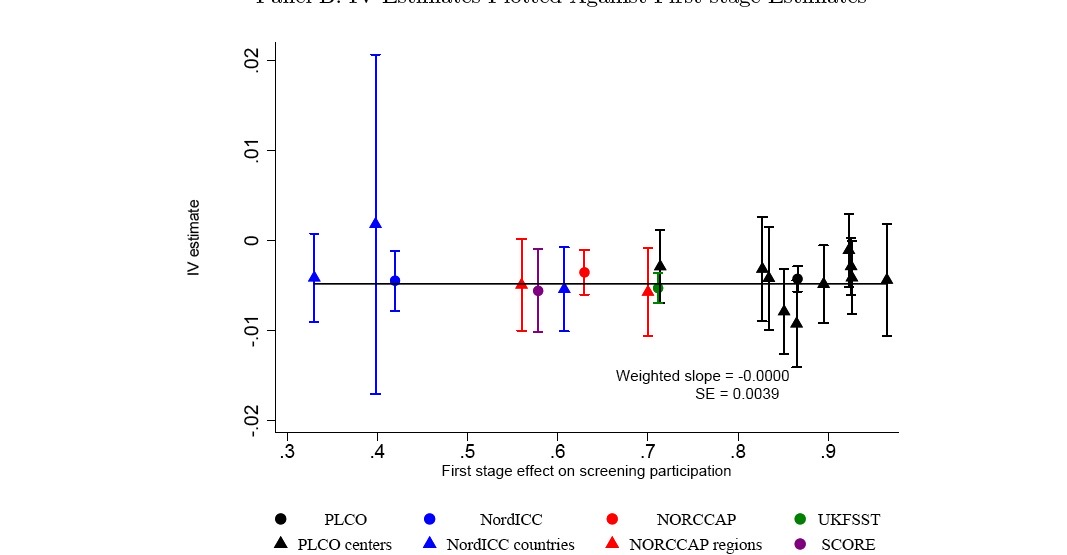
\includegraphics[scale=0.3]{assets/6/angrist_hull_IV_2}
\par\end{center}


\end{frame}

\subsection{2SLS Mistakes}
\begin{frame}{2SLS Mistakes}

\begin{itemize}
\item {\small{}2SLS is the workhorse IV estimator used by empirical researchers\medskip{}
}{\small\par}
\item {\small{}It's worth covering some common pitfalls related to 2SLS
estimation}{\small\par}
\end{itemize}
\end{frame}

\begin{frame}{2SLS Mistakes 1: Standard Errors}

\begin{itemize}
\item {\small{}It's usually not a good idea to run the two stages of 2SLS
manually\medskip{}
}{\small\par}
\item {\small{}For one thing, this will give the wrong standard errors\medskip{}
}{\small\par}
\item {\small{}Consider a setting with one endogenous variable $S_{i}$}{\small\par}
\end{itemize}
\begin{center}
{\small{}$Y_{i}=\alpha+\rho S_{i}+\varepsilon_{i}$}{\small\par}
\par\end{center}
\begin{itemize}
\item {\footnotesize{}If you run 2SLS manually, the second stage is}{\footnotesize\par}
\end{itemize}
\begin{center}
{\footnotesize{}$Y_{i}=\alpha+\rho\hat{S}_{i}+v_{i}$}{\footnotesize\par}
\par\end{center}
\begin{itemize}
\item {\footnotesize{}Here $v_{i}=\varepsilon_{i}+\rho(S_{i}-\hat{S}_{i})$\medskip{}
}{\footnotesize\par}
\end{itemize}
\begin{itemize}
\item {\footnotesize{}Manual 2SLS will typically generate standard errors
that are too large.
\medskip{}
}{\footnotesize\par}
\item {\footnotesize{}The residual variance should be calculated from the
structural residual $Y_{i}-\hat{\alpha}-\hat{\rho}S_{i}$, not the
second-stage residual $Y_{i}-\hat{\alpha}-\hat{\rho}\hat{S}_{i}$}{\footnotesize\par}
\end{itemize}
\end{frame}

\begin{frame}{2SLS Mistakes 2: Covariate Ambivalence}

\begin{itemize}
\item {\small{}A second possible mistake in manual 2SLS is the treatment
of covariates\medskip{}
}{\small\par}
\item {\small{}Suppose we run the 2SLS procedure}{\small\par}
\end{itemize}
\begin{center}
{\small{}$S_{i}=\kappa+Z_{i}^{\prime}\pi+X_{1i}^{\prime}\phi_{1}+\eta_{i}$}{\small\par}
\par\end{center}

\begin{center}
{\small{}$Y_{i}=\alpha+\rho\hat{S}_{i}+X_{1i}^{\prime}\theta_{1}+X_{2i}^{\prime}\theta_{2}+v_{i}$}{\small\par}
\par\end{center}
\begin{itemize}
\item {\small{}The covariate vector $X_{2i}$ is included in the second
stage but not the first (the opposite of the instruments $Z_{i}$)\medskip{}
}{\small\par}
\item {\small{}What's wrong with this?}{\small\par}
\end{itemize}
\end{frame}

\begin{frame}{2SLS Mistakes 2: Covariate Ambivalence}

\begin{center}
{\small{}$S_{i}=\kappa+Z_{i}^{\prime}\pi+X_{1i}^{\prime}\phi_{1}+\eta_{i}$}{\small\par}
\par\end{center}

\begin{center}
{\small{}$Y_{i}=\alpha+\rho\hat{S}_{i}+X_{1i}^{\prime}\theta_{1}+X_{2i}^{\prime}\theta_{2}+v_{i}$}{\small\par}
\par\end{center}
\begin{itemize}
\item {\small{}The second-stage residual is $v_{i}=\varepsilon_{i}+\rho(S_{i}-\hat{S}_{i})$\medskip{}
}{\small\par}
\item {\small{}Since $S_{i}-\hat{S}_{i}$ is a residual from a regression
that includes $X_{1i},$ $Cov(X_{1i},S_{i}-\hat{S}_{i})=0$\medskip{}
}{\small\par}
\item {\small{}But in general $Cov(S_{i}-\hat{S}_{i},X_{2i})\neq0$, so
we may have created a correlation between the error term and covariates,
leading to bias in all parameter estimates\medskip{}
}{\small\par}
\item {\small{}``If a covariate is good enough for the second stage, it's
good enough for the first.''}{\small\par}
\end{itemize}
\end{frame}

\begin{frame}{2SLS Mistakes 3: The Forbidden Regression}

\begin{itemize}
\item {\small{}In response to repeated mistakes by graduate students, Jerry
Hausman labeled one 2SLS mistake ``the forbidden regression'' \medskip{}
}{\small\par}
\item {\small{}The forbidden regression involves the erroneous application
of 2SLS logic to nonlinear models\medskip{}
}{\small\par}
\item {\small{}Suppose there is a dummy endogenous variable $T_{i}\in\{0,1\}$,
a vector of covariates $X_{i}$ and a vector of instruments $Z_{i}$\medskip{}
}{\small\par}
\item {\small{}The causal equation is}{\small\par}
\end{itemize}
\begin{center}
$Y_{i}=\alpha+\rho T_{i}+X_{i}^{\prime}\theta+\varepsilon_{i}$
\par\end{center}

\end{frame}

\begin{frame}{2SLS Mistakes 3: The Forbidden Regression}

\begin{itemize}
\item {\small{}First stage regression:}{\small\par}
\end{itemize}
\begin{center}
{\small{}$T_{i}=\kappa+Z_{i}^{\prime}\pi+X_{i}^{\prime}\phi+\eta_{i}$}{\small\par}
\par\end{center}
\begin{itemize}
\item {\small{}Since $T_{i}$ is binary, $E\left[T_{i}|Z_{i},X_{i}\right]$
is likely nonlinear unless the model is saturated. The first stage
is therefore a misspecified model of the CEF \medskip{}
}{\small\par}
\item {\small{}One might be tempted to try a nonlinear model to better approximate
the CEF, e.g. a probit:}{\small\par}
\end{itemize}
\begin{center}
{\small{}$Pr\left[T_{i}=1|X_{i},Z_{i}\right]=\Phi\left(\kappa+Z_{i}^{\prime}\pi+X_{i}^{\prime}\phi\right)$}{\small\par}
\par\end{center}

\end{frame}

\begin{frame}{2SLS Mistakes 3: The Forbidden Regression}

\begin{itemize}
\item {\small{}The nonlinear first stage can be used to obtain predicted
values:}{\small\par}
\end{itemize}
\begin{center}
{\small{}$\hat{T}_{i}=\Phi\left(\hat{\kappa}+Z_{i}^{\prime}\hat{\pi}+X_{i}^{\prime}\hat{\phi}\right)$}{\small\par}
\par\end{center}
\begin{itemize}
\item {\small{}One might then be tempted to run a 2SLS-style second stage:}{\small\par}
\end{itemize}
\begin{center}
{\small{}$Y_{i}=\alpha+\rho\hat{T}_{i}+X_{i}^{\prime}\theta+\varepsilon_{i}$$ $}{\small\par}
\par\end{center}
\begin{itemize}
\item {\small{}This regression is forbidden!}{\small\par}
\end{itemize}
\end{frame}

\begin{frame}{2SLS Mistakes 3: The Forbidden Regression}

\begin{itemize}
\item {\footnotesize{}To see why the forbidden regression is forbidden,
rewrite the structural equation}{\footnotesize\par}
\end{itemize}
\begin{center}
{\footnotesize{}$Y_{i}=\alpha+\rho\hat{T}_{i}+X_{i}^{\prime}\theta+\left(\varepsilon_{i}+\rho(T_{i}-\hat{T}_{i})\right)$}{\footnotesize\par}
\par\end{center}
\begin{itemize}
\item {\footnotesize{}If the first stage is estimated via OLS, then the
residual $(T_{i}-\hat{T}_{i})$ is guaranteed to be uncorrelated with
the fit $\hat{T}_{i}$ and with the included covariates $X_{i}$\medskip{}
}{\footnotesize\par}
\item {\footnotesize{}Nonlinear residuals do not have this property. $Cov\left(T_{i}-\hat{T}_{i},\hat{T}_{i}\right)$
and $Cov\left(T_{i}-\hat{T}_{i},X_{i}\right)$ will generally only
equal zero when the $E\left[T_{i}|X_{i},Z_{i}\right]$ is really a
probit\medskip{}
}{\footnotesize\par}
\item {\footnotesize{}Who knows whether the probit CEF is right? Better
to stick with a linear first stage, which guarantees zero covariance
between residuals and fits/regressors even if the CEF is misspecified}{\footnotesize\par}
\end{itemize}
\end{frame}
\begin{frame}
\frametitle{Pop-Quiz}
\pause
\begin{itemize}
\item Suppose you came up with what you think is a good instrument, $Z_{i}$.
\medskip
\item You are however not 100\% sure about the exclusion restriction.
\medskip
\item Inspired by your knowledge of regression and the meaning of the exclusion restriction you come up with the following test for the validity of the instrument
\be
y_{i}=\alpha + \beta S_{i} + \gamma Z_{i} + r_{i}
\ee
\item That is you run a regression on your endogenous variable $S_{i}$ and the instrument $Z_{i}$. 
\medskip
\item Since the instrument only operates through the endogenous variable $S_{i}$, you argue that if the exclusion restriction is valid, then $\beta=\rho$ (the true casual effect) and $\gamma=0$.
\medskip
\item Right? Wrong?
\end{itemize}
\end{frame}

\subsection{Many/Weak Instruments}
\begin{frame}{Many/Weak Instruments: The Problem}
\begin{itemize}
\item \small OLS is unbiased in finite samples (linear CEF or fixed regressors). IV is not: it is a ratio of reduced form and first stage,
\[
E\left[\hat{\rho}_{IV}\right]=E\left[\dfrac{\hat{\delta}}{\hat{\pi}}\right]\neq\dfrac{E[\hat{\delta}]}{E[\hat{\pi}]}=\rho
\]
\item \small Just-identified IV: a ratio of two (jointly normal) estimates $\rightarrow$ no moments and fat tails (Cauchy as $\pi\rightarrow0$), but approximately \emph{median} unbiased: $Q_{0.5}(\hat{\rho}_{IV})\approx\rho$
\medskip
\item \small Overidentified 2SLS is worse: it is centered in the wrong place, \textbf{biased towards OLS}
\medskip
\item \small The bias grows with the number of instruments (overfitting the first stage) and as the first stage gets weaker $\rightarrow$ ``many/weak'' instruments
\medskip
\item \small Bound, Jaeger and Baker (1995) showed this matters in practice
\end{itemize}
\end{frame}

\begin{frame}{Bound, Jaeger and Baker (1995)}
\begin{itemize}
\item \small BJB revisit the Angrist and Krueger QOB instrument
\medskip
\item \small The Wald estimates we studied are just-identified, so the many/weak critique does not apply to them (a common misconception)
\medskip
\item \small But AK also report 2SLS estimates that add QOB $\times$ year-of-birth (30) and QOB $\times$ state-of-birth (150) interactions as instruments $\rightarrow$ overidentified by 179
\begin{itemize}
\item \footnotesize Rationale: compulsory schooling laws differ across states and cohorts
\item \footnotesize Asymptotically this can only help: better first-stage fit, smaller standard errors
\end{itemize}
\medskip
\item \small The QOB first stage is small and most interactions are irrelevant, so this is a severe many/weak scenario
\medskip
\item \small BJB's experiment: replace QOB with \textbf{randomly generated fake QOB}, which has no first stage by construction, and re-run AK's 2SLS
\end{itemize}
\end{frame}

\begin{frame}{Bound, Jaeger and Baker (1995)}
\begin{center}
{\footnotesize{}}%
\begin{tabular}{|c|c|c|c|}
\hline 
 & {\footnotesize{}2SLS (real QOB)} & {\footnotesize{}2SLS (fake QOB)} & {\footnotesize{}OLS}\tabularnewline
\hline 
\hline 
{\footnotesize{}30 QOB{*}year} & {\footnotesize{}0.081} & {\footnotesize{}0.062} & {\footnotesize{}0.063}\tabularnewline
\hline 
{\footnotesize{}interactions} & {\footnotesize{}(0.016)} & {\footnotesize{}(0.037)} & {\footnotesize{}(0.000)}\tabularnewline
\hline 
 &  &  & \tabularnewline
\hline 
{\footnotesize{}180 QOB{*}year and state} & {\footnotesize{}0.083} & {\footnotesize{}0.060} & {\footnotesize{}0.063}\tabularnewline
\hline 
{\footnotesize{}interactions} & {\footnotesize{}(0.009)} & {\footnotesize{}(0.015)} & {\footnotesize{}(0.000)}\tabularnewline
\hline 
\end{tabular}{\footnotesize\par}
\par\end{center}
\medskip
\begin{itemize}
\item \small With junk instruments, 2SLS essentially reproduces OLS
\medskip
\item \small Conventional standard errors give no warning: the fake-QOB, 180-instrument estimate looks precise despite having no first stage
\medskip
\item \small Where does this bias come from, and how do we diagnose and correct it?
\end{itemize}
\end{frame}

\begin{frame}{Where the Bias Comes From: Setup}
\begin{itemize}
\item \small One endogenous regressor, $Q$ instruments, in matrix form:
\begin{align*}
\text{Second stage:}\qquad & Y=\rho S+\varepsilon\\
\text{First stage:}\qquad & S=Z\pi+\eta
\end{align*}
\item \small 2SLS regresses $Y$ on $\hat{S}=P_{Z}S$, so
\[
\hat{\rho}_{2SLS}-\rho=(S'P_{Z}S)^{-1}S'P_{Z}\varepsilon=(S'P_{Z}S)^{-1}\left[\pi'Z'\varepsilon+\eta'P_{Z}\varepsilon\right]
\]
\pause
\item \small We want the expectation of this. Problem: $(S'P_{Z}S)^{-1}$ is random and correlated with the bracket (why?)
\medskip
\item \small Bekker (1994): under asymptotics where $Q$ grows with $N$, replacing $(S'P_{Z}S)^{-1}$ by $(E[S'P_{Z}S])^{-1}$ is a good approximation
\[
E\left[\hat{\rho}_{2SLS}-\rho\right]\approx\left(E[S'P_{Z}S]\right)^{-1}E\left[\pi'Z'\varepsilon+\eta'P_{Z}\varepsilon\right]
\]
\end{itemize}
\end{frame}

\begin{frame}{Where the Bias Comes From: The Trace Trick}
Condition on $Z$ and take the numerator one term at a time:
\begin{itemize}
\medskip
\item \small First term: $E[\pi'Z'\varepsilon\,|\,Z]=\pi'Z'E[\varepsilon\,|\,Z]=0$ (why?)
\pause
\medskip
\item \small Second term:
\begin{align*}
E[\eta'P_{Z}\varepsilon\,|\,Z] & =E\left[\mathrm{tr}(\eta'P_{Z}\varepsilon)\,|\,Z\right]=E\left[\mathrm{tr}(P_{Z}\varepsilon\eta')\,|\,Z\right]\\
 & =\mathrm{tr}\left(P_{Z}\,E[\varepsilon\eta'\,|\,Z]\right)=\sigma_{\eta\varepsilon}\,\mathrm{tr}(P_{Z})=\sigma_{\eta\varepsilon}\,Q
\end{align*}
%using $E[\varepsilon\eta'\,|\,Z]=\sigma_{\eta\varepsilon}I$ and $\mathrm{tr}(P_{Z})=\mathrm{tr}\left((Z'Z)^{-1}Z'Z\right)=Q$
\pause
\medskip
\item \small Uses two tricks: a scalar equals its trace, the trace is cyclic
\item \small (also relies on IID residual, can be adapted)
\item \small Nonzero because $\eta$ and $\varepsilon$ are correlated (why?)
\begin{itemize}
\item \small Intuition: each instrument lets $\hat{S}$ pick up a bit of $\eta$, hence of $\varepsilon$. More instruments, more leakage
\end{itemize}
\end{itemize}
\end{frame}

\begin{frame}{The Many/Weak Bias Formula}
\begin{itemize}
\item \small Same trick on the denominator: $E[S'P_{Z}S]=E[\pi'Z'Z\pi]+E[\eta'P_{Z}\eta]=E[\pi'Z'Z\pi]+\sigma_{\eta}^{2}\,Q$. Hence
\[
E\left[\hat{\rho}_{2SLS}-\rho\right]\approx\dfrac{\sigma_{\eta\varepsilon}\,Q}{E[\pi'Z'Z\pi]+\sigma_{\eta}^{2}\,Q}=\dfrac{\sigma_{\eta\varepsilon}}{\sigma_{\eta}^{2}}\cdot\dfrac{1}{1+F},\qquad F\equiv\dfrac{E[\pi'Z'Z\pi]}{\sigma_{\eta}^{2}\,Q}
\]
where $F$ is the population first-stage $F$-statistic for the joint significance of the instruments
\end{itemize}
\end{frame}

\begin{frame}{Comparing to OLS}
\begin{itemize}
\item \small Let $V\equiv Var(Z_{i}'\pi)$. OLS regresses $Y$ on $S$, and $Var(S_{i})=V+\sigma_{\eta}^{2}$, so
\[
\text{OLS bias}=\dfrac{Cov(S_{i},\varepsilon_{i})}{Var(S_{i})}=\dfrac{\sigma_{\eta\varepsilon}}{V+\sigma_{\eta}^{2}}
\]
\pause
\item \small Rewrite what we just derived in these terms:
\[
E\left[\hat{\rho}_{2SLS}-\rho\right]\approx\dfrac{\sigma_{\eta\varepsilon}}{\sigma_{\eta}^{2}}\cdot\dfrac{1}{1+F}=\dfrac{\sigma_{\eta\varepsilon}}{V+\sigma_{\eta}^{2}}\cdot\dfrac{1+V/\sigma_{\eta}^{2}}{1+F}\approx\underbrace{\dfrac{\sigma_{\eta\varepsilon}}{V+\sigma_{\eta}^{2}}}_{\text{OLS bias}}\cdot\dfrac{1}{1+F}
\]
(what gives us the last step?)
\pause
\medskip
\item \small Nice way to think about IV bias!
\begin{itemize}
\item \footnotesize When $F$ is small, 2SLS is more biased towards OLS
\item \footnotesize $F=E[\pi'Z'Z\pi]/(\sigma_{\eta}^{2}Q)$ small when instruments weak (small $\pi$) or many (large $Q$)
\end{itemize}
\end{itemize}
\end{frame}

\begin{frame}{A different way to compare bias}
\begin{itemize}
\item \small With centered instruments $E[\pi'Z'Z\pi]=N\,V$, so the same expression is
\[
E\left[\hat{\rho}_{2SLS}-\rho\right]\approx\dfrac{\sigma_{\eta\varepsilon}\,Q}{N\,V+Q\,\sigma_{\eta}^{2}}=\underbrace{\dfrac{\sigma_{\eta\varepsilon}}{V+\sigma_{\eta}^{2}}}_{\text{OLS bias}}\times\dfrac{Q\,(V+\sigma_{\eta}^{2})}{N\,V+Q\,\sigma_{\eta}^{2}}
\]
\pause
\item \small The second factor equals 1 in two cases:
\begin{itemize}
\item \footnotesize No first stage, $V=0$
\item \footnotesize As many instruments as observations, $Q=N$
\end{itemize}
\medskip
\item \small  Many instruments (high $Q/N$ ) with little signal (low $V/\sigma^2_\eta$) is the bad case
\end{itemize}
\end{frame}

\begin{frame}{Many/Weak In Practice}
\begin{itemize}
\item \footnotesize \textbf{Diagnose:} report the first-stage $F$ on the instruments
\begin{itemize}
	\item \footnotesize Staiger and Stock (1997) rule of thumb: $F>10$
	\item \footnotesize Lee, McCrary, Moreira and Porter (2022): screening on $F>10$ causes inference issues (pre-testing). Need larger $F$; 104 for correct size in just-id IV
	\item \footnotesize Provide the $tF$ correction for smaller $F$
\end{itemize}
\medskip
\item \footnotesize \textbf{Weak-IV robust inference:} the Anderson-Rubin test is valid whatever the instrument strength
\item \footnotesize Survey: Andrews, Stock and Sun (2019)
\end{itemize}
\end{frame}

\begin{frame}{JIVE (Angrist, Imbens and Krueger 1999)}
\begin{itemize}
\item \small The bias came from $i$'s own first-stage error entering $i$'s fitted value. So estimate the first stage \emph{leaving $i$ out} and use $\hat{S}_{-i}=Z_{i}'\hat{\pi}_{-i}$ as the instrument: jackknife IV
\medskip
\item \small Why it helps: $\hat{S}_{-i}$ does not depend on $\eta_{i}$, so $E[\eta_{i}\hat{S}_{-i}\,|\,Z]=0$ and the $\eta'P_{Z}\varepsilon$ term disappears. JIVE is consistent under many-instrument asymptotics and with heteroskedasticity
\medskip
\item \small Caveat: conventional 2SLS-style standard errors for JIVE are wrong in many/weak settings
\end{itemize}
\end{frame}

\begin{frame}{JIVE Does Not Solve All Our Problems}
\begin{itemize}
\item \small Ackerberg and Devereux (2009): leaving out $i$ kills the own-observation term, but the JIVE estimators of Angrist, Imbens and Krueger (1999) remain \textbf{substantially biased} with many/weak instruments
\begin{itemize}
\item \footnotesize The culprit is the exogenous covariates: JIVE jackknifes them together with the instruments, which reintroduces a bias term of order $L/N$ ($L$ = number of covariates)
\item \footnotesize Fix: partial the covariates out \emph{first}, then jackknife (IJIVE); a further Nagar-type correction removes the remaining higher-order bias (UIJIVE)
\item \footnotesize Monte Carlo: JIVE has large bias and dispersion when instruments are weak; IJIVE/UIJIVE behave like LIML, and unlike LIML stay consistent under heteroskedasticity
\end{itemize}
\pause
\medskip
\item \small Bottom line: leave-out fixes the bias from \emph{many} instruments. It does nothing about \emph{weak} identification, which still shows up as bias, dispersion, and invalid standard errors
\end{itemize}
\end{frame}

\begin{frame}{UJIVE (Kolesár 2013)}
\begin{itemize}
\item \small Many-instrument designs usually also have many covariates $W$ (e.g. fixed effects for randomization cells)
\medskip
\item \small With many covariates, JIVE is inconsistent under many-instrument asymptotics: the covariates must be jackknifed too
\medskip
\item \small UJIVE: leave $i$ out of both the full first stage (on $Z$ and $W$) and the covariate-only regression (on $W$), and instrument with the difference,
\[
\tilde{S}_{i}=\dfrac{(P_{ZW}S)_{i}-(P_{ZW})_{ii}S_{i}}{1-(P_{ZW})_{ii}}-\dfrac{(P_{W}S)_{i}-(P_{W})_{ii}S_{i}}{1-(P_{W})_{ii}}
\]
\pause
\item \small Why it matters beyond bias: with \textbf{heterogeneous effects}, LIML and other $k$-class estimators are inconsistent for any causal parameter under many instruments. UJIVE is consistent for a convex combination of LATEs, and is robust to heteroskedasticity
\medskip
\item \small In practice: use UJIVE rather than a leave-out instrument with covariates bolted on, and report many-instrument standard errors
\end{itemize}
\end{frame}

\begin{frame}{The Judges Design}
\begin{itemize}
\item \small Cases are randomly assigned (within court $\times$ year cells) to judges who differ in leniency. Examples: Kling (2006) on sentencing, Doyle (2007) on foster care, Dobbie (2015) on bankruptcy
\medskip
\item \small Instrument $T_{i}$ with the leave-out leniency of $i$'s judge $j(i)$, which is JIVE on a full set of judge dummies:
\[
T_{i}^{*}=\dfrac{1}{n_{j(i)}-1}\sum_{k\neq i}1\left\{ j(k)=j(i)\right\} T_{k}
\]
\pause
\item \small \textbf{Question:} what features of this design make many/weak problems likely?
\pause
\medskip
\begin{itemize}
\item \small \emph{Many weak instruments:} hundreds of judges, each only slightly different from average
\item \small \emph{Many covariates:} the cells that deliver random assignment. These leak even when you JIVE $\rightarrow$ UJIVE
\end{itemize}
\end{itemize}
\end{frame}

\begin{frame}{Many/Weak Inference: Summary}
\begin{itemize}
\item \footnotesize \textbf{Just-identified, one instrument.} Report the first stage. Conventional $t$-test needs $F>104$ (Lee et al. 2022); otherwise use their $tF$ critical values or the Anderson-Rubin (AR) test, which is valid for any $F$. Angrist and Kolesár (2024): with modest endogeneity the usual inference is fine even at low $F$
\medskip
\item \footnotesize \textbf{Overidentified, few instruments.} 2SLS is biased towards OLS. Diagnose with the partial $F$ and Stock-Yogo (2005) critical values; with heteroskedasticity or clustering use the effective $F$ of Montiel Olea and Pflueger (2013). Weak-IV robust confidence sets: AR or conditional likelihood ratio (Moreira 2003). LIML/Fuller for approximate median unbiasedness
\medskip
\item \footnotesize \textbf{Many instruments (judges, examiners).} 2SLS is unreliable. Use UJIVE or HFUL (Hausman et al. 2012). Standard errors need the many-instrument correction (Chao et al. 2012; Kolesár 2013). If identification is also weak, the JIVE $t$-test fails: use the jackknife AR test and pre-test for identification strength (Mikusheva and Sun 2022)
\medskip
\item \footnotesize \textbf{Always.} Show the first stage and the reduced form. When in doubt, AR
\end{itemize}
\end{frame}



\section{Part II: Heterogeneous Treatment Effects}
\begin{frame}{Heterogeneous Effects}

\begin{itemize}
\item {\small{}Our discussion of IV has focused on models with constant
causal effects}{\footnotesize{}\medskip{}
}{\footnotesize\par}
\item {\small{}We next consider models with heterogeneous effects}{\footnotesize{}\medskip{}
}{\footnotesize\par}
\item {\small{}Understanding effect heterogeneity is important for assessing
external validity: When does a causal effect have predictive value
for other populations or time periods?}{\footnotesize{}\medskip{}
}{\footnotesize\par}
\item {\small{}Effect heterogeneity also gives econometric models economic
content (e.g. self-selection and comparative advantage)}{\small\par}
\end{itemize}
\end{frame}

\begin{frame}{Heterogeneous Effects: Setup}

\begin{itemize}
\item {\small{}Begin with a binary treatment, binary instrument model:}{\footnotesize{}\medskip{}
}

\begin{itemize}
\item {\small{}Outcome $Y_{i}$}{\footnotesize{}\medskip{}
}{\footnotesize\par}
\item {\small{}Treatment $T_{i}\in\{0,1\}$}{\footnotesize{}\medskip{}
}{\footnotesize\par}
\item {\small{}Instrument $Z_{i}\in\{0,1\}$}{\footnotesize{}\medskip{}
}{\footnotesize\par}
\end{itemize}
\item {\small{}Define potential outcomes $Y_{i}(t,z)$, now indexed against
both $T_{i}$ and $Z_{i}$}{\footnotesize{}\medskip{}
}{\footnotesize\par}
\item {\small{}Define }\emph{\small{}potential treatment statuses}{\small{},
$T_{i}(1)$ and $T_{i}(0)$}{\footnotesize{}\medskip{}
}{\footnotesize\par}
\item {\small{}$T_{i}(z)$ describes how individual $i$ responds to the
instrument}{\footnotesize{}\medskip{}
}{\footnotesize\par}
\item {\small{}Observe $Z_{i}$, $T_{i}=T_{i}(Z_{i})$, and $Y_{i}=Y_{i}(T_{i},Z_{i})$}{\small\par}
\end{itemize}
\end{frame}

\begin{frame}{Assumption 1: Independence}

\begin{itemize}
\item {\small{}First assumption in the heterogeneous effects framework:}\textbf{\small{}
independence}{\small{}\medskip{}
}{\small\par}
\item {\small{}The instrument is assumed independent of potential outcomes
and potential treatment statuses:}{\small\par}
\end{itemize}
\begin{center}
{\small{}$(Y_{i}(1,1),Y_{i}(1,0),Y_{i}(0,1),Y_{i}(0,0),T_{i}(1),T_{i}(0))\bot Z_{i}$}{\small\par}
\par\end{center}
\begin{itemize}
\item {\small{}This means the instrument is as good as randomly assigned\medskip{}
}{\small\par}
\item {\small{}Independence implies that regressions of $Y_{i}$ and $T_{i}$
on $Z_{i}$ identify causal effects of the instrument}{\small\par}
\end{itemize}
\end{frame}

\begin{frame}{Assumption 2: Exclusion}

\begin{itemize}
\item {\small{}Second assumption is }\textbf{\small{}exclusion }{\small{}of
the instrument:}{\small\par}
\end{itemize}
\begin{center}
{\small{}$Y_{i}(t,1)=Y_{i}(t,0)\ \forall(i,t)$}{\small\par}
\par\end{center}
\begin{itemize}
\item {\small{}The instrument has no direct causal effect on the outcome.
$Z_{i}$ can only shift $Y_{i}$ by shifting $T_{i}$\medskip{}
}{\small\par}
\item {\small{}Random assignment does not give you exclusion. You must specify
the right causal channel\medskip{}
}{\small\par}
\item {\small{}Exclusion allows us to write potential outcomes as $Y_{i}(t)$.
Models that begin with this have implicitly imposed exclusion\medskip{}
}{\small\par}
\item {\small{}Exclusion and independence are distinct, though they are
often grouped together in the single restriction}{\small\par}
\end{itemize}
\begin{center}
{\small{}$(Y_{i}(1),Y_{i}(0),T_{i}(1),T_{i}(0))\bot Z_{i}$}{\small\par}
\par\end{center}

\end{frame}

\begin{frame}{Assumption 3: First Stage}

\begin{itemize}
\item {\small{}Third assumption is the existence of a }\textbf{\small{}first
stage:}{\small\par}
\end{itemize}
\begin{center}
{\small{}$Pr\left[T_{i}=1|Z_{i}=1\right]>Pr\left[T_{i}=1|Z_{i}=0\right]$.}{\small\par}
\par\end{center}
\begin{itemize}
\item {\small{}The probability of treatment with the instrument switched
on must exceed this probability with the instrument switched off\medskip{}
}{\small\par}
\item {\small{}This assumption is testable\medskip{}
}{\small\par}
\item {\small{}The direction of the inequality is not important. The key
is that the instrument shifts the probability of treatment}{\small\par}
\end{itemize}
\end{frame}

\begin{frame}{Assumption 4: Monotonicity}

\begin{itemize}
\item {\small{}Fourth assumption is }\textbf{\small{}monotonicity:}{\small\par}
\end{itemize}
\begin{center}
{\small{}$T_{i}(1)\geq T_{i}(0)\ \forall i$}{\small\par}
\par\end{center}
\begin{itemize}
\item {\small{}Monotonicity requires that the instrument only moves treatment
status in one direction\medskip{}
}{\small\par}
\item {\small{}$Z_{i}$ either induces an individual to take the treatment,
or does nothing\medskip{}
}{\small\par}
\item {\small{}Relative to constant effects IV, monotonicity is the novel
assumption}{\small\par}
\end{itemize}
\end{frame}
\begin{frame}{A Popular IV}
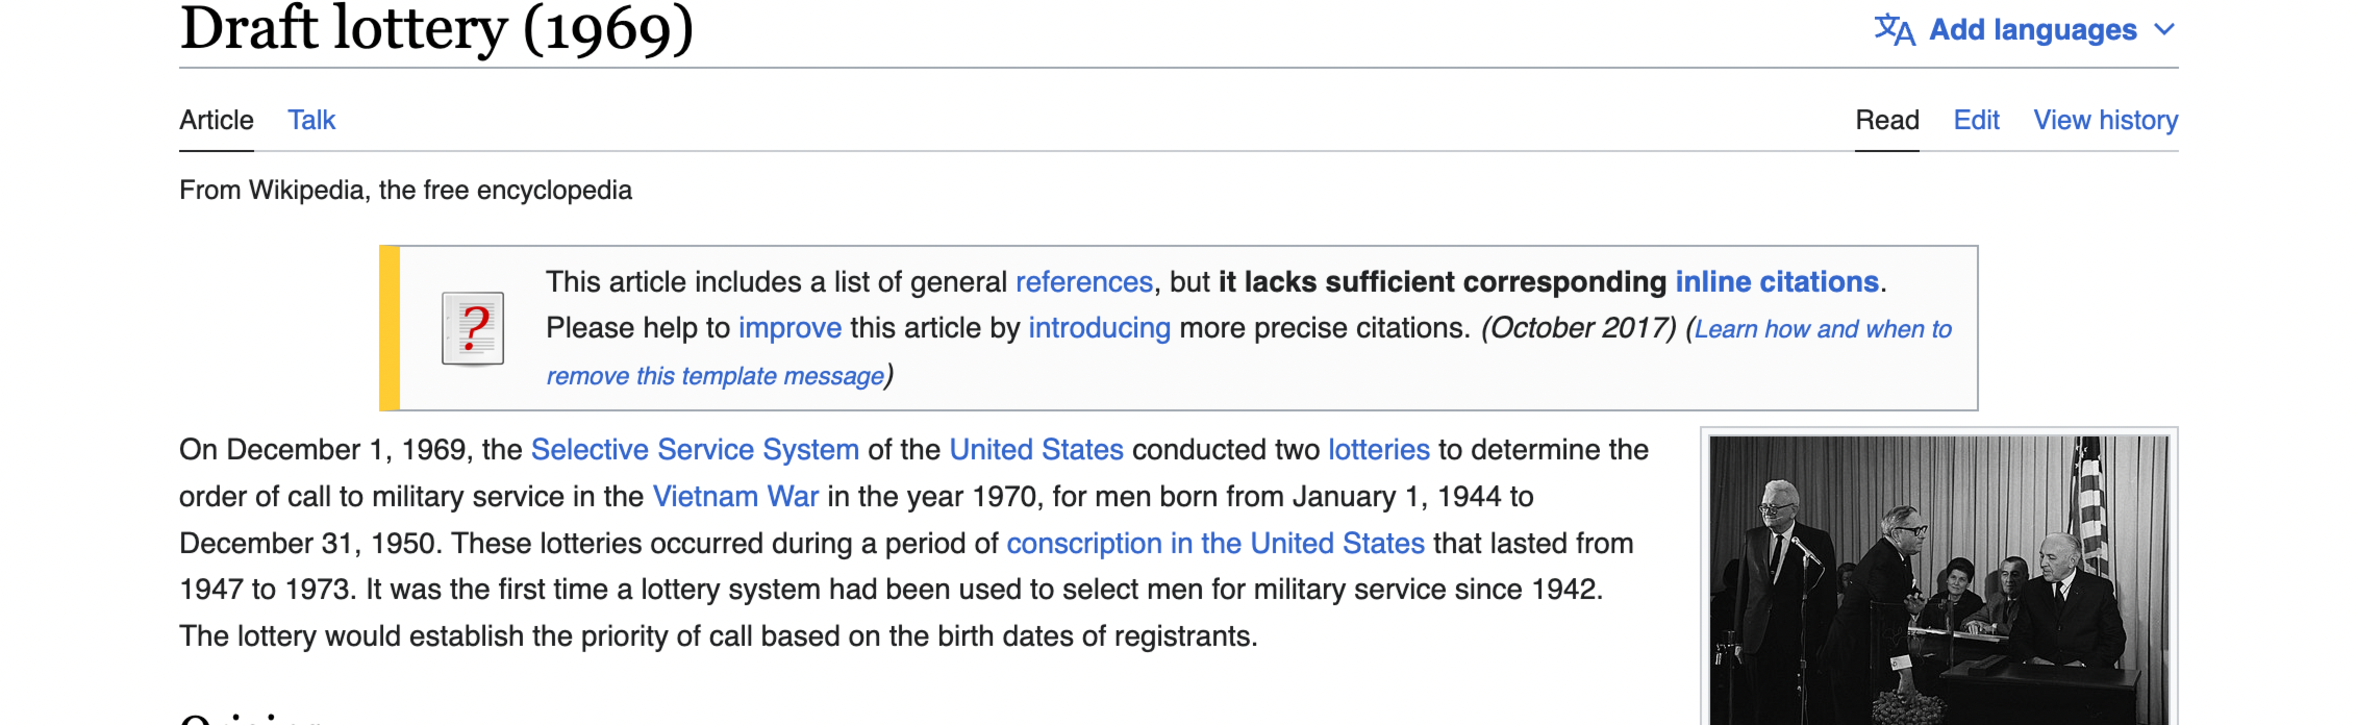
\includegraphics[width=1\textwidth]{assets/6/vietnam.pdf}
\end{frame}

\begin{frame}{Subpopulations}

\begin{itemize}
\item {\footnotesize{}Monotonicity implies that we can partition the population
into three groups:\medskip{}
}

\begin{enumerate}
\item \textbf{\footnotesize{}Never takers}{\footnotesize{} have $T_{i}(1)=T_{i}(0)=0$.
They don't take the treatment irrespective of the instrument.\medskip{}
}{\footnotesize\par}
\item \textbf{\footnotesize{}Always takers}{\footnotesize{} have $T_{i}(1)=T_{i}(0)=1$.
They take the treatment even if assigned $Z_{i}=0$.\medskip{}
}{\footnotesize\par}
\item \textbf{\footnotesize{}Compliers }{\footnotesize{}have $T_{i}(1)=1$
and $T_{i}(0)=0$ (equivalently, $T_{i}(1)>T(0)$). They take the
treatment if assigned $Z_{i}=1$, but not if assigned $Z_{i}=0$.
\medskip{}
}{\footnotesize\par}
\end{enumerate}
\item {\footnotesize{}Monotonicity rules out the existence of }\textbf{\footnotesize{}defiers}{\footnotesize{},
individuals with $T_{i}(1)=0$ but $T_{i}(0)=1$\medskip{}
}{\footnotesize\par}
\item {\footnotesize{}This terminology comes from randomized trials where
$Z_{i}$ is assignment to treatment and $T_{i}$ is receipt of treatment}{\footnotesize\par}
\end{itemize}
\end{frame}

\begin{frame}{The LATE Framework}

\begin{enumerate}
\item {\small{}Independence/Exclusion: $(Y_{i}(1),Y_{i}(0),T_{i}(1),T_{i}(0))\bot Z_{i}$\medskip{}
}{\small\par}
\item {\small{}First stage: $Pr\left[T_{i}=1|Z_{i}=1\right]>Pr\left[T_{i}=1|Z_{i}=0\right]$\medskip{}
}{\small\par}
\item {\small{}Monotonicity: $T_{i}(1)\geq T_{i}(0)\ \forall i$\medskip{}
}{\small\par}
\end{enumerate}
\begin{itemize}
\item {\small{}These three (really, 4) assumptions constitute the Local
Average Treatment Effect (LATE) framework (Imbens and Angrist 1994;
Angrist, Imbens and Rubin 1996)}{\small\par}
\end{itemize}
\end{frame}

\begin{frame}{The LATE Theorem}

\begin{itemize}
\item {\footnotesize{}In the LATE framework, IV estimates can be interpreted
as average causal effects for compliers, known as }\textbf{\footnotesize{}Local
Average Treatment Effects:}{\footnotesize\par}
\end{itemize}
\begin{center}
{\footnotesize{}$\dfrac{E\left[Y_{i}|Z_{i}=1\right]-E\left[Y_{i}|Z_{i}=0\right]}{E\left[T_{i}|Z_{i}=1\right]-E\left[T_{i}|Z_{i}=0\right]}=E\left[Y_{i}(1)-Y_{i}(0)|T_{i}(1)>T_{i}(0)\right]$}{\footnotesize\par}
\par\end{center}

\begin{center}
{\footnotesize{}$\equiv LATE$.}{\footnotesize\par}
\par\end{center}
\begin{itemize}
\item {\footnotesize{}The left-hand side is the IV (Wald) estimand\medskip{}
}{\footnotesize\par}
\item {\footnotesize{}The right-hand side is the average effect of treatment
for compliers, individuals who respond to the instrument by changing
treatment status\medskip{}
}{\footnotesize\par}
\item {\footnotesize{}This effect is ``local'' in the sense that it is
specific to the instrument used. Different instruments may yield different
LATEs!}{\footnotesize\par}
\end{itemize}
\end{frame}

\begin{frame}{The LATE Theorem: Proof}

\begin{itemize}
\item {\scriptsize{}The numerator of the Wald estimand, the reduced form,
is}{\scriptsize\par}
\end{itemize}
\begin{center}
{\scriptsize{}$E\left[Y_{i}|Z_{i}=1\right]-E\left[Y_{i}|Z_{i}=0\right]=E\left[Y_{i}(T_{i}(1))|Z_{i}=1\right]-E\left[Y_{i}(T_{i}(0))|Z_{i}=0\right]$}{\scriptsize\par}
\par\end{center}

\begin{center}
{\scriptsize{}$=E\left[Y_{i}(T_{i}(1))-Y_{i}(T_{i}(0))\right]$}{\scriptsize\par}
\par\end{center}

\begin{center}
{\scriptsize{}$=E\left[Y_{i}(T_{i}(1))-Y_{i}(T_{i}(0))|T_{i}(1)\neq T_{i}(0)\right]Pr\left[T_{i}(1)\neq T_{i}(0)\right]$}{\scriptsize\par}
\par\end{center}

\begin{center}
{\scriptsize{}$=E\left[Y_{i}(1)-Y_{i}(0)|T_{i}(1)>T_{i}(0)\right]Pr\left[T_{i}(1)>T_{i}(0)\right]$}{\scriptsize\par}
\par\end{center}

\end{frame}

\begin{frame}{The LATE Theorem: Proof}

\begin{itemize}
\item {\scriptsize{}The denominator of the Wald estimand, the first stage,
is}{\scriptsize\par}
\end{itemize}
\begin{center}
{\scriptsize{}$E\left[T_{i}|Z_{i}=1\right]-E\left[T_{i}|Z_{i}=0\right]=E\left[T_{i}(1)|Z_{i}=1\right]-E\left[T_{i}(0)|Z_{i}=0\right]$}{\scriptsize\par}
\par\end{center}

\begin{center}
{\scriptsize{}$=E\left[T_{i}(1)-T_{i}(0)\right]$}{\scriptsize\par}
\par\end{center}

\begin{center}
{\scriptsize{}$=Pr\left[T_{i}(1)>T_{i}(0)\right]$}{\scriptsize\par}
\par\end{center}

\end{frame}

\begin{frame}{The LATE Theorem: Proof}

\begin{itemize}
\item {\small{}Then the Wald estimand is}{\small\par}
\end{itemize}
\begin{center}
{\small{}$\dfrac{E\left[Y_{i}|Z_{i}=1\right]-E\left[Y_{i}|Z_{i}=0\right]}{E\left[T_{i}|Z_{i}=1\right]-E\left[T_{i}|Z_{i}=0\right]}=\dfrac{E\left[Y_{i}(1)-Y_{i}(0)|T_{i}(1)>T_{i}(0)\right]Pr\left[T_{i}(1)>T_{i}(0)\right]}{Pr\left[T_{i}(1)>T_{i}(0)\right]}$}{\small\par}
\par\end{center}

\begin{center}
{\small{}$=E\left[Y_{i}(1)-Y_{i}(0)|T_{i}(1)>T_{i}(0)\right]$.}{\small\par}
\par\end{center}

\end{frame}

\begin{frame}{The LATE Theorem: Discussion}

\begin{itemize}
\item {\small{}The LATE model is nonparametric: The LATE theorem applies
if $Y_{i}$ is binary, continuous, count, or any other distribution\medskip{}
}{\small\par}
\item {\small{}The LATE theorem provides useful guidance for interpreting
IV estimates and thinking about external validity\medskip{}
}{\small\par}
\item {\small{}Who are the compliers for the AK quarter of birth instrument?}{\small\par}
\end{itemize}
\end{frame}
\setbeamercolor{background canvas}{bg=} 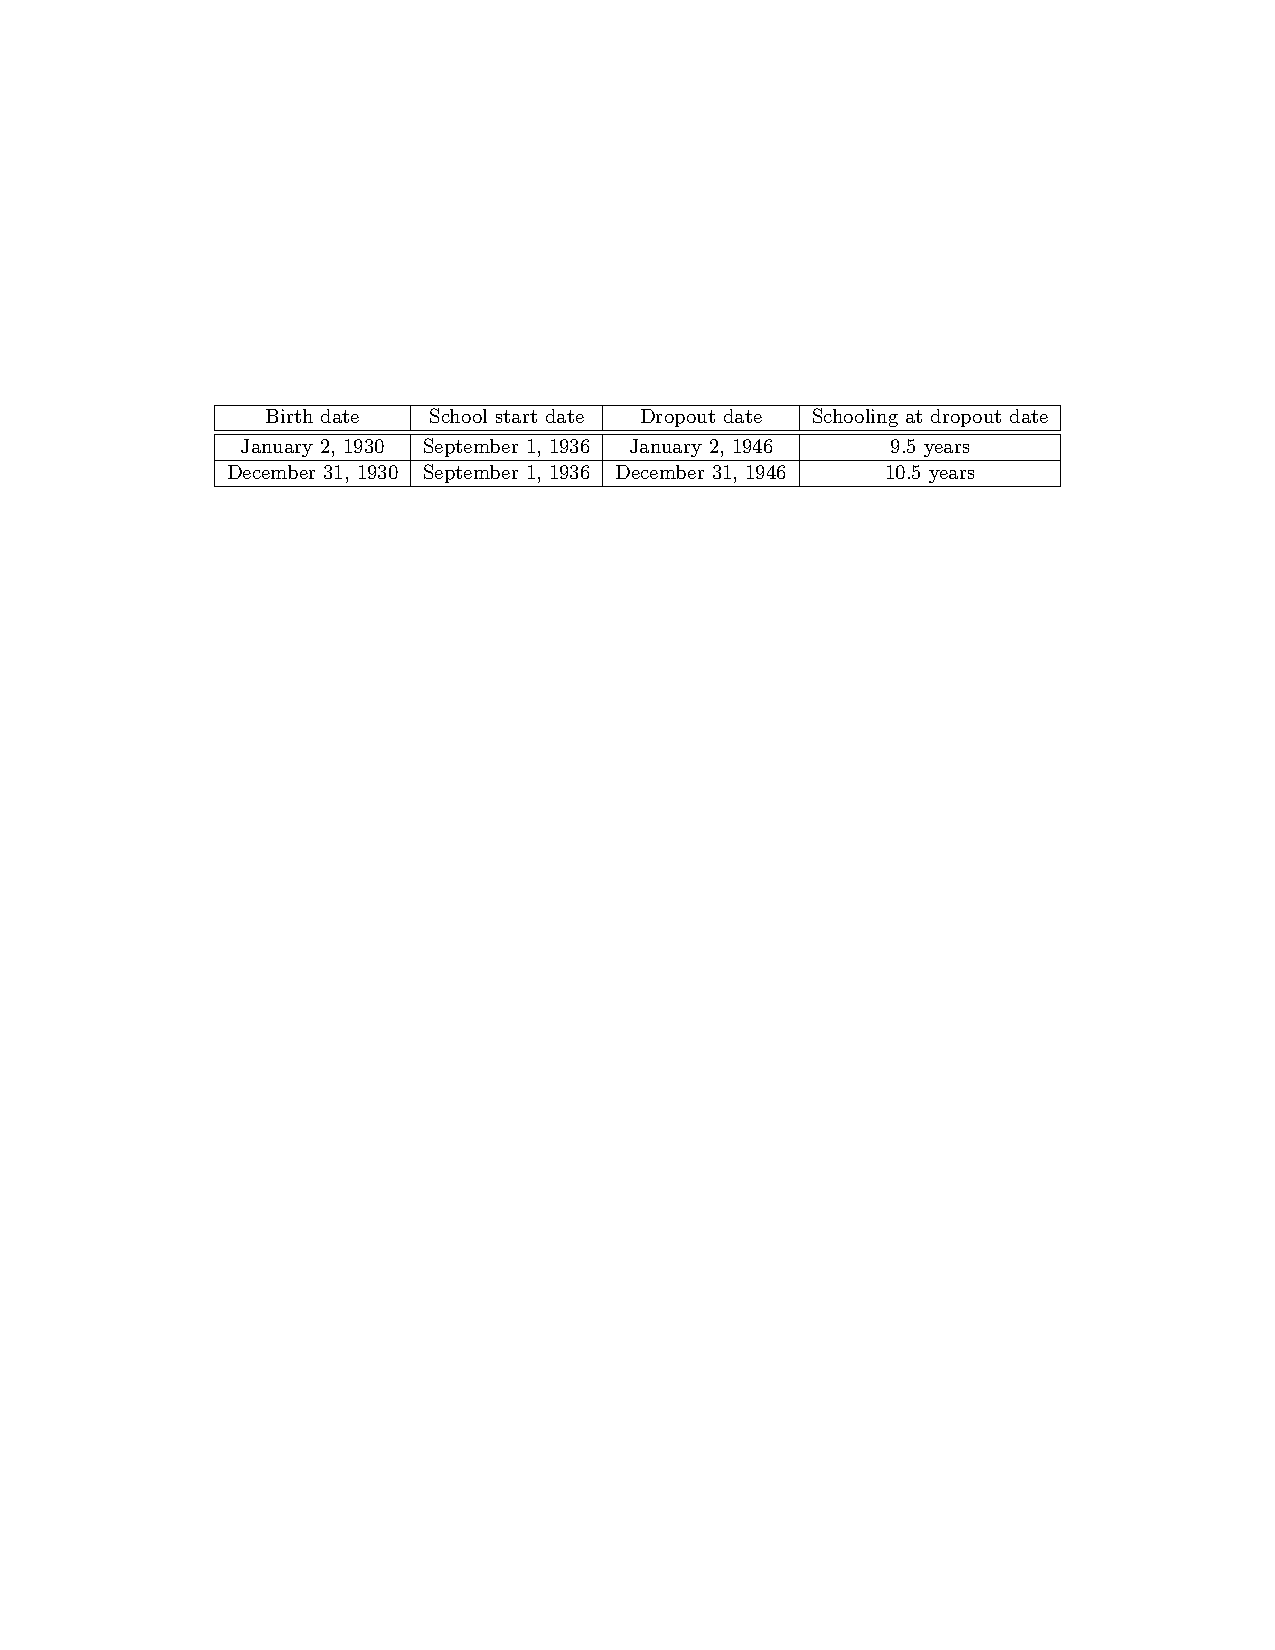
\includepdf{assets/6/qob_chart.pdf}
\setbeamercolor{background canvas}{bg=} 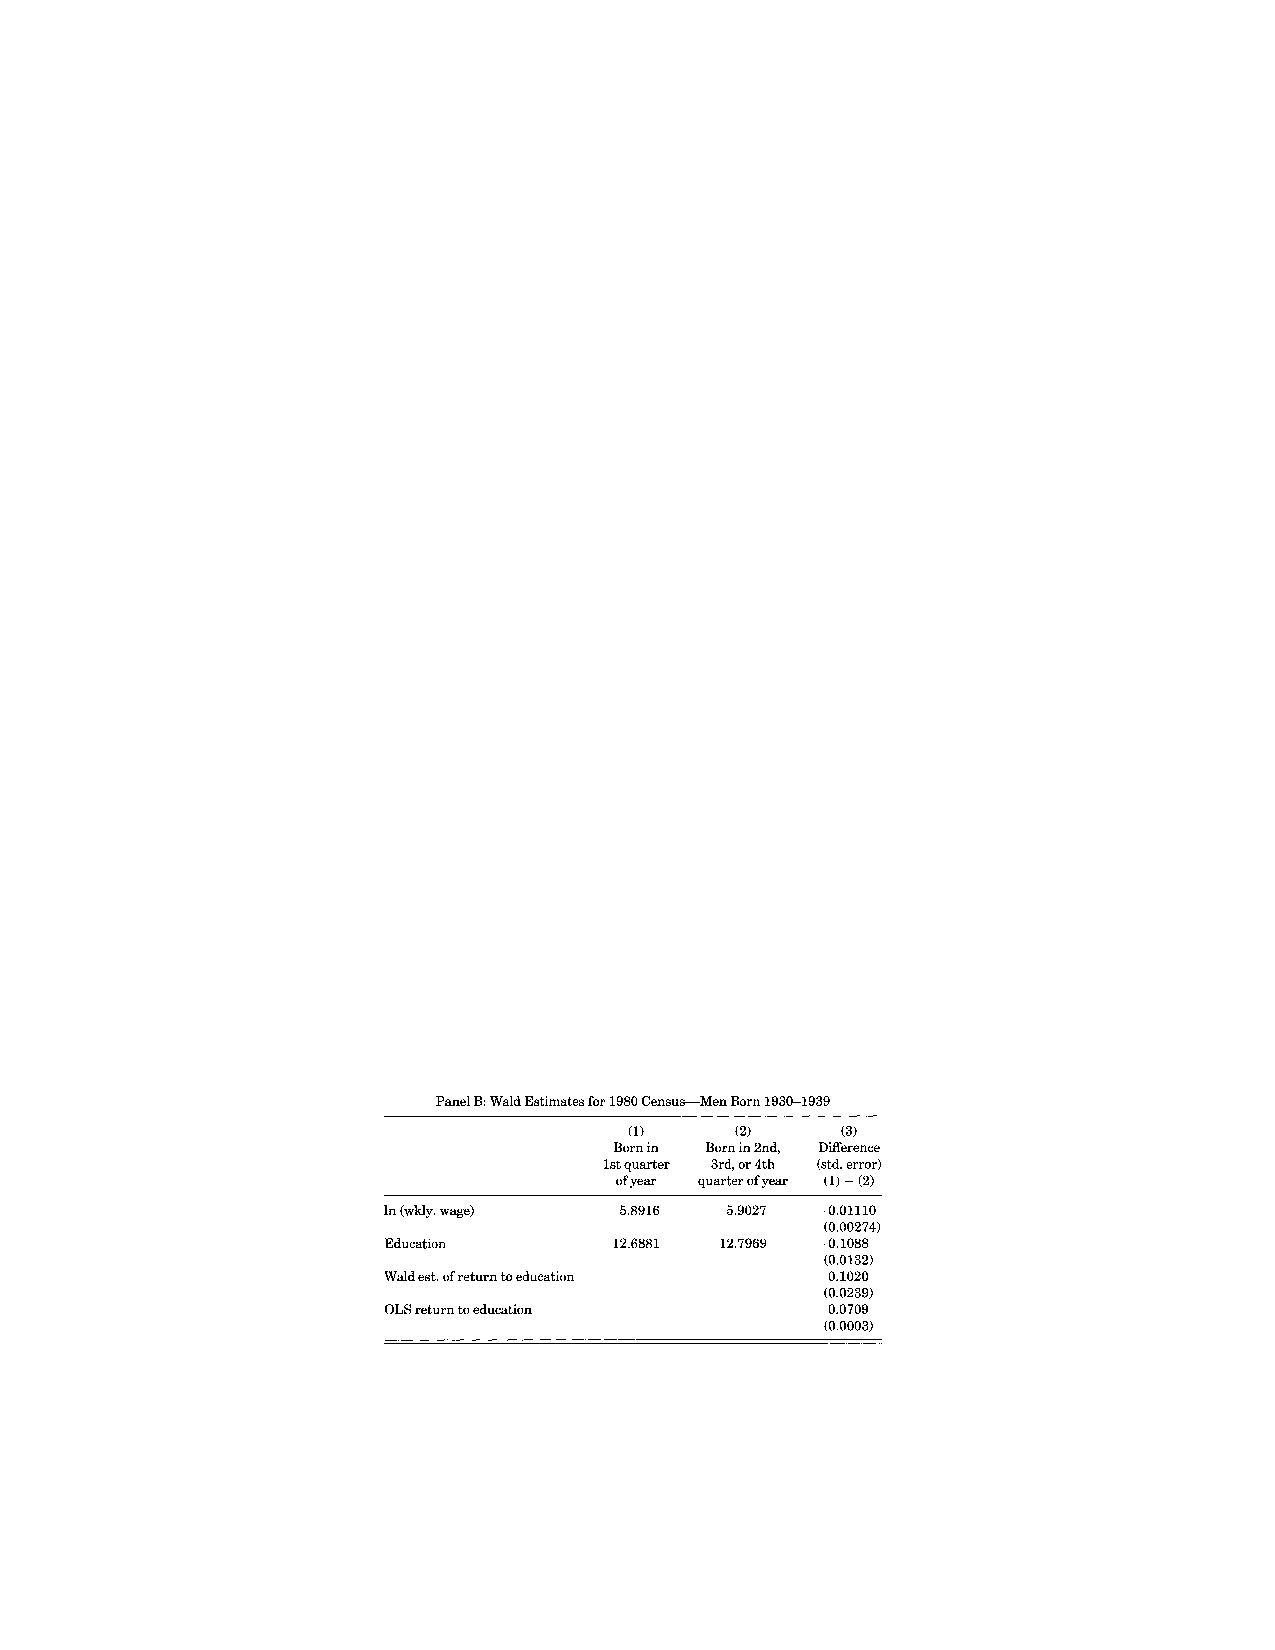
\includepdf{assets/6/angrist_krueger_1991_t3.pdf}

\begin{frame}{QOB Compliers}

\begin{itemize}
\item {\small{}The QOB compliers are individuals who drop out as soon as
possible, and are required to stay longer when their birthdays fall
late in the year\medskip{}
}{\small\par}
\item {\small{}Perhaps returns to schooling are higher for these individuals,
e.g. because returns are higher at low levels of schooling. Can this
explain $IV\geq OLS$?}{\small\par}
\end{itemize}
\end{frame}



\begin{frame}{LATE and Other Treatment Effects }

\begin{itemize}
\item {\footnotesize{}We can now add LATE to our catalogue of treatment
effects:\medskip{}
}

\begin{itemize}
\item {\footnotesize{}Average Treatment Effect:}{\footnotesize\par}
\end{itemize}
\begin{center}
{\footnotesize{}$ATE=E\left[Y_{i}(1)-Y_{i}(0)\right]$}{\footnotesize\par}
\par\end{center}
\begin{itemize}
\item {\footnotesize{}Effect of Treatment on the Treated: }{\footnotesize\par}
\end{itemize}
\begin{center}
{\footnotesize{}$TOT=E\left[Y_{i}(1)-Y_{i}(0)|T_{i}=1\right]$}{\footnotesize\par}
\par\end{center}
\begin{itemize}
\item {\footnotesize{}Effect of Treatment on the Non-Treated: }{\footnotesize\par}
\end{itemize}
\begin{center}
{\footnotesize{}$TNT=E\left[Y_{i}(1)-Y_{i}(0)|T_{i}=0\right]$}{\footnotesize\par}
\par\end{center}
\begin{itemize}
\item {\footnotesize{}Local Average Treatment Effect:}{\footnotesize\par}
\end{itemize}
\begin{center}
{\footnotesize{}$LATE=E\left[Y_{i}(1)-Y_{i}(0)|T_{i}(1)>T_{i}(0)\right]$\medskip{}
}{\footnotesize\par}
\par\end{center}
\item {\footnotesize{}How is LATE related to these other more general parameters?}{\footnotesize\par}
\end{itemize}
\end{frame}

\begin{frame}{The Bloom Scenario }

\begin{itemize}
\item {\footnotesize{}The $T_{i}=1$ population includes\medskip{}
}

\begin{itemize}
\item {\footnotesize{}Compliers with $Z_{i}=1$\medskip{}
}{\footnotesize\par}
\item {\footnotesize{}Always takers\medskip{}
}{\footnotesize\par}
\end{itemize}
\item {\footnotesize{}IV estimates do not capture effects for always takers
so in general $LATE\neq TOT$\medskip{}
}{\footnotesize\par}
\item {\footnotesize{}Suppose there is one-sided non-compliance, so that
$Z_{i}=0\implies T_{i}=0$\medskip{}
}{\footnotesize\par}
\item {\footnotesize{}Example: A medical trial where researchers can prevent
the control group from accessing the treatment but cannot force the
treatment group to take it\medskip{}
}{\footnotesize\par}
\item {\footnotesize{}In this case there are no always takers, so $LATE=TOT$\medskip{}
}{\footnotesize\par}
\item {\footnotesize{}This is the ``Bloom scenario'', after Bloom (1984)}{\footnotesize\par}
\end{itemize}
\end{frame}

\begin{frame}{LATE Example: MDVE }

\begin{itemize}
\item {\footnotesize{}LATE is useful for thinking about randomized experiments
where forcing compliance is either impossible or unethical\medskip{}
}{\footnotesize\par}
\item {\footnotesize{}Example: the Minneapolis Domestic Violence Experiment
(MDVE)\medskip{}
}{\footnotesize\par}
\item {\footnotesize{}The MDVE was an effort to determine the best response
to domestic violence calls\medskip{}
}{\footnotesize\par}
\item {\footnotesize{}Police responding to domestic violence calls can follow
two main strategies:\medskip{}
}

\begin{itemize}
\item {\footnotesize{}Arrest the offender (harsh)\medskip{}
}{\footnotesize\par}
\item {\footnotesize{}Warning/referal to counseling (``coddling'')\medskip{}
}{\footnotesize\par}
\end{itemize}
\item {\footnotesize{}Which of these two approaches leads to less domestic
violence in the future?}{\footnotesize\par}
\end{itemize}
\end{frame}

\begin{frame}{LATE Example: MDVE }

\begin{itemize}
\item {\small{}In the MDVE, police were given randomly-order color-coded
charge sheets, where colors indicated suggested strategy (arrest or
coddle)\medskip{}
}{\small\par}
\item {\small{}Enforcing compliance was unethical: some offenders are extremely
violent and may inflict injury if not immediately arrested\medskip{}
}{\small\par}
\item {\small{}Police were free to ignore suggestions if they deemed it
necessary\medskip{}
}{\small\par}
\item {\small{}Original literature on MDVE looked only at the reduced form
effect of assignment to arrest (``intent to treat'', ITT), but this
is a perfect IV scenario\medskip{}
}{\small\par}
\item {\small{}Very plausible that suggested arrest would weakly increase
the probability of arrest in all cases}{\small\par}
\end{itemize}
\end{frame}

\begin{frame}{LATE Example: MDVE }

\begin{itemize}
\item {\small{}Treatment $T_{i}$, is arrest\medskip{}
}{\small\par}
\item {\small{}Instrument $Z_{i}$ is assignment to arrest\medskip{}
}{\small\par}
\item {\small{}Outcome $Y_{i}$ is indicator for future offense\medskip{}
}{\small\par}
\item {\small{}In practice the police arrested everyone assigned to be arrest,
and also arrested some offenders assigned to coddling\medskip{}
}{\small\par}
\item {\small{}How should we interpret IV estimates from the MDVE?}{\small\par}
\end{itemize}
\end{frame}

\begin{frame}{LATE Example: MDVE }

\begin{itemize}
\item {\small{}In the MDVE, $Z_{i}=1\implies T_{i}=1$\medskip{}
}{\small\par}
\item {\small{}There are no never takers since everyone assigned to treatment
is treated\medskip{}
}{\small\par}
\item {\small{}As a result everyone who is coddled is a complier\medskip{}
}{\small\par}
\item {\small{}This is the flip of the Bloom scenario: $LATE=TNT$\medskip{}
}{\small\par}
\item {\small{}The MDVE identifies the effect of arrest on the coddled}{\small\par}
\end{itemize}
\end{frame}
\subsection{Characterizing Compliers}
\begin{frame}{Characterizing Compliers }

\begin{itemize}
\item {\small{}To interpret any IV estimate, it's useful to ask: Who are
the compliers?\medskip{}
}{\small\par}
\item {\small{}It turns out that we can learn a lot about the compliers\medskip{}
}{\small\par}
\item {\small{}Consider the subpopulations captured in each combination
of $T_{i}$ and $Z_{i}$:}{\small\par}
\end{itemize}
\begin{center}
{\small{}}%
\begin{tabular}{|c|c|c|}
\hline 
 & {\small{}$T_{i}=1$} & {\small{}$T_{i}=0$}\tabularnewline
\hline 
\hline 
{\small{}$Z_{i}=1$} & {\small{}Compliers and Always takers} & {\small{}Never takers}\tabularnewline
\hline 
{\small{}$Z_{i}=0$} & {\small{}Always takers} & {\small{}Compliers and Never takers}\tabularnewline
\hline 
\end{tabular}{\small\par}
\par\end{center}

\end{frame}

\begin{frame}{Characterizing Compliers }

\begin{center}
{\footnotesize{}}%
\begin{tabular}{|c|c|c|}
\hline 
 & {\footnotesize{}$T_{i}=1$} & {\footnotesize{}$T_{i}=0$}\tabularnewline
\hline 
\hline 
{\footnotesize{}$Z_{i}=1$} & {\footnotesize{}Compliers and Always takers} & {\footnotesize{}Never takers}\tabularnewline
\hline 
{\footnotesize{}$Z_{i}=0$} & {\footnotesize{}Always takers} & {\footnotesize{}Compliers and Never takers}\tabularnewline
\hline 
\end{tabular}{\footnotesize\par}
\par\end{center}
\begin{itemize}
\item {\footnotesize{}Always takers are directly observable in the $(Z_{i}=0,T_{i}=1)$
group\medskip{}
}{\footnotesize\par}
\item {\footnotesize{}Never takers are directly observable in the $(Z_{i}=1,T_{i}=0)$
group\medskip{}
}{\footnotesize\par}
\item {\footnotesize{}The groups with $T_{i}=Z_{i}$ are mixtures of ATs/compliers
and NTs/compliers\medskip{}
}{\footnotesize\par}
\item {\footnotesize{}But note that the mixing probabilities are identified,
since}{\footnotesize\par}
\end{itemize}
\begin{center}
{\footnotesize{}$\pi^{at}=Pr\left[T_{i}(1)=T_{i}(0)=1\right]=Pr\left[T_{i}=1|Z_{i}=0\right]$}{\footnotesize\par}
\par\end{center}

\begin{center}
{\footnotesize{}$\pi^{nt}=Pr\left[T_{i}(1)=T_{i}(0)=0\right]=Pr\left[T_{i}=0|Z_{i}=1\right]$}{\footnotesize\par}
\par\end{center}

\begin{center}
{\footnotesize{}$\pi^{c}=Pr\left[T_{i}(1)>T_{i}(0)\right]=Pr\left[T_{i}=1|Z_{i}=1\right]-Pr\left[T_{i}=1|Z_{i}=0\right]$}{\footnotesize\par}
\par\end{center}

\end{frame}

\begin{frame}{Characterizing Compliers }

\begin{itemize}
\item {\footnotesize{}For an observed covariate $X_{i}$ we have}{\footnotesize\par}
\end{itemize}
\begin{center}
{\footnotesize{}$E\left[X_{i}|T_{i}=Z=1\right]=\left(\tfrac{\pi^{c}}{\pi^{c}+\pi^{at}}\right)E\left[X_{i}|T_{i}(1)>T_{i}(0)\right]$}{\footnotesize\par}
\par\end{center}

\begin{center}
{\footnotesize{}$+\left(\tfrac{\pi^{at}}{\pi^{c}+\pi^{at}}\right)E\left[X_{i}|T_{i}(1)=T_{i}(0)=1\right]$}{\footnotesize\par}
\par\end{center}
\begin{itemize}
\item {\footnotesize{}The mean for the $T_{i}=Z_{i}=1$ group is a weighted
average of complier and always taker means, with known weights\medskip{}
}{\footnotesize\par}
\item {\footnotesize{}The always taker mean is identified since $E\left[X_{i}|T_{i}(1)=T_{i}(0)=1\right]=E\left[X_{i}|T_{i}=1,Z_{i}=0\right]$\medskip{}
}{\footnotesize\par}
\item {\footnotesize{}Then the complier mean is also identified:}{\footnotesize\par}
\end{itemize}
\begin{center}
{\footnotesize{}$E\left[X_{i}|T_{i}(1)>T_{i}(0)\right]=\left(\tfrac{\pi^{c}+\pi^{at}}{\pi^{c}}\right)E\left[X_{i}|T_{i}=Z_{i}=1\right]$}{\footnotesize\par}
\par\end{center}

\begin{center}
{\footnotesize{}$-\left(\tfrac{\pi^{at}}{\pi^{c}}\right)E\left[X_{i}|T_{i}=1,Z_{i}=0\right]$}{\footnotesize\par}
\par\end{center}

\end{frame}

\begin{frame}{Characterizing Compliers }

\begin{center}
{\footnotesize{}$E\left[X_{i}|T_{i}(1)>T_{i}(0)\right]=\left(\tfrac{\pi^{c}+\pi^{at}}{\pi^{c}}\right)E\left[X_{i}|T_{i}=Z_{i}=1\right]$}{\footnotesize\par}
\par\end{center}

\begin{center}
{\footnotesize{}$-\left(\tfrac{\pi^{at}}{\pi^{c}}\right)E\left[X_{i}|T_{i}=1,Z_{i}=0\right]$}{\footnotesize\par}
\par\end{center}
\begin{itemize}
\item {\footnotesize{}The complier mean of $X_{i}$ can be recovered by
removing the always taker mean from the complier/always taker mixer,
adjusting appropriately for relative probabilities\medskip{}
}{\footnotesize\par}
\item {\footnotesize{}This means we can learn the observed characteristics
of compliers as if they were observable in our data}{\footnotesize\par}
\end{itemize}
\end{frame}

\begin{frame}{Complier Mean Potential Outcomes}

\begin{itemize}
\item {\small{}We could have substituted the outcome $Y_{i}$ in place of
$X_{i}$ in this argument\medskip{}
}{\small\par}
\item {\small{}This implies that the marginal mean of $Y_{i}(1)$ for compliers,
$E\left[Y_{i}(1)|T_{i}(1)>T_{i}(0)\right]$, is also identified\medskip{}
}{\small\par}
\item {\small{}Likewise, $E\left[Y_{i}(0)|T_{i}(1)>T_{i}(0)\right]$ can
be obtained by removing the never taker mean outcome from the $Z_{i}=T_{i}=0$
mixture\medskip{}
}{\small\par}
\item {\small{}The }\emph{\small{}levels}{\small{} of complier mean potential
outcomes are therefore identified, not just the difference between
them}{\small\par}
\end{itemize}
\end{frame}

\begin{frame}{Computing Complier Characteristics}

\begin{itemize}
\item {\footnotesize{}Abadie (2002) provides a convenient method for computing
complier characteristics\medskip{}
}{\footnotesize\par}
\item {\footnotesize{}For any measureable function $g(X_{i},Y_{i})$: }{\footnotesize\par}
\end{itemize}
\begin{center}
{\scriptsize{}$\dfrac{E\left[g(X_{i},Y_{i})T_{i}|Z_{i}=1\right]-E\left[g(X_{i},Y_{i})T_{i}|Z_{i}=0\right]}{E\left[T_{i}|Z_{i}=1\right]-E\left[T_{i}|Z_{i}=0\right]}=E\left[g(X_{i,}Y_{i}(1))|T_{i}(1)>T_{i}(0)\right]$}{\scriptsize\par}
\par\end{center}

\begin{center}
{\scriptsize{}$\dfrac{E\left[g(X_{i},Y_{i})(1-T_{i})|Z_{i}=1\right]-E\left[g(X_{i},Y_{i})(1-T_{i})|Z_{i}=0\right]}{E\left[1-T_{i}|Z_{i}=1\right]-E\left[1-T_{i}|Z_{i}=0\right]}$}{\scriptsize\par}
\par\end{center}

\begin{center}
{\scriptsize{}$=E\left[g(X_{i,}Y_{i}(0))|T_{i}(1)>T_{i}(0)\right]$}{\scriptsize\par}
\par\end{center}

\end{frame}

\begin{frame}{Computing Complier Characteristics}

\begin{itemize}
\item {\small{}Abadie's result shows that in the IV system}{\small\par}
\end{itemize}
\begin{center}
{\small{}$g(X_{i},Y_{i})T_{i}=\alpha+\gamma T_{i}+u_{i}$}{\small\par}
\par\end{center}

\begin{center}
{\small{}$T_{i}=\lambda+\pi Z_{i}+\eta_{i}$,}{\small\par}
\par\end{center}
\begin{itemize}
\item {\small{}The IV coefficient $\gamma$ recovers the treated complier
mean of $g$:}{\small\par}
\end{itemize}
\begin{center}
{\small{}$\gamma=E\left[g(X_{i},Y_{i}(1))|T_{i}(1)>T_{i}(0)\right]$}{\small\par}
\par\end{center}
\begin{itemize}
\item {\small{}Substitute $(1-T_{i})$ for $T_{i}$ in both equations to
obtain the untreated complier mean}{\small\par}
\end{itemize}
\end{frame}

\begin{frame}{Computing Complier Characteristics}

\begin{itemize}
\item {\small{}Useful special cases:\medskip{}
}

\begin{itemize}
\item {\small{}$g(X_{i},Y_{i})=X_{i}$: Complier mean of $X_{i}$\medskip{}
}{\small\par}
\item {\small{}$g(X_{i},Y_{i})=Y_{i}$ : Marginal complier means of $Y_{i}(1)$
and $Y_{i}(0)$\medskip{}
}{\small\par}
\item {\small{}$g(X_{i},Y_{i})=1\left\{ Y_{i}\leq y\right\} $: Complier
CDFs of $Y_{i}(1)$ and $Y_{i}(0)$ evaluated at $y$\medskip{}
}{\small\par}
\end{itemize}
\item {\small{}This last result shows that the full marginal distributions
of $Y_{i}(1)$ and $Y_{i}(0)$ are identified for compliers}{\small\par}
\end{itemize}
\end{frame}
 \setbeamercolor{background canvas}{bg=}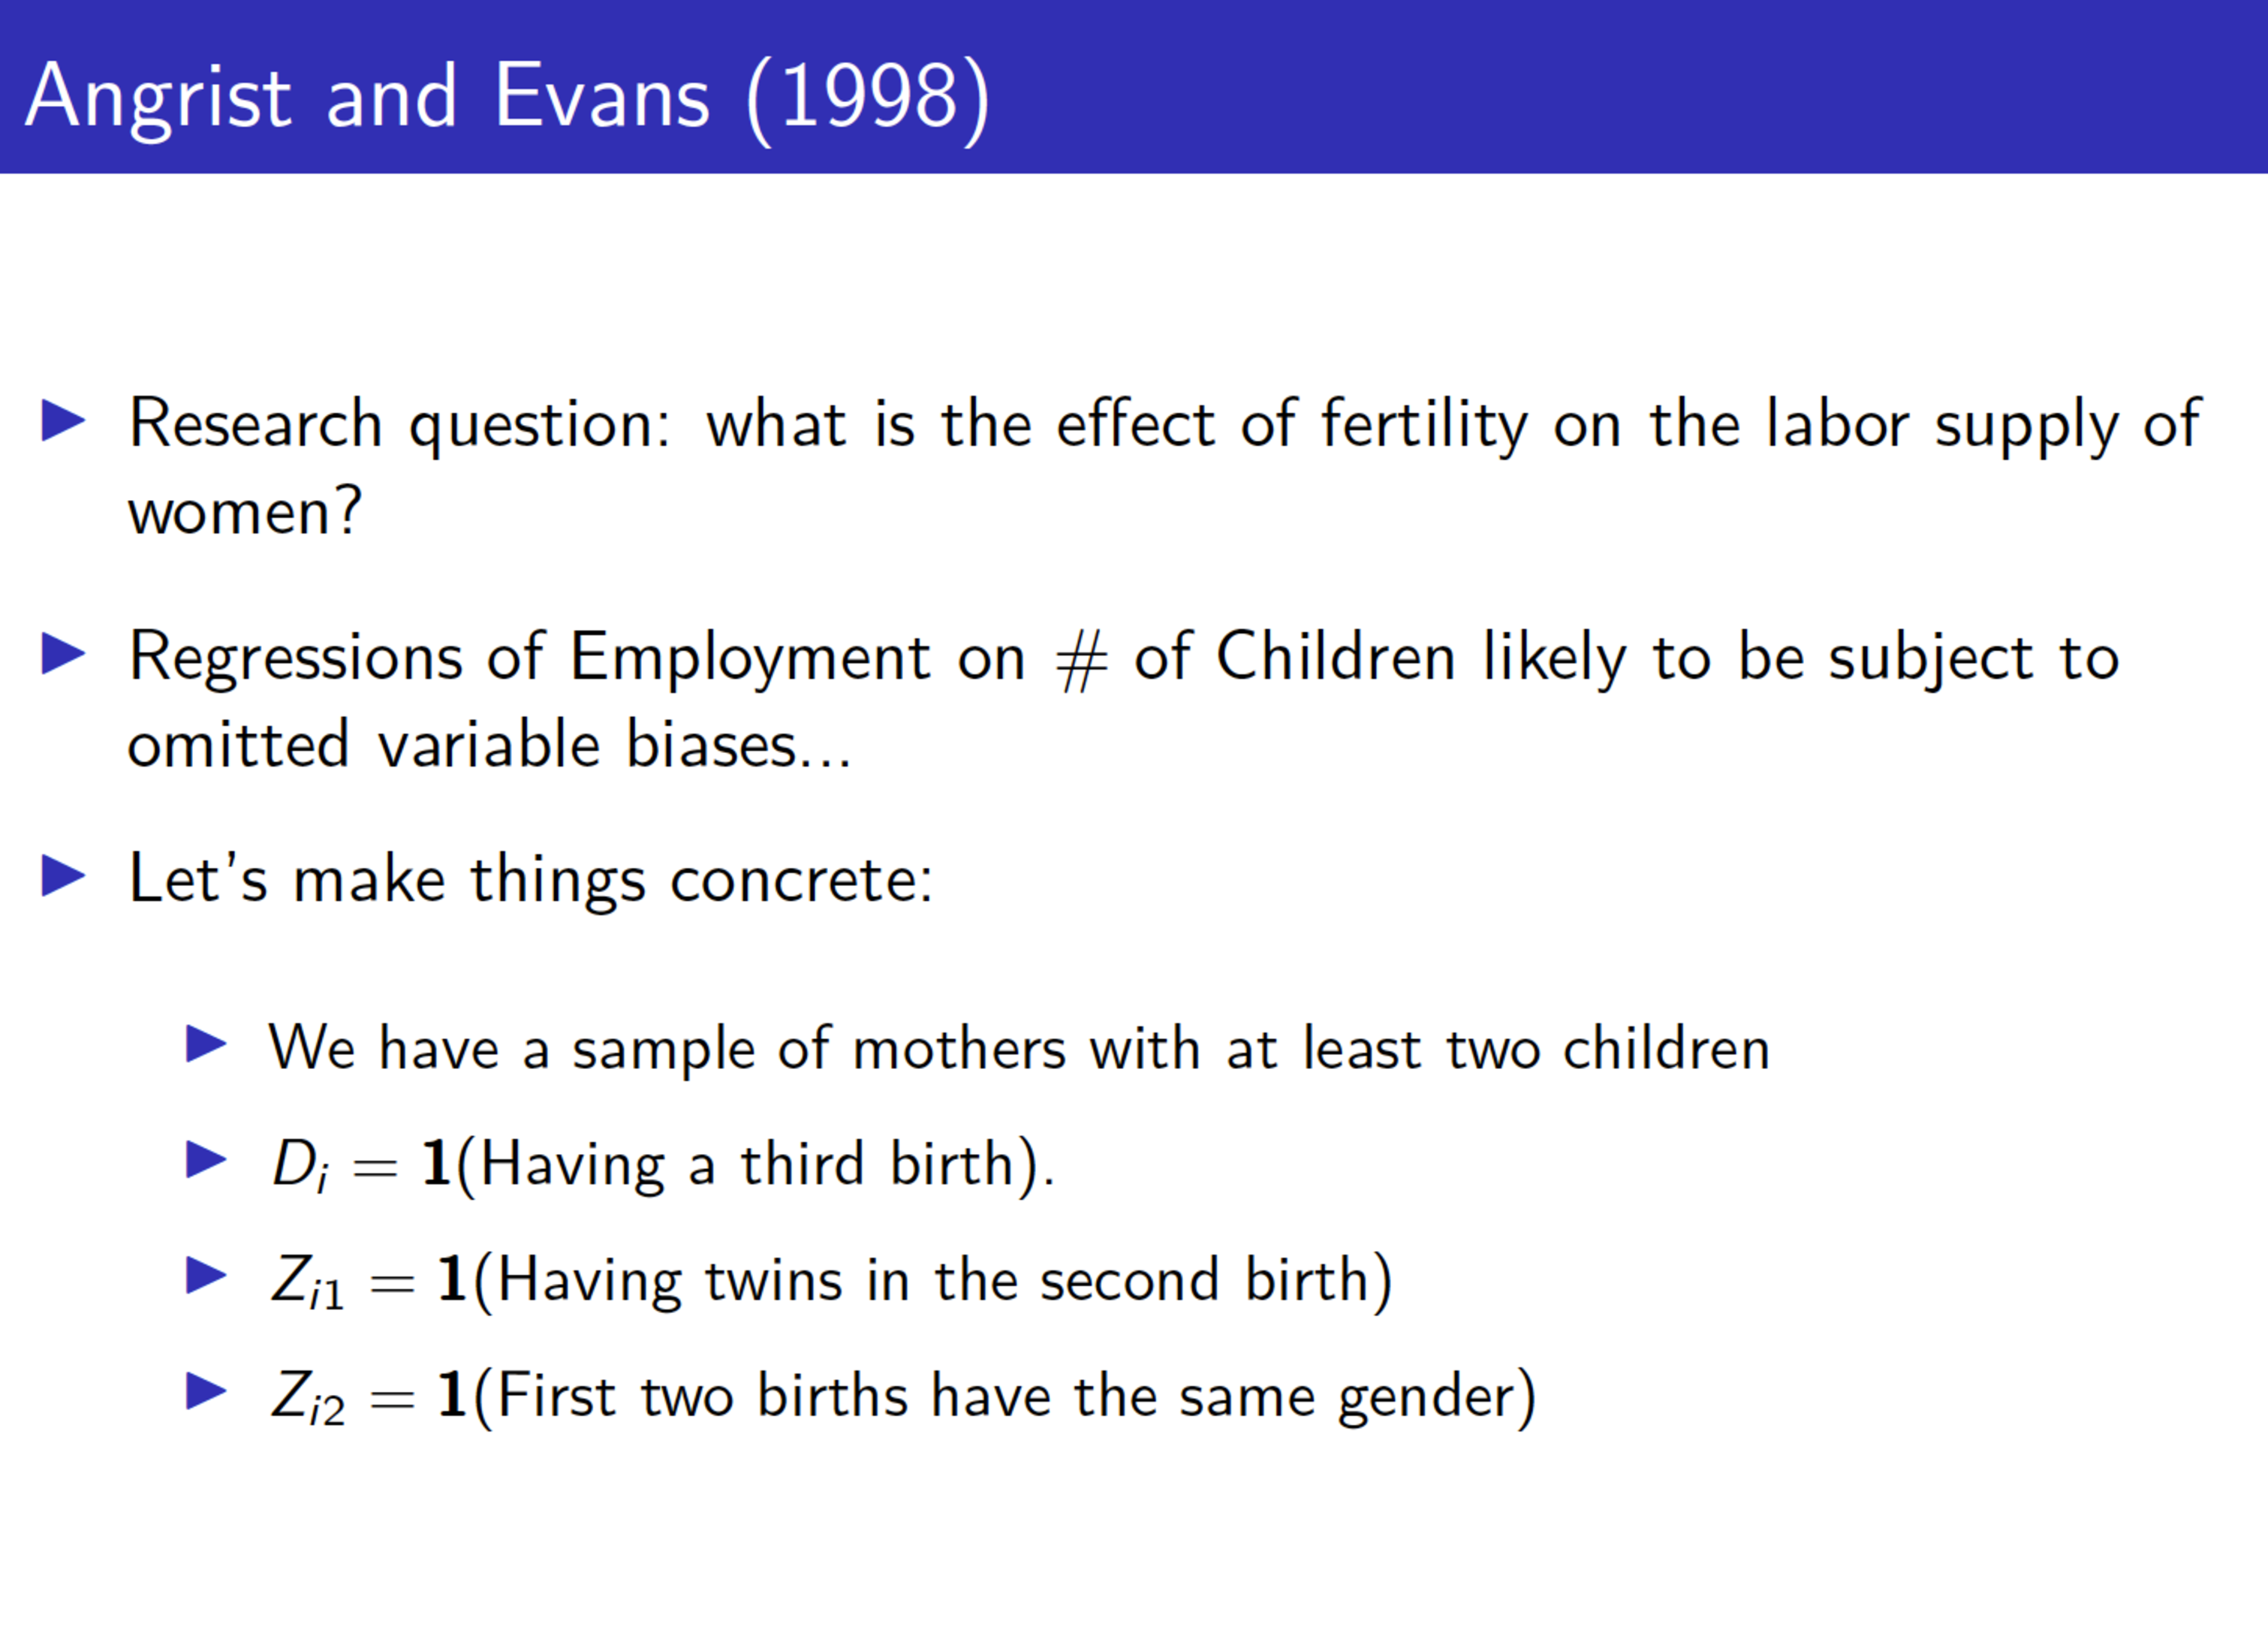
\includepdf{assets/6/exp1.pdf}
 \setbeamercolor{background canvas}{bg=}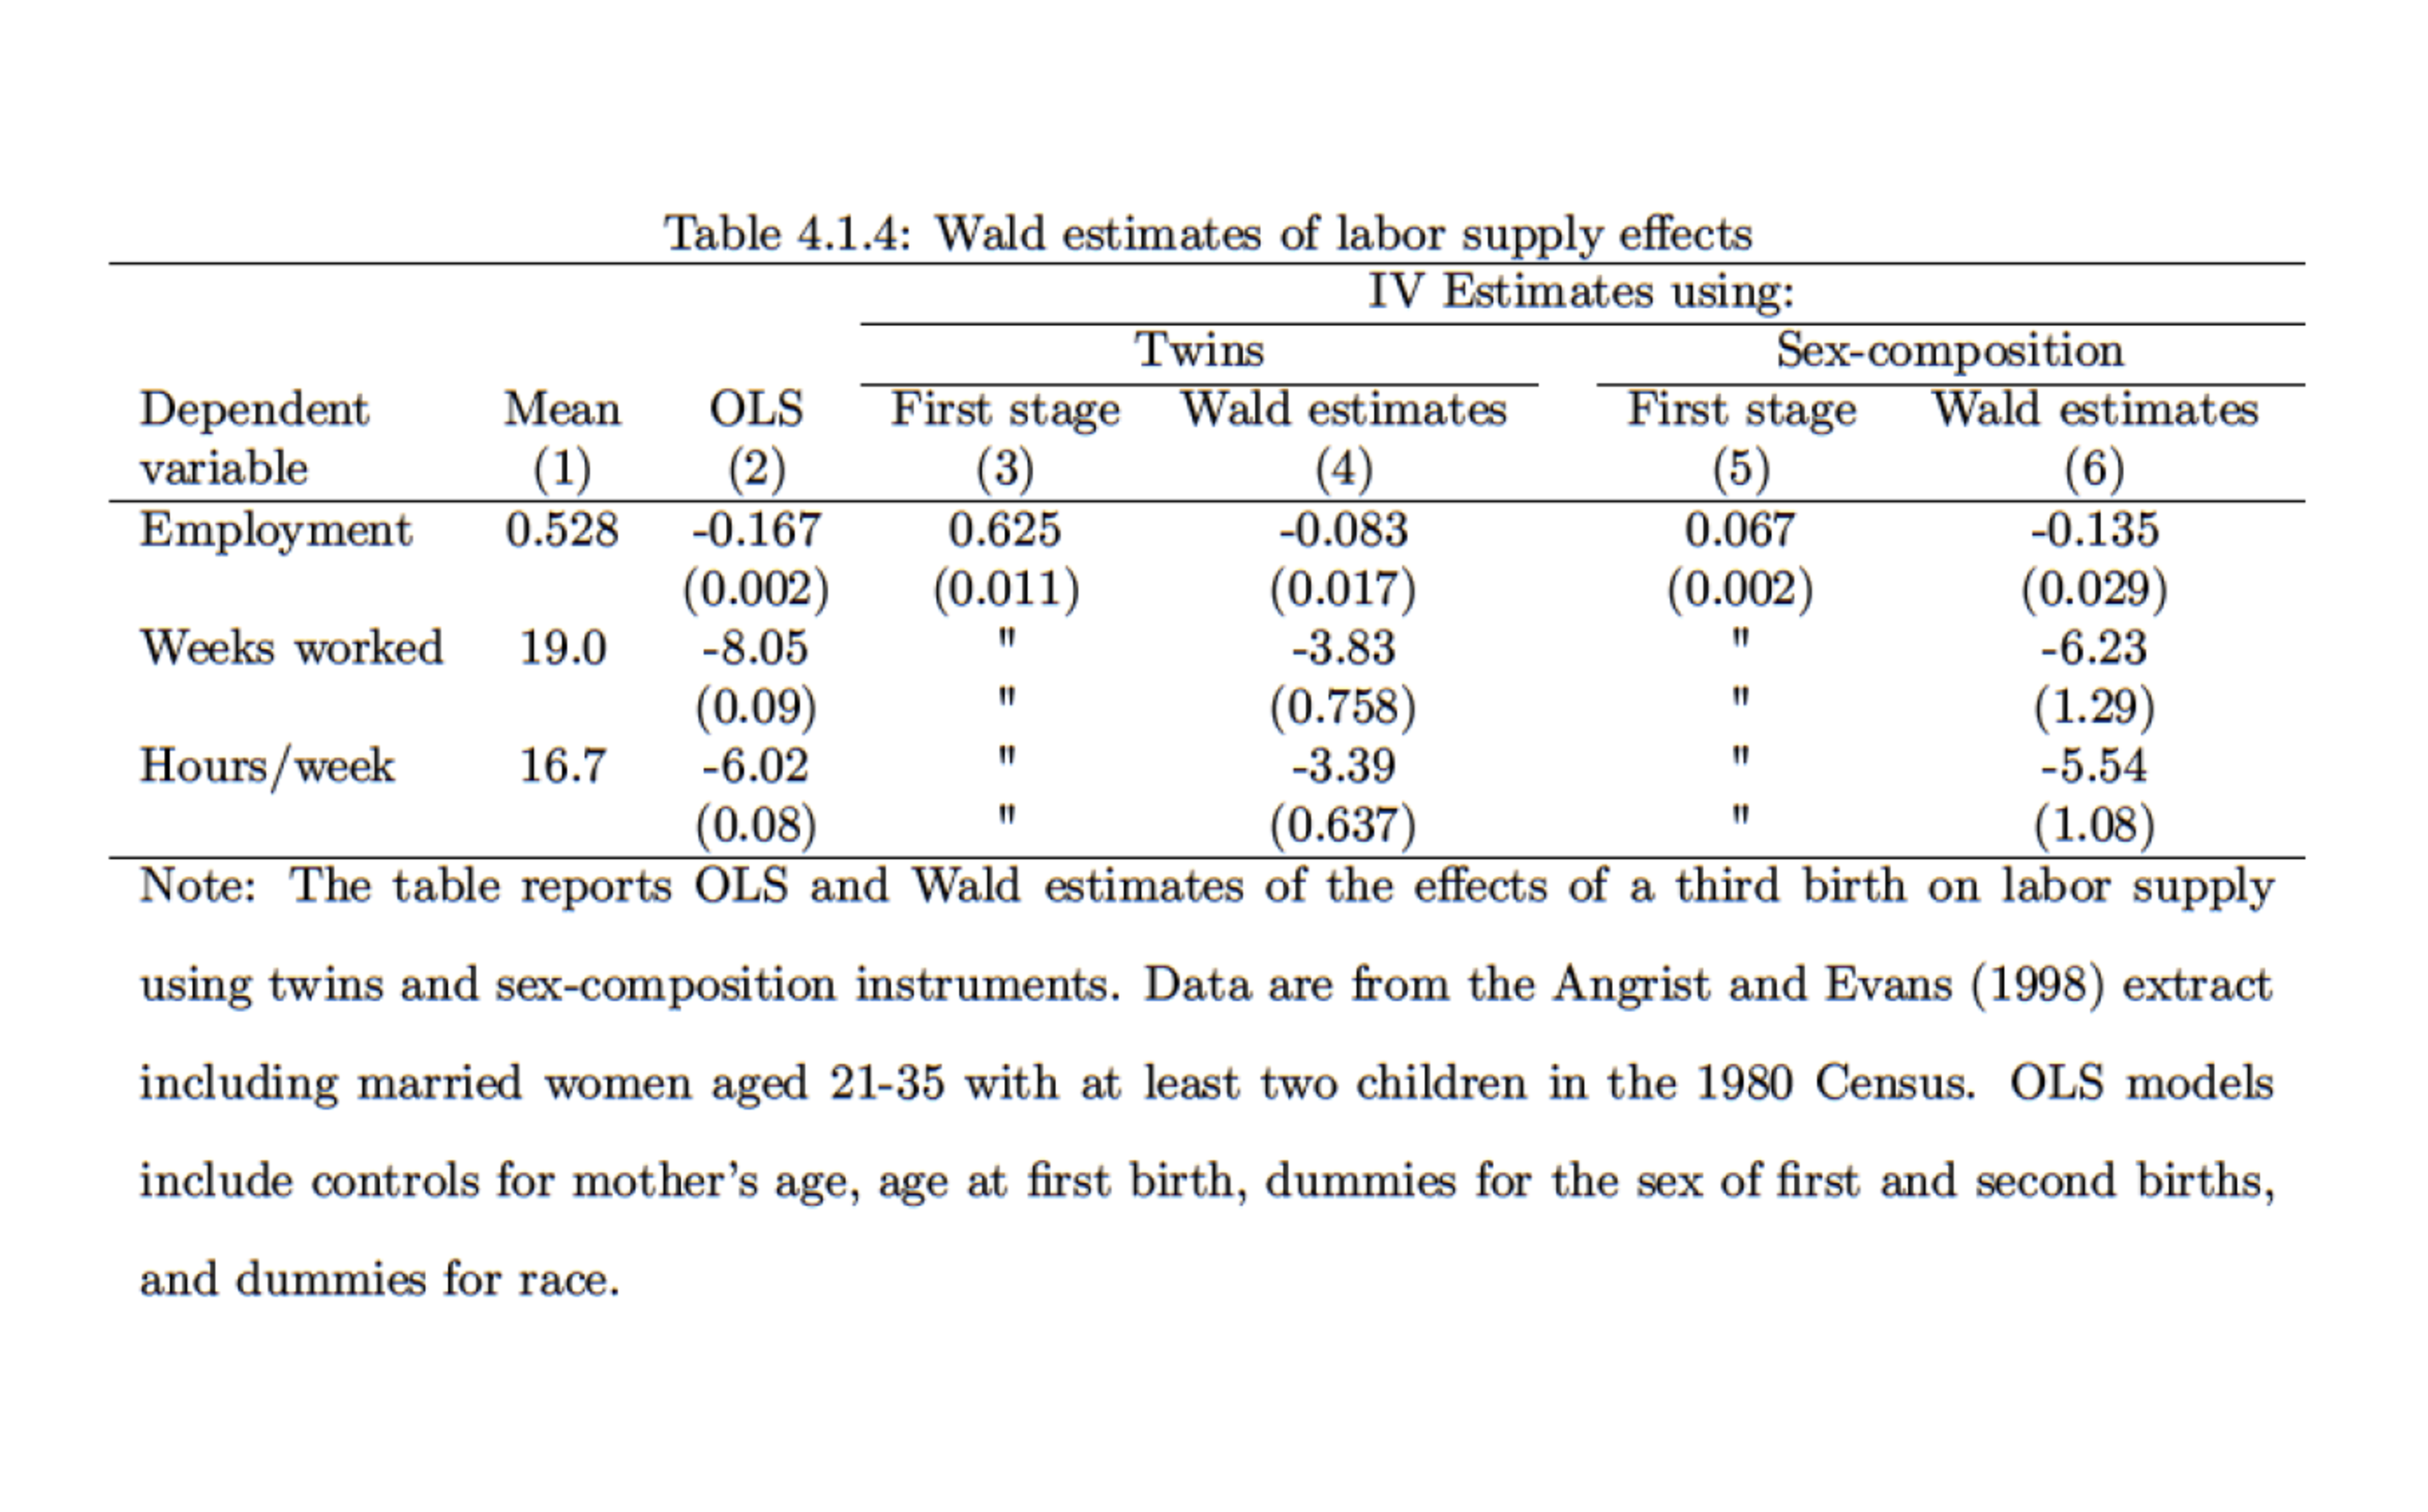
\includepdf{assets/6/exp2.pdf}
  \setbeamercolor{background canvas}{bg=}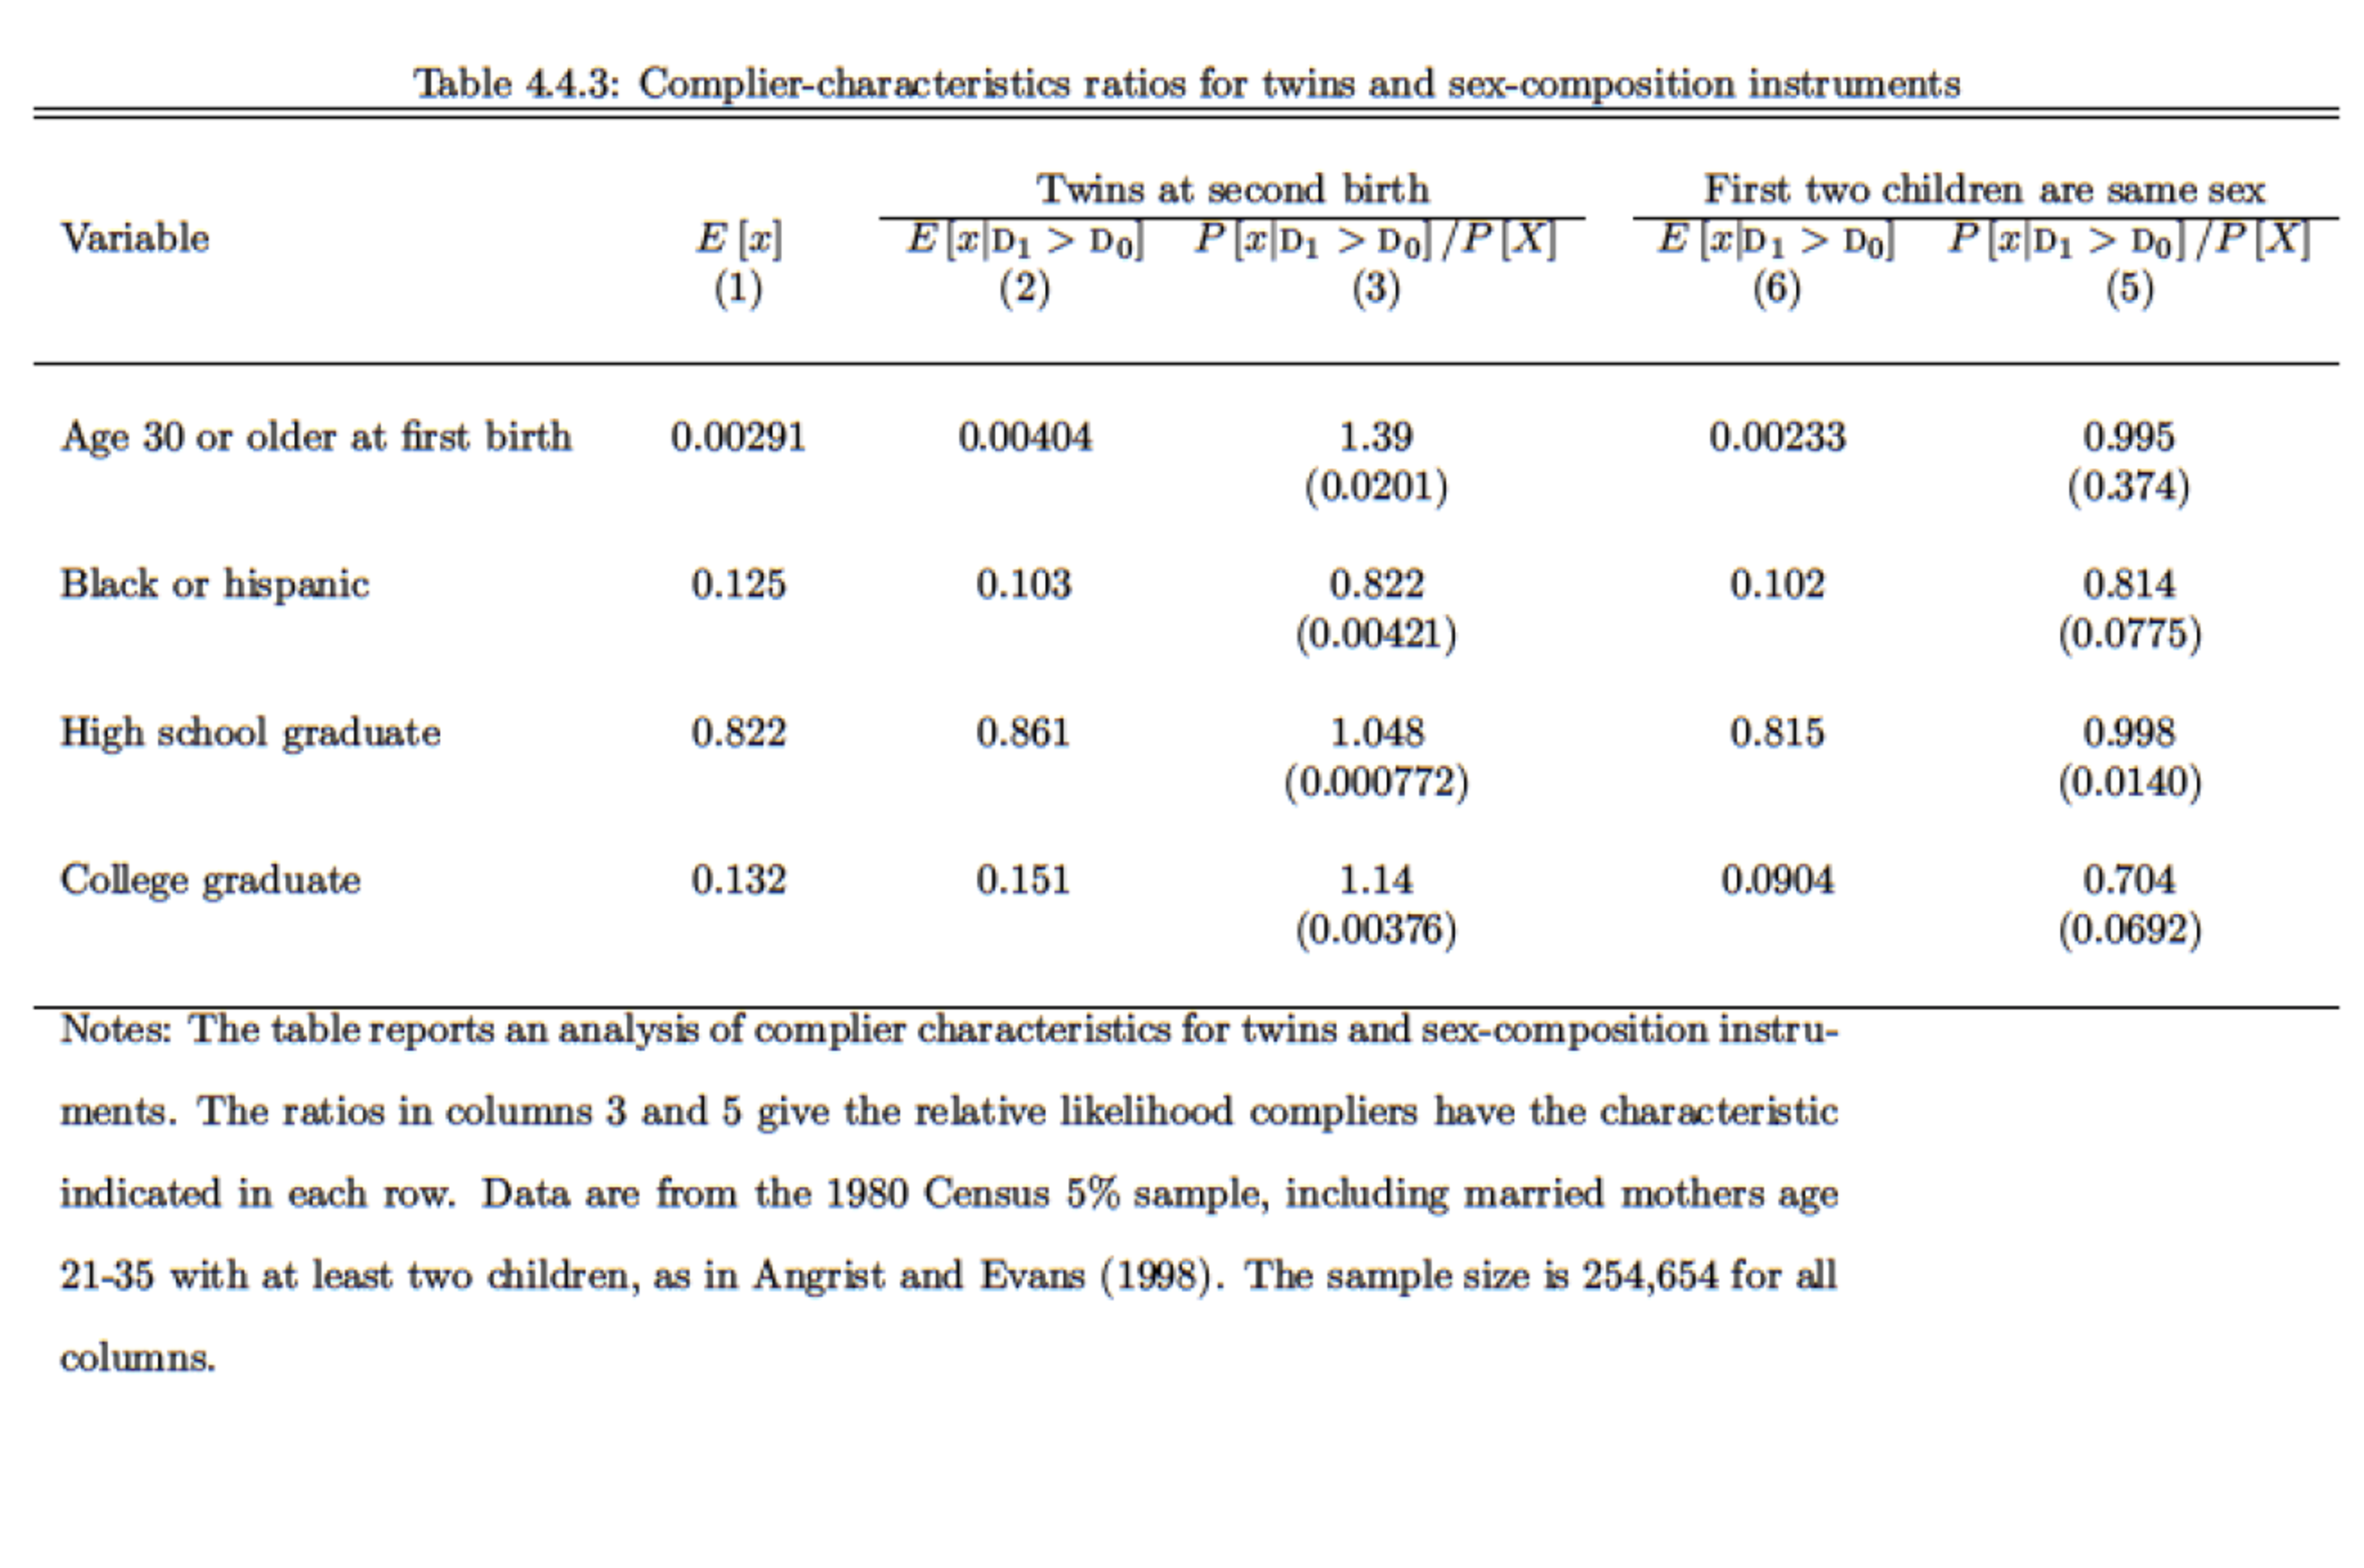
\includepdf{assets/6/exp3.pdf}



\begin{frame}{Back to Overid Tests }

\begin{itemize}
\item {\footnotesize{}Informed by our discussion of heterogeneous effects,
let's return to overid tests\medskip{}
}{\footnotesize\par}
\item {\footnotesize{}As discussed earlier, overid tests reject when different
instruments yield different parameter estimates\medskip{}
}{\footnotesize\par}
\item {\footnotesize{}In a constant effects model, this implies that at
least one must be invalid\medskip{}
}{\footnotesize\par}
\item {\footnotesize{}In a heterogeneous effect model, they may identify
different LATEs\medskip{}
}{\footnotesize\par}
\item {\footnotesize{}Can we distinguish between invalid instruments and
treatment effect heterogeneity?}{\footnotesize\par}
\end{itemize}
\end{frame}




\begin{frame}{Back to Overid Tests }

\begin{itemize}
\item {\footnotesize{}To fix ideas, return to a model with binary treatment
$T_{i}$, binary instrument $Z_{i}$, and covariates $X_{i}$. Saturated
2SLS model:}{\footnotesize\par}
\end{itemize}
\begin{center}
{\footnotesize{}$Y_{i}=X_{i}^{\prime}\alpha+\rho T_{i}+\varepsilon_{i}$}{\footnotesize\par}
\par\end{center}

\begin{center}
{\footnotesize{}$T_{i}=X_{i}^{\prime}\lambda+Z_{i}\cdot X_{i}^{\prime}\pi+\eta_{i}$}{\footnotesize\par}
\par\end{center}
\begin{itemize}
\item {\footnotesize{}The overid test for this model checks whether Wald
estimates are the same for each value of $X_{i}$\medskip{}
}{\footnotesize\par}
\item {\footnotesize{}Covariate-specific reduced forms and first stages:}{\footnotesize\par}
\end{itemize}
\begin{center}
{\footnotesize{}$\delta(x)=E\left[Y_{i}|Z_{i}=1,X_{i}=x\right]-E\left[Y_{i}|Z_{i}=0,X_{i}=x\right]$}{\footnotesize\par}
\par\end{center}

\begin{center}
{\footnotesize{}$\pi(x)=E\left[T_{i}|Z_{i}=1,X_{i}=x\right]-E\left[T_{i}|Z_{i}=0,X_{i}=x\right]$}{\footnotesize\par}
\par\end{center}
\begin{itemize}
\item {\footnotesize{}Suppose the overid test rejects, and consider two
possible plots of $\hat{\delta}(x)$ against $\hat{\pi}(x)$}{\footnotesize\par}
\end{itemize}
\end{frame}
\setbeamercolor{background canvas}{bg=} 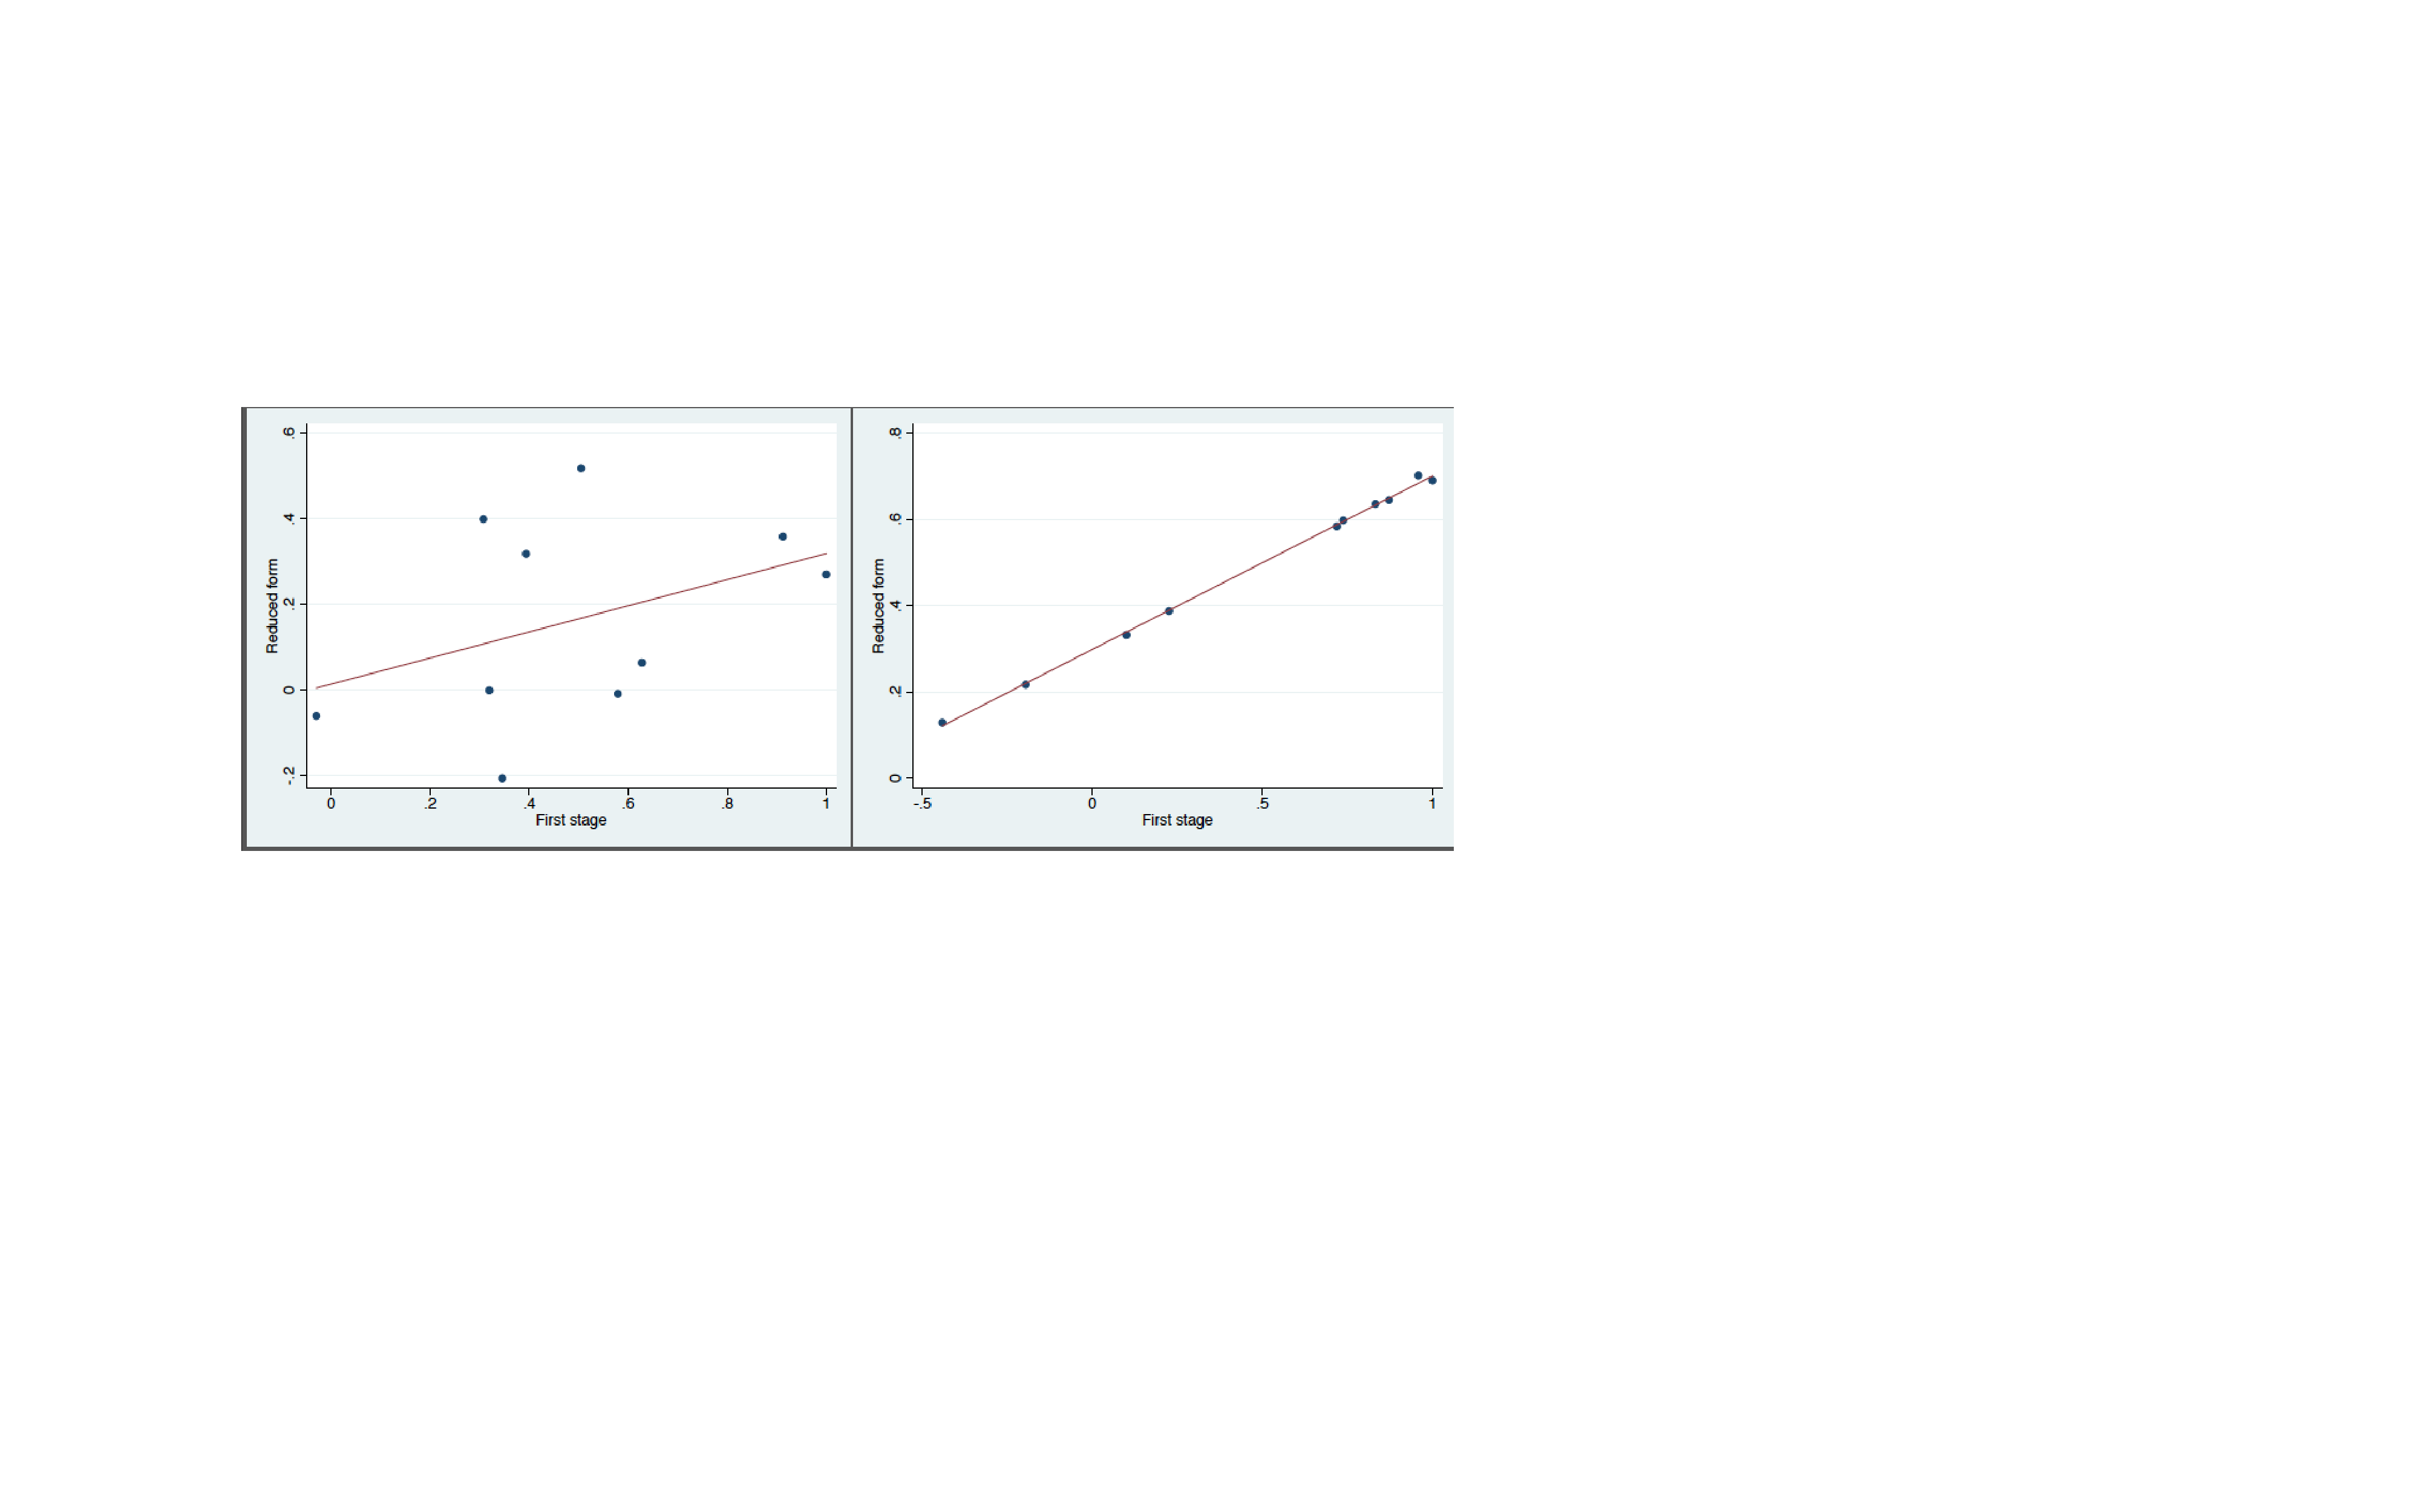
\includepdf{assets/6/overid_combined.pdf}

\begin{frame}{Testing Exclusion}

\begin{itemize}
\item {\footnotesize{}We can actually say something about exclusion even
with only one instrument and no covariates\medskip{}
}{\footnotesize\par}
\item {\footnotesize{}Suppose that the outcome, treatment, and instrument
are all binary \medskip{}
}{\footnotesize\par}
\item {\footnotesize{}We observe the treatment probabilities}{\footnotesize\par}
\end{itemize}
\begin{center}
{\footnotesize{}$ $$Pr\left[T_{i}=1|Z_{i}=1\right]=0.9$}{\footnotesize\par}
\par\end{center}

\begin{center}
{\footnotesize{}$Pr\left[T_{i}=1|Z_{i}=0\right]=0.8$}{\footnotesize\par}
\par\end{center}
\begin{itemize}
\item {\footnotesize{}We observe the outcome probabilities}{\footnotesize\par}
\end{itemize}
\begin{center}
{\footnotesize{}$Pr\left[Y_{i}=1|T_{i}=1,Z_{i}=1\right]=0.2$}{\footnotesize\par}
\par\end{center}

\begin{center}
{\footnotesize{}$Pr\left[Y_{i}=1|T_{i}=1,Z_{i}=0\right]=0.8$}{\footnotesize\par}
\par\end{center}

\begin{center}
{\footnotesize{}$Pr\left[Y_{i}=1|T_{i}=0,Z_{i}=1\right]=0.35$}{\footnotesize\par}
\par\end{center}

\begin{center}
{\footnotesize{}$Pr\left[Y_{i}=1|T_{i}=0,Z_{i}=0\right]=0.4$}{\footnotesize\par}
\par\end{center}
\begin{itemize}
\item {\footnotesize{}Notice anything?}{\footnotesize\par}
\end{itemize}
\end{frame}



\begin{frame}{Testing Exclusion }

\begin{itemize}
\item What is the share of always takers, $\pi_{at}$?
\medskip
\item What is the share of compliers, $\pi_{c}$?
\medskip
\item What is the share of never takers, $\pi_{nt}$?
\pause
\bigskip
\item Tell me how to identify $E[Y_{i}(1)\vert T_{i}(1)=1,T_{i}(0)=0]$.
\bigskip
\item Tell me what number you find for $E[Y_{i}(1)\vert T_{i}(1)=1,T_{i}(0)=0]$.
\bigskip
\item Tell me what you think is going on. 
\end{itemize}
\end{frame}

\begin{frame}{Testing Exclusion }

\begin{itemize}
\item {\small{}The first stage is too small to rationalize the difference
between the always taker mean outcome and the complier/always taker
mix\medskip{}
}{\small\par}
\item {\small{}There are not enough compliers to generate a drop from 0.8
to 0.2, even if all compliers have $Y_{i}(1)=0$\medskip{}
}{\small\par}
\item {\small{}This implies that $T_{i}$ cannot be the only channel through
which $Z_{i}$ affects $Y_{i}$}{\small\par}
\end{itemize}
\end{frame}

\begin{frame}{Testing Exclusion }

\begin{itemize}
\item {\footnotesize{}More generally, let $p^{at}=\pi^{at}/(\pi^{c}+\pi^{at})$
be the fraction of compliers in the $T_{i}=Z_{i}=1$ mixture. Then}{\footnotesize\par}
\end{itemize}
\begin{center}
{\footnotesize{}$E\left[Y_{i}(1)|T_{i}(1)=T_{i}(0)=1\right]\leq E\left[Y_{i}|Y_{i}\geq Q_{1-p^{at}}(Y_{i}|T_{i}=Z_{i}=1),T_{i}=Z_{i}=1\right]$}{\footnotesize\par}
\par\end{center}

\begin{center}
{\footnotesize{}$E\left[Y_{i}(1)|T_{i}(1)=T_{i}(0)=1\right]\geq E\left[Y_{i}|Y_{i}\leq Q_{p^{at}}(Y_{i}|T_{i}=Z_{i}=1),T_{i}=Z_{i}=1\right]$}{\footnotesize\par}
\par\end{center}
\begin{itemize}
\item {\footnotesize{}Under the most extreme possible assumptions, always
takers compose either the upper $p^{at}$ portion or the lower $p^{at}$
portion of the mixture distribution\medskip{}
}{\footnotesize\par}
\item {\footnotesize{}This generates bounds on the always taker means that
can be rationalized by the mixture}{\footnotesize\par}
\end{itemize}
\end{frame}

\begin{frame}{Testing Exclusion }

\begin{center}
{\footnotesize{}$E\left[Y_{i}(1)|T_{i}(1)=T_{i}(0)=1\right]\leq E\left[Y_{i}|Y_{i}\geq Q_{1-p^{at}}(Y_{i}|T_{i}=Z_{i}=1),T_{i}=Z_{i}=1\right]$}{\footnotesize\par}
\par\end{center}

\begin{center}
{\footnotesize{}$E\left[Y_{i}(1)|T_{i}(1)=T_{i}(0)=1\right]\geq E\left[Y_{i}|Y_{i}\leq Q_{p^{at}}(Y_{i}|T_{i}=Z_{i}=1),T_{i}=Z_{i}=1\right]$}{\footnotesize\par}
\par\end{center}
\begin{itemize}
\item {\footnotesize{}But the always taker mean is also point identified
as $E\left[Y_{i}|T_{i}=1,Z_{i}=0\right]$\medskip{}
}{\footnotesize\par}
\item {\footnotesize{}If the observed always taker mean is outside the bounds
implied by the mixture, the exclusion restriction must be violated}{\footnotesize\par}
\end{itemize}
\end{frame}

\begin{frame}{Testing Exclusion }

\begin{itemize}
\item {\footnotesize{}A similar argument can be used to bound the never
taker mean and compare the bounds to $E\left[Y_{i}|T_{i}=0,Z_{i}=1\right]$
\medskip{}
}{\footnotesize\par}
\item {\footnotesize{}Huber and Mellace (2015) propose a formal test of
the exclusion restriction based on this idea\medskip{}
}{\footnotesize\par}
\item {\footnotesize{}Kitagawa (2015) develops a related test that amounts
to checking whether complier CDFs are non-decreasing
\begin{itemize}
    \item {\footnotesize{}This paper provides a ``sharp'' result: the IV assumptions provide no other testable implications}
\end{itemize}
\medskip{}
}{\footnotesize\par}
\item {\footnotesize{}These tests are generalizations of the ``no first
stage sample'' idea: there is a limit on how large the reduced form
can be given the share of the population that complies\medskip{}
}{\footnotesize\par}
\item {\footnotesize{}Such tests may not be informative in practice since
the bounds will be wide unless the first stage is very small\medskip{}
}{\footnotesize\par}
\end{itemize}
\end{frame}



\begin{frame}{Continuous treatments}

Classic treatment is from Angrist and Imbens (1995)
\begin{itemize}
    \item Treatment is ordered for $j = 0, 1, .... J$
    \item Potential outcomes $Y(j)$
    \item Very natural for some things like prices, transfer amounts ... 
    \item Less natural for treatments like (no post secondary, trade school, university)
\end{itemize}

~\\
Single binary instrument $Z$
\begin{itemize}
    \item Monotonicity assumption: $Pr(D(1) \geq D(0)) = 1$ or $Pr(D(1) \leq D(0)) = 1$
    \item What does this mean? 
\end{itemize}
\end{frame}


\begin{frame}{Continuous treatments}
    Main result: Wald estimand is weighted average of \textbf{average causal responses} $Y(j) - Y(j-1)$

\begin{align*}
    \frac{ E[Y | Z{=}1] - E[Y | Z{=}0] }{E[D | Z{=}1] - E[D | Z{=}0]} = \sum_{j=1}^J \omega_j E[Y(j) - Y(j{-}1) \mid D(1) \geq j > D(0)]
\end{align*}

\begin{align*}
    \omega_j = \frac{P[D(1) \geq j > D(0)]}{\sum_{\ell=1}^J P[D(1) \geq \ell > D(0)] }
\end{align*}

Note that $\omega$ can be estimated!
\begin{itemize}
    \item Good practise to estimate/report the ACR weights
    \item Estimating complier means actually harder (see Garin et al 2024)
\end{itemize}

\end{frame}

\begin{frame}
\begin{center}
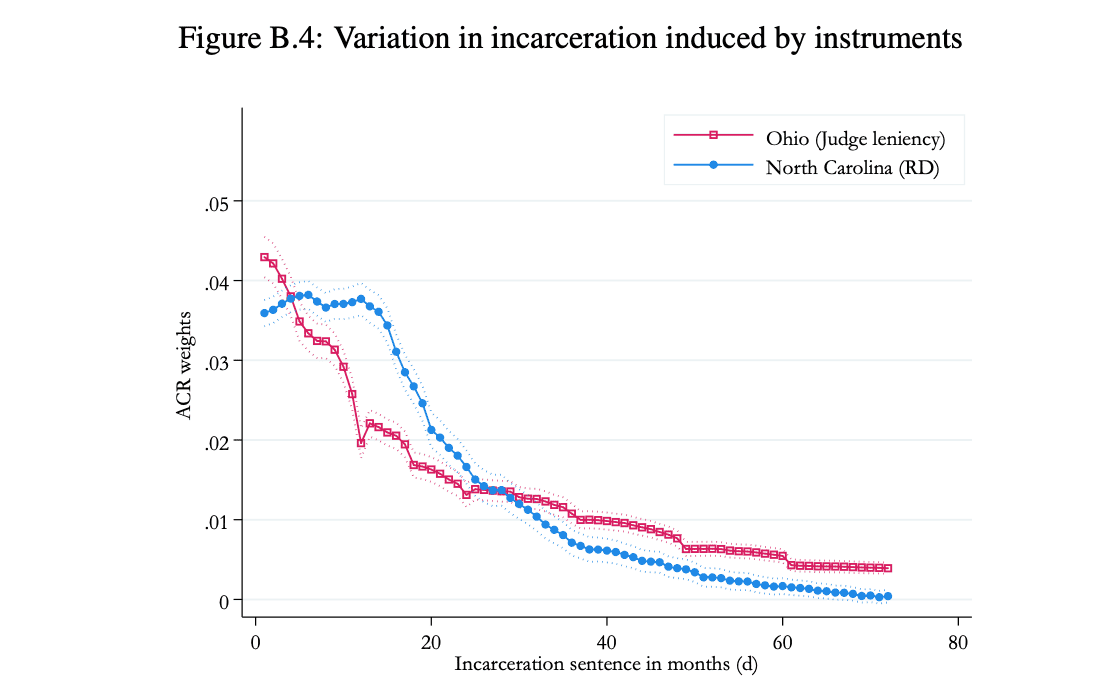
\includegraphics[scale=0.6]{assets/6/acr_wts.png}
\par\end{center}  
\end{frame}

\begin{frame}{Continuous treatments and exclusion}

Suppose that you have a continuous treatment like schooling $S$, and an instrument for it
\begin{itemize}
    \item Assume that it satisfies the Angrist and Imbens (1995) conditions
\end{itemize}

Define a new treatment, $T_i \equiv 1[S \geq 12]$. 
\begin{itemize}
    \item Can you instrument for that?
    \item Why or why not?
\end{itemize}

\pause
Requires assuming extensive margin compliers only (EMCO) (Rose and Shem-Tov, 2024) 
\begin{itemize}
    \item Some testable implications
    \item Remember: exclusion is instrument \textit{and} treatment specific!
\end{itemize}

    
\end{frame}


\begin{frame}{Final thoughts}

IV is a powerful tool to deal with omitted variable bias
\begin{itemize}
    \item Robust to heterogeneous effects
\end{itemize}

~\\
Often overlooked parts of thinking about an instrument:
\begin{itemize}
    \item Who does my instrument effect (compliers / relationship to ITT/TOT/TNT/ATE)
    \item What does my instrument do (ACR weights / exclusion / future mechanisms)
\end{itemize}
    
\end{frame}

\appendix
\begin{frame}
\centering
{\LARGE APPENDIX}\\[1em]
{\small Original many/weak slides, kept for comparison with the rewritten section. Also contains the trace derivation of the Bekker approximation.}
\end{frame}

\begin{frame}{IV in Finite Samples}

\begin{itemize}
\item {\small{}OLS is an unbiased
estimator of population projection coefficients in finite samples
(with a linear CEF or nonstochastic regressors)\medskip{}
}{\small\par}
\item {\small{}IV estimators do not have this property\medskip{}
}{\small\par}
\item {\small{}IV is a ratio of reduced form and first stage coefficients:}{\small\par}
\end{itemize}
\begin{center}
{\small{}$E\left[\hat{\rho}_{IV}\right]=E\left[\dfrac{\hat{\delta}}{\hat{\pi}}\right]$}{\small\par}
\par\end{center}

\begin{center}
{\small{}$\neq\dfrac{E\left[\hat{\delta}\right]}{E\left[\hat{\pi}\right]}$}{\small\par}
\par\end{center}

\begin{center}
{\small{}$=\rho$}{\small\par}
\par\end{center}

\end{frame}

\begin{frame}{IV in Finite Samples: Example}

\begin{itemize}
\item {\footnotesize{}Consider the following reduced form and first stage:}{\footnotesize\par}
\end{itemize}
\begin{center}
{\footnotesize{}$Y_{i}=\lambda+\delta Z_{i}+u_{i}$}{\footnotesize\par}
\par\end{center}

\begin{center}
{\footnotesize{}$S_{i}=\kappa+\pi Z_{i}+\eta_{i}$}{\footnotesize\par}
\par\end{center}
\begin{itemize}
\item {\footnotesize{}Suppose the instruments are non-stochastic, and }{\footnotesize\par}
\end{itemize}
\begin{center}
{\footnotesize{}$(u_{i},\eta_{i})\sim N\left(0,\left[\begin{array}{cc}
\sigma_{u}^{2} & \tau\sigma_{u}\sigma_{\eta}\\
\tau\sigma_{u}\sigma_{\eta} & \sigma_{\eta}^{2}
\end{array}\right]\right)$}{\footnotesize\par}
\par\end{center}
\begin{itemize}
\item {\footnotesize{}Then the finite-sample distribution of the reduced
form and first stage coefficients is}{\footnotesize\par}
\end{itemize}
\begin{center}
{\footnotesize{}$\left(\hat{\delta},\hat{\pi}\right)\sim N\left((\delta,\pi),\left[\begin{array}{cc}
\sigma_{u}^{2}\left[\sum_{i}(Z_{i}-\bar{Z})^{2}\right]^{-1} & \tau\sigma_{u}\sigma_{\eta}\left[\sum_{i}(Z_{i}-\bar{Z})^{2}\right]^{-1}\\
\tau\sigma_{u}\sigma_{\eta}\left[\sum_{i}(Z_{i}-\bar{Z})^{2}\right]^{-1} & \sigma_{\eta}^{2}\left[\sum_{i}(Z_{i}-\bar{Z})^{2}\right]^{-1}
\end{array}\right]\right)$}{\footnotesize\par}
\par\end{center}

\end{frame}

\begin{frame}{IV in Finite Samples: Example}

\begin{itemize}
\item The IV coefficient, $\hat{\rho}=\hat{\delta}/\hat{\pi}$, is a ratio
of two jointly normal random variables{\small{}\medskip{}
}{\small\par}
\item $\hat{\rho}$ therefore follows a normal ratio distribution {\small{}\medskip{}
}{\small\par}
\item Normal ratio distributions do not have moments, so $E\left[\hat{\rho}\right]$,
$Var\left(\hat{\rho}\right)$, and all higher moments do not exist.
In this sense $\hat{\rho}$ is biased{\small{}\medskip{}
}{\small\par}
\item If $\tau=0$ and $\pi\rightarrow0$, $\hat{\rho}$ becomes the ratio
of two independent mean zero normals, which follows a Cauchy distribution
(see Nelson and Starz 1990 for more)
\end{itemize}
\end{frame}

\begin{frame}{IV in Finite Samples: Many/Weak Problems}

\begin{itemize}
\item {\footnotesize{}In general, just-identified IV estimators have no
moments and fat tails\medskip{}
}{\footnotesize\par}
\item {\footnotesize{}However, just-id estimators are approximately centered
in the right place in the sense that $Q_{0.5}(\hat{\rho}_{IV})\approx\rho$
(more details later)\medskip{}
}{\footnotesize\par}
\item {\footnotesize{}It turns out that overidentified IV estimators are
not centered at the right place: they are biased towards OLS\medskip{}
}{\footnotesize\par}
\item {\footnotesize{}The severity of finite-sample bias increases with
the degree of overfitting AND as the first-stage relationship
between instruments and endogenous regressors gets weaker\medskip{}
}{\footnotesize\par}
\item {\footnotesize{}IV bias is therefore worse when the instruments are
``many/weak''\medskip{}
}{\footnotesize\par}
\item {\footnotesize{}Bound, Jaeger and Baker (1995) showed that this problem
can be important in practice, spawning a large literature on dealing
with many/weak instruments}{\footnotesize\par}
\end{itemize}
\end{frame}

\begin{frame}{Bound, Jaeger and Baker (1995)}

\begin{itemize}
\item {\footnotesize{}Bound, Jaeger and Baker (1995) revisit the Angrist/Krueger
QOB instrument\medskip{}
}{\footnotesize\par}
\item {\footnotesize{}The Wald estimates we studied are just-identified,
so the many/weak critique does not apply (a common misconception)
\medskip{}
}{\footnotesize\par}
\item {\footnotesize{}However, AK also estimate overidentified 2SLS models
of the form}{\footnotesize\par}
\end{itemize}
\begin{center}
{\footnotesize{}$Y_{i}=\rho S_{i}+\sum_{b=1}^{50}\theta_{b}B_{ib}+\sum_{t=1}^{30}\psi_{t}T_{it}+\varepsilon_{i}$}{\footnotesize\par}
\par\end{center}

\begin{center}
{\footnotesize{}$S_{i}=\sum_{q=1}^{3}\left[\sum_{b=1}^{50}\pi_{qb}B_{ib}Q_{iq}+\sum_{t=1}^{30}\tau_{qt}T_{it}Q_{iq}\right]$}{\footnotesize\par}
\par\end{center}

\begin{center}
{\footnotesize{}$+\sum_{b=1}^{50}\kappa_{b}B_{ib}+\sum_{t=1}^{30}\phi_{t}T_{it}+\eta_{i}$}{\footnotesize\par}
\par\end{center}
\begin{itemize}
\item {\footnotesize{}Here $B_{ib}$ is a dummy for birth in state $b$,
$T_{it}$ is a dummy for birth in year $t$, and $Q_{iq}$ is a dummy
for birth in quarter $q$}{\footnotesize\par}
\end{itemize}
\end{frame}

\begin{frame}{Bound, Jaeger and Baker (1995)}

\begin{itemize}
\item {\footnotesize{}The AK model uses 30 quarter/year and 150 quarter/state
interactions as instruments, so is overidentified by 179\medskip{}
}{\footnotesize\par}
\item {\footnotesize{}The interactions are meant to capture differences
in the effects of compulsory schooling laws across states and over
time\medskip{}
}{\footnotesize\par}
\item {\footnotesize{}From the point of view of 2SLS asymptotics, adding
the interactions can only be a plus: more instruments improve the
first stage fit and drive down standard errors\medskip{}
}{\footnotesize\par}
\item {\footnotesize{}But the QOB first stage is small and many of the interactions
are likely to be irrelevant, so this is a severe many/weak scenario\medskip{}
}{\footnotesize\par}
\item {\footnotesize{}Bound, Jaeger and Baker replace the QOB dummies with
randomly-generated fake QOB variables that have no first stage by
design}{\footnotesize\par}
\end{itemize}
\end{frame}

\begin{frame}{Bound, Jaeger and Baker (1995)}

\begin{center}
{\footnotesize{}}%
\begin{tabular}{|c|c|c|c|}
\hline 
 & {\footnotesize{}2SLS (real QOB)} & {\footnotesize{}2SLS (fake QOB)} & {\footnotesize{}OLS}\tabularnewline
\hline 
\hline 
{\footnotesize{}30 QOB{*}year} & {\footnotesize{}0.081} & {\footnotesize{}0.062} & {\footnotesize{}0.063}\tabularnewline
\hline 
{\footnotesize{}interactions} & {\footnotesize{}(0.016)} & {\footnotesize{}(0.037)} & {\footnotesize{}(0.000)}\tabularnewline
\hline 
 &  &  & \tabularnewline
\hline 
{\footnotesize{}180 QOB{*}year and state} & {\footnotesize{}0.083} & {\footnotesize{}0.060} & {\footnotesize{}0.063}\tabularnewline
\hline 
{\footnotesize{}interactions} & {\footnotesize{}(0.009)} & {\footnotesize{}(0.015)} & {\footnotesize{}(0.000)}\tabularnewline
\hline 
\end{tabular}{\footnotesize\par}
\par\end{center}

\end{frame}

\begin{frame}{Bound, Jaeger and Baker (1995)}

\begin{itemize}
\item {\small{}The Bound, Jaeger and Baker results show that the AK 2SLS
specification essentially reproduces OLS even if the instruments are
junk unrelated to schooling\medskip{}
}{\small\par}
\item {\small{}Disturbingly, conventional IV standard errors give no indication
of the extent of the problem\medskip{}
}{\small\par}
\item {\small{}The fake QOB 180-instrument model generates an estimate that
looks precise despite the lack of a first stage\medskip{}
}{\small\par}
\item {\small{}How can we diagnose many/weak problems, and correct them
if they are present?}{\small\par}
\end{itemize}
\end{frame}

\begin{frame}{Many/Weak Bias}

\begin{itemize}
\item {\small{}Consider a model with a single endogenous regressor and $Q$
instruments, written in matrix form:}{\small\par}
\end{itemize}
\begin{center}
$Y=\rho S+\varepsilon$
\par\end{center}

\begin{center}
$S=Z\pi+\eta$
\par\end{center}
\begin{itemize}
\item Remember that we can write $\hat{S}=P_{Z}S$
\item We can thus re-write the 2SLS estimator of $\rho$ (regression of $Y$ on $\hat{S}$) as 
\end{itemize}
\begin{center}
$\hat{\rho}_{2SLS}=\rho+(S^{\prime}P_{Z}S)^{-1}S^{\prime}P_{Z}\varepsilon$
\par\end{center}

\begin{center}
$=\rho+\left(S^{\prime}P_{Z}S\right)^{-1}(\pi^{\prime}Z^{\prime}+\eta^{\prime})P_{Z}\varepsilon$
\par\end{center}

\begin{center}
$=\rho+(S^{\prime}P_{Z}S)^{-1}\pi^{\prime}Z^{\prime}\varepsilon+\left(S^{\prime}P_{Z}S\right)^{-1}\eta^{\prime}P_{Z}\varepsilon$
\par\end{center}

\end{frame}

\begin{frame}{Many/Weak Bias}

\begin{center}
{\small{}$E\left[\hat{\rho}_{2SLS}-\rho\right]=E\left[(S^{\prime}P_{Z}S)^{-1}\pi^{\prime}Z^{\prime}\varepsilon\right]+E\left[\left(S^{\prime}P_{Z}S\right)^{-1}\eta^{\prime}P_{Z}\varepsilon\right]$}{\small\par}
\par\end{center}
\begin{itemize}
\item {\small{}It's difficult to make further progress since we cannot pass
expectations inside the inverse\medskip{}
}{\small\par}
\item {\small{}Bekker (1994): passing the expectations through provides
an accurate approximation under group asymptotics that allow $Q$
to grow with $N$\medskip{}
}{\small\par}
\item {\small{}Then the finite-sample bias of 2SLS can be approximated}{\small\par}
\end{itemize}
\begin{center}
{\small{}$E\left[\hat{\rho}_{2SLS}-\rho\right]\approx(E\left[S^{\prime}P_{Z}S\right])^{-1}\pi^{\prime}E\left[Z^{\prime}\varepsilon\right]+\left(E\left[S^{\prime}P_{Z}S\right]\right)^{-1}E\left[\eta^{\prime}P_{Z}\varepsilon\right]$}{\small\par}
\par\end{center}

\end{frame}

\begin{frame}{Many/Weak Bias}

\begin{center}
{\small{}$E\left[\hat{\rho}_{2SLS}-\rho\right]\approx(E\left[S^{\prime}P_{Z}S\right])^{-1}\pi^{\prime}E\left[Z^{\prime}\varepsilon\right]+\left(E\left[S^{\prime}P_{Z}S\right]\right)^{-1}E\left[\eta^{\prime}P_{Z}\varepsilon\right]$}{\small\par}
\par\end{center}
\begin{itemize}
\item {\small{}The first term is zero (why)?\medskip{}
}{\small\par}
\item {\small{}The finite-sample bias of 2SLS comes from the fact that the
numerator of the second term is not zero:\medskip{}
}{\small\par}
\end{itemize}
\begin{center}
$E\left[\eta^{\prime}P_{Z}\varepsilon\right]\neq0$
\par\end{center}
\begin{itemize}
\item What is the intuition for this?
\end{itemize}
\end{frame}


\begin{frame}{Many/Weak Bias}

\begin{itemize}
\item {\footnotesize{}To make further progress, let's use some matrix tricks}

\begin{itemize}
\item {\footnotesize{}A scalar equals its trace}{\footnotesize\par}
\item {\footnotesize{}Trace is invariant to cyclic permutations}{\footnotesize\par}
\item {\footnotesize{}Trace is a linear operator that passes through expectations}{\footnotesize\par}
\end{itemize}
\end{itemize}
\begin{center}
{\footnotesize{}$E\left[\eta^{\prime}P_{Z}\varepsilon|Z\right]=E\left[tr\left(\eta^{\prime}P_{Z}\varepsilon\right)|Z\right]$}{\footnotesize\par}
\par\end{center}

\begin{center}
{\footnotesize{}$=E\left[tr\left(P_{Z}\varepsilon\eta^{\prime}\right)|Z\right]$}{\footnotesize\par}
\par\end{center}

\begin{center}
{\footnotesize{}$=tr\left(P_{Z}E\left[\varepsilon\eta^{\prime}|Z\right]\right)$}{\footnotesize\par}
\par\end{center}

\begin{center}
{\footnotesize{}$=\sigma_{\eta\varepsilon}tr\left(Z(Z^{\prime}Z)^{-1}Z^{\prime}\right)$}{\footnotesize\par}
\par\end{center}

\begin{center}
{\footnotesize{}$=\sigma_{\eta\varepsilon}tr\left((Z^{\prime}Z)^{-1}Z^{\prime}Z\right)$}{\footnotesize\par}
\par\end{center}

\begin{center}
{\footnotesize{}$=\sigma_{\eta\varepsilon}Q$}{\footnotesize\par}
\par\end{center}

\end{frame}

\begin{frame}{Many/Weak Bias}

\begin{itemize}
\item {\footnotesize{}The denominator of the bias is}{\footnotesize\par}
\end{itemize}
\begin{center}
{\footnotesize{}$E\left[S^{\prime}P_{Z}S\right]=E\left[(\pi^{\prime}Z^{\prime}+\eta^{\prime})P_{Z}(Z\pi+\eta)\right]$}{\footnotesize\par}
\par\end{center}

\begin{center}
{\footnotesize{}$=E\left[\pi^{\prime}Z^{\prime}Z\pi\right]+E\left[\eta^{\prime}P_{Z}\eta\right]$}{\footnotesize\par}
\par\end{center}
\begin{itemize}
\item {\footnotesize{}Applying the same trace tricks to the second term
shows that $E\left[\eta^{\prime}P_{Z}\eta\right]=\sigma_{\eta}^{2}Q$}{\small{}\medskip{}
}{\small\par}
\item {\footnotesize{}Then}{\footnotesize\par}
\end{itemize}
\begin{center}
{\footnotesize{}$E\left[\hat{\rho}_{2SLS}-\rho\right]\approx\dfrac{\sigma_{\eta\varepsilon}Q}{E\left[\pi^{\prime}Z^{\prime}Z\pi\right]+\sigma_{\eta}^{2}Q}$}{\footnotesize\par}
\par\end{center}

\begin{center}
{\footnotesize{}$=\dfrac{\sigma_{\eta\varepsilon}}{\sigma_{\eta^{2}}}\cdot\dfrac{1}{1+E\left[\pi^{\prime}Z^{\prime}Z\pi\right]/(\sigma_{\eta}^{2}Q)}$}{\footnotesize\par}
\par\end{center}

\end{frame}

\begin{frame}{Many/Weak Bias}

\begin{center}
{\small{}$E\left[\hat{\rho}_{2SLS}-\rho\right]\approx\dfrac{\sigma_{\eta\varepsilon}}{\sigma_{\eta^{2}}}\cdot\dfrac{1}{1+E\left[\pi^{\prime}Z^{\prime}Z\pi\right]/(\sigma_{\eta}^{2}Q)}$}{\small\par}
\par\end{center}
\begin{itemize}
\item {\small{}Notice that $E\left[\pi^{\prime}Z^{\prime}Z\pi\right]$ is
the explained sum of squares from the regression of $S$ on $Z$,
while $\sigma_{\eta}^{2}$ is the residual sum of squares divided
by $N$\medskip{}
}{\small\par}
\item {\small{}Then }{\small\par}
\end{itemize}
\begin{center}
{\small{}$E\left[\hat{\rho}_{2SLS}-\rho\right]\approx\dfrac{\sigma_{\eta\varepsilon}}{\sigma_{\eta^{2}}}\cdot\dfrac{1}{1+F}$}{\small\par}
\par\end{center}
\begin{itemize}
\item {\small{}Here $F$ is the first stage (population) $F$-statistic for the joint
significance of all the instruments}{\small\par}
\end{itemize}
\end{frame}

\begin{frame}{Many/Weak Bias}

\begin{center}
{\small{}$E\left[\hat{\rho}_{2SLS}-\rho\right]=\dfrac{\sigma_{\eta\varepsilon}}{\sigma_{\eta^{2}}}\cdot\dfrac{1}{1+F}$}{\small\par}
\par\end{center}
\begin{itemize}
\item {\small{}Note also that when $F$ goes to zero, the 2SLS bias becomes
$\sigma_{\eta\varepsilon}/\sigma_{\eta}^{2}$\medskip{}
}{\small\par}
\item {\small{}With a zero first stage, $S=\eta$ so $\sigma_{\eta\varepsilon}/\sigma_{\eta}^{2}=Cov(S_{i},\varepsilon_{i})/Var(S_{i})$,
the bias of OLS\medskip{}
}{\small\par}
\item {\small{}As the first stage shrinks to zero, all of the variance in
the fitted values comes from the endogenous part of $\hat{S}$, and
the bias of 2SLS equals the bias of OLS}{\small\par}
\end{itemize}
\end{frame}

\begin{frame}{Many/Weak In Practice}

\begin{itemize}
\item {\small{}In practice it is a good idea to look at the first stage
$F$-statistic \medskip{}
}{\small\par}
\item {\small{}In models with exogenous controls this should be the }\emph{\small{}partial
$F$ }{\small{}on the excluded instruments\medskip{}
}{\small\par}
\item {\small{}Stock and Staiger (1997) suggest that many weak typically
becomes a problem when $F<10$, though this is not a theorem\medskip{}
}{\small\par}
\item {\small{}Standard errors based on Bekker (1994) asymptotics are more
accurate in many/weak scenarios (see also Hansen et al. 2008)}{\small\par}
\end{itemize}
\end{frame}

\begin{frame}{Many/Weak In Practice}

\begin{itemize}
\item {\footnotesize{}The Limited Information Maximum Likelihood (LIML)
estimator coincides with 2SLS for just-id models and is approximately
median unbiased for overidentified models \medskip{}
}{\footnotesize\par}
\item {\footnotesize{}A comparison of LIML and 2SLS can help determine whether
many/weak is a problem (though conventional LIML standard errors are
too small) \medskip{}
}{\footnotesize\par}
\item {\footnotesize{}LIML has some unattractive features, however: it has
fat tails (no moments), and is inconsistent with heteroskedasticity\medskip{}
}{\footnotesize\par}
\item {\footnotesize{}There are other estimators (e.g. Fuller) that correct
some of the deficiencies of LIML; see Stock and Yogo (2005)\medskip{}
}{\footnotesize\par}
\item {\footnotesize{}The Anderson-Rubin (AR) test provides a method for
testing hypotheses about $\rho$ that is robust to weak instruments,
though it has low power when the instruments are weak}{\footnotesize\par}
\end{itemize}
\end{frame}
%%
\begin{frame}{The Judges Design}

\begin{itemize}
\item {\footnotesize{}But when it sensible to talk about a research design with ``many" instruments?
$\rightarrow$ a research design that uses differences
in the harshness/leniency of judges or other examiners is a research design that often has to deal with many/weak potential problems\medskip{}
}{\footnotesize\par}
\item {\footnotesize{}Examples: Kling (2006) on criminal sentencing, Doyle
(2007) on foster care, Maestas et al. (2013) on disability insurance,
Dobbie (2015) on bankruptcy \medskip{}
}{\footnotesize\par}
\item {\footnotesize{}If judges are randomly assigned, the identity of the
judge is a plausible instrument (there are many fixed effects for judges!)\medskip{}
}{\footnotesize\par}
\end{itemize}
\end{frame}

\begin{frame}{The Judges Design}

\begin{itemize}
\item {\small{}Common approach to the judges design: Define}{\small\par}
\end{itemize}
\begin{center}
{\small{}$T_{i}^{*}=\dfrac{1}{n_{j(i)}-1}{\displaystyle \sum_{k\neq i}1\left\{ j(k)=j(i)\right\} T_{k}}$}{\small\par}
\par\end{center}
\begin{itemize}
\item {\small{}$T_{i}^{*}$ is the mean treatment rate (e.g. incarceration
rate) for the judge assigned to $i$, $j(i)$, for all cases not involving
$i$\medskip{}
}{\small\par}
\item {\small{}$T_{i}^{*}$ is then used as an instrument for $i$'s actual
treatment $T_{i}$}{\small\par}
\end{itemize}
\end{frame}

\begin{frame}{The Judges Design: JIVE}

\begin{itemize}
\item {\small{}Note that $T_{i}^{*}$ is the fitted value from a first stage
regression of removal on all the judge dummies, leaving out $i$\medskip{}
}{\small\par}
\item {\small{}The instruments are implicitly a full set of judge dummies,
which may lead to many/weak problems\medskip{}
}{\small\par}
\item {\small{}Using a leave-out mean changes the estimator from 2SLS to
jackknife IV (JIVE), which is one solution to the many/weak problem
but not necessarily the optimal one\medskip{}
}{\small\par}
\item {\small{}Conventional standard errors for JIVE are also incorrect
in many/weak scenarios.}{\small\par}
\medskip
\item {\small{}Despite this, many papers use judges design given its implicit attractiveness plus the possibility to summarize nicely heterogenous treatment effects (see the marginal treatment effects literature pioneered by Heckman and Vytacil, 1999,2005).  }{\small\par}
\end{itemize}
\end{frame}

\end{document}
